\documentclass[aspectratio=169]{beamer}
\usepackage{lmodern}
\usetheme{Madrid}
%\usecolortheme{giantoak}
\newcommand*\oldmacro{}
\let\oldmacro\insertshorttitle
\renewcommand*\insertshorttitle{\oldmacro\hfill\insertframenumber\,/\,\inserttotalframenumber}
\usepackage[framemethod=tikz]{mdframed}

\usepackage{beamerthemesplit}
\usepackage{textpos}
\usepackage{pgf}
%\logo{\pgfputat{\pgfxy(0,-.4)}{\pgfbox[right,base]{\includegraphics[height=1.0cm]{logo.jpg}}}}
%\newcommand{\nologo}{\setbeamertemplate{logo}{}}
\usepackage{booktabs}
\usepackage{graphicx}
\theoremstyle{principle}
\newtheorem*{principle}{Design Principle}


\titlegraphic{\includegraphics[width=1.0\paperwidth]{cool-wind-800px.jpg}}

\title{Amendments}
%\author[Jeremy Kedziora]{Wind Data Science Team\\
%\small{Uptake}}
\date{}

\begin{document}

%{
%%\nologo
%\begin{frame}
%    \maketitle
%\end{frame}
%}
%pages 1-7, 8-9, 14-15.


{
  \usebackgroundtemplate{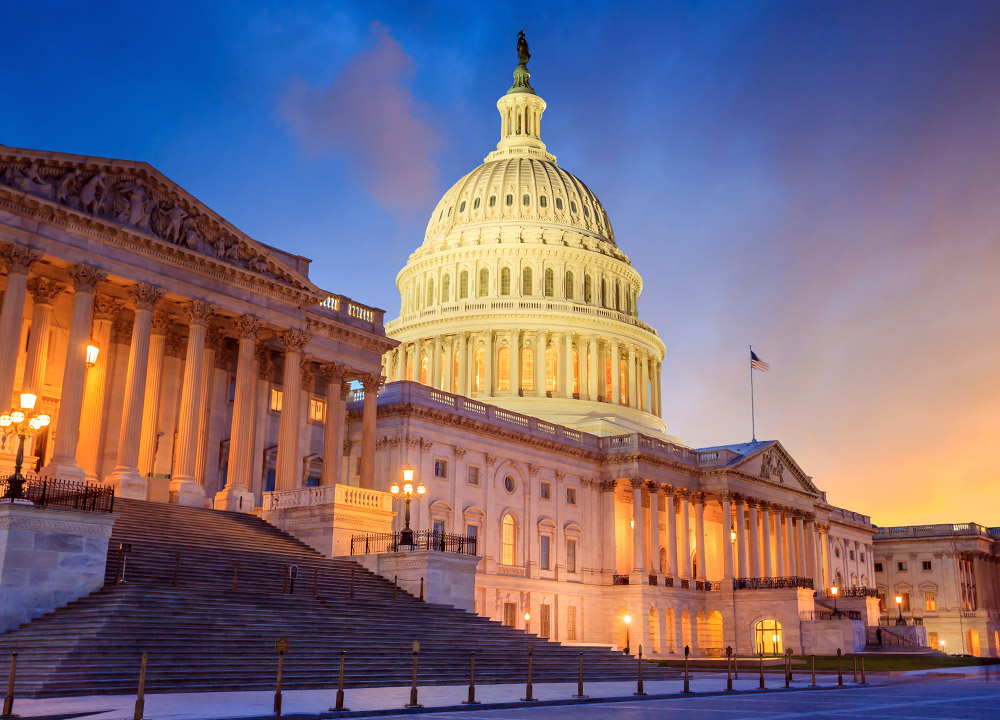
\includegraphics[width=1.0\paperwidth]{capitol.jpg}}
  \begin{frame}[plain]
  
\begin{mdframed}[tikzsetting={draw=black,fill=white,fill opacity=0.7,
               line width=0pt},backgroundcolor=none,leftmargin=20,
               rightmargin=20,innertopmargin=4pt]
\Huge Birkland
\end{mdframed}

  \end{frame}
}

%@@@@@@@@@@@@@@@@@@@@@@@@@@@@@@@@@@@@@@@@@@@@@@@@@
%\begin{frame}
%
%\begin{center}
%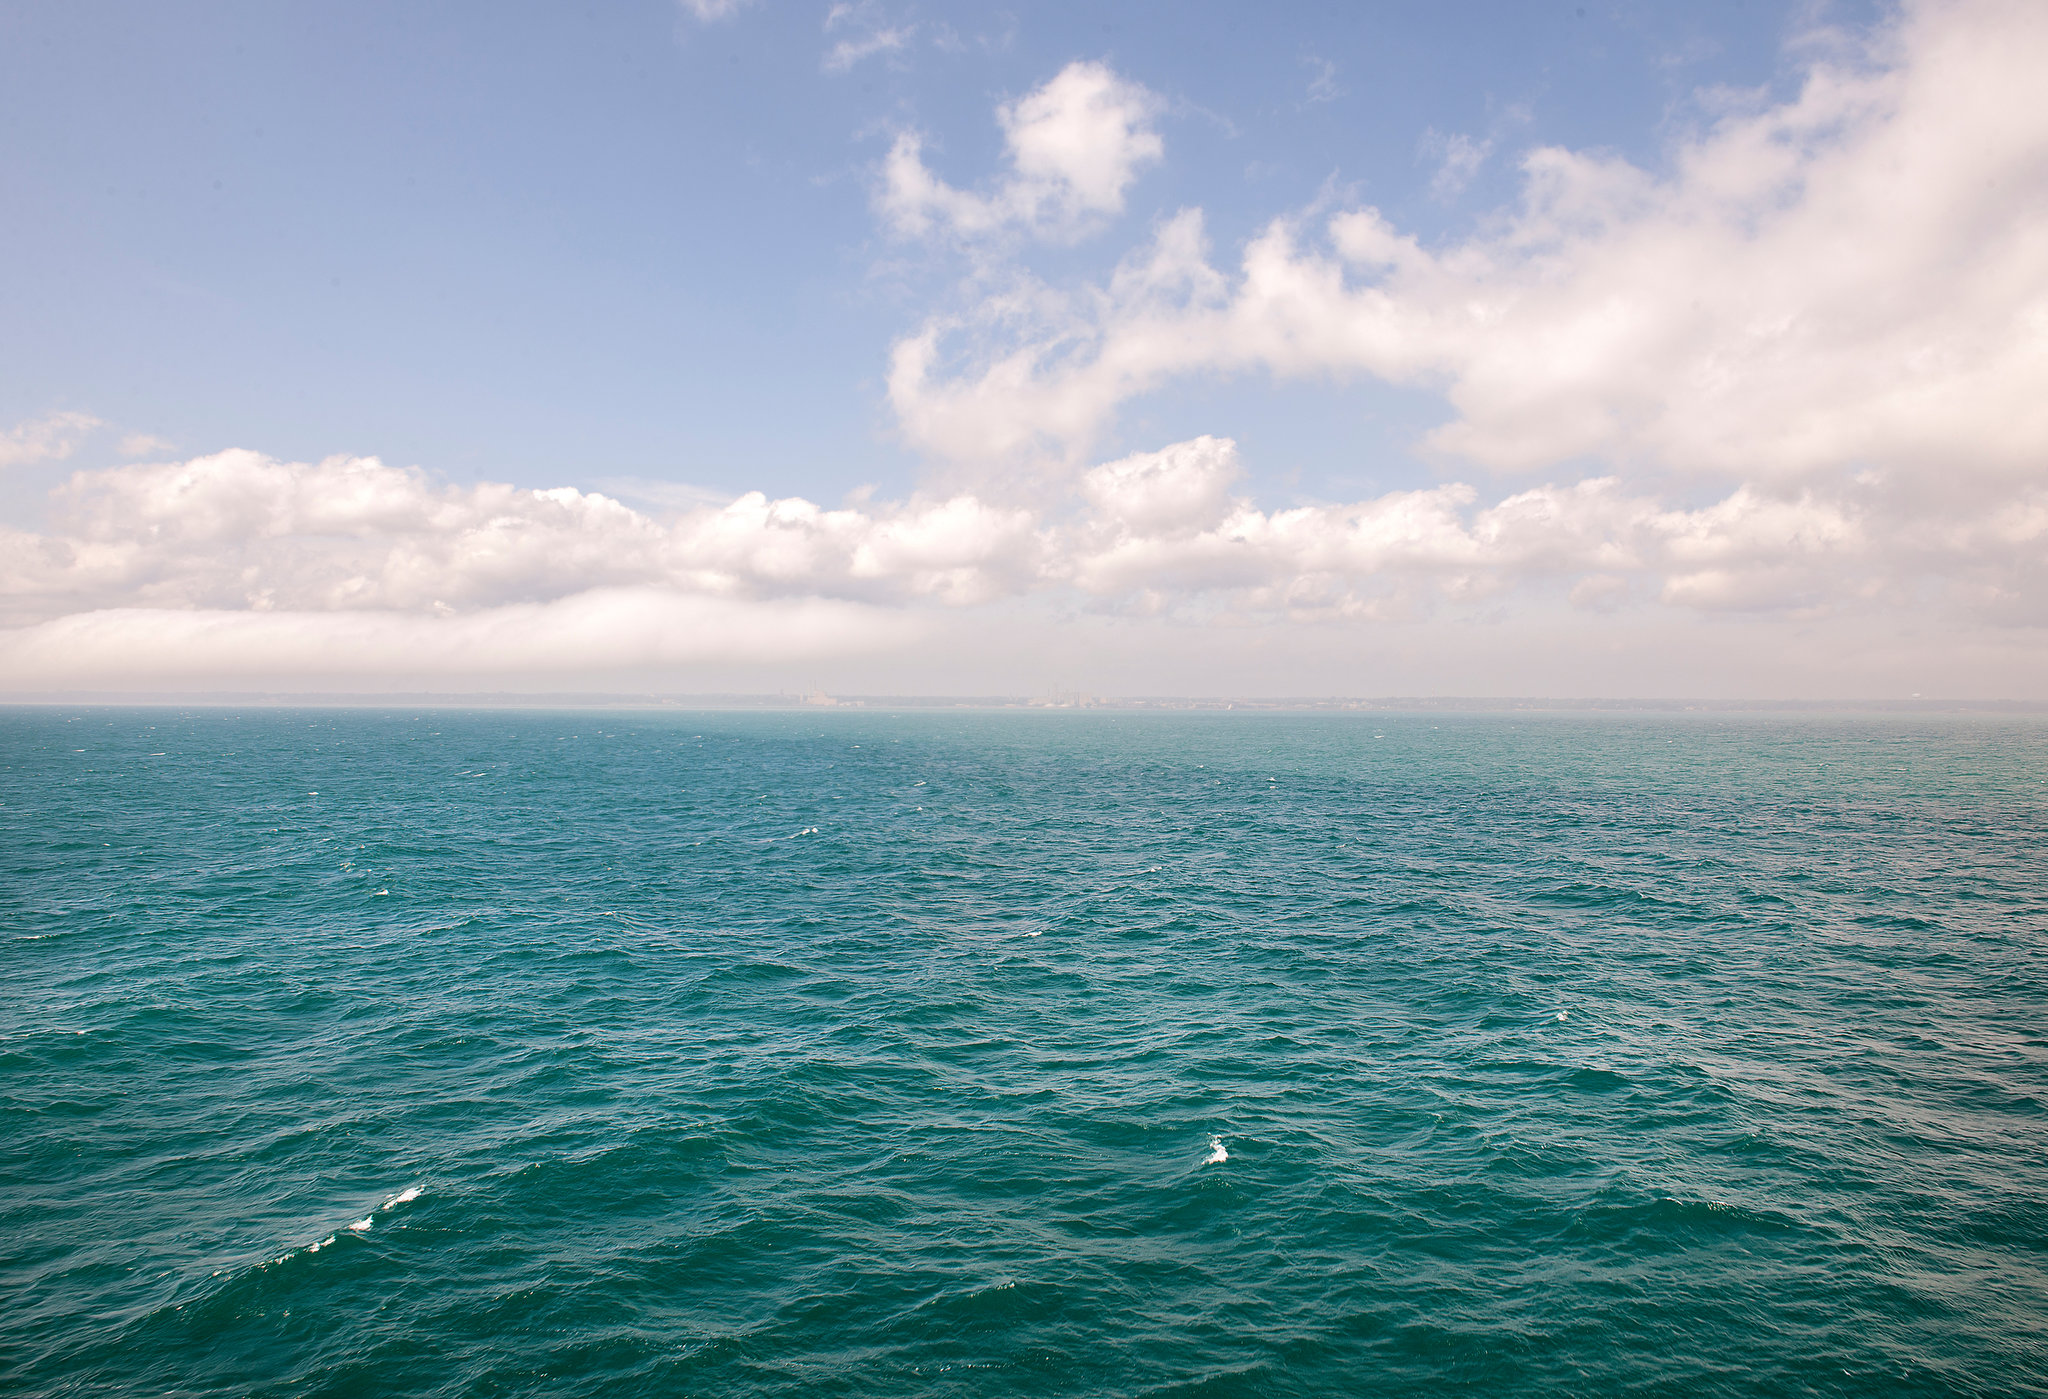
\includegraphics[scale=0.4]{lake_michigan.jpg}
%\end{center}
%
%
%\end{frame}

\begin{frame}
\begin{center}
\Huge\textbf{What is politics?}
\end{center}
\end{frame}

%@@@@@@@@@@@@@@@@@@@@@@@@@@@@@@@@@@@@@@@@@@@@@@@@@
\begin{frame}
\frametitle{What is politics?}
\begin{itemize}
\item the art or science of government;
\bigskip
\bigskip
\item collective action;
\bigskip
\bigskip
\item participation in civic life;
\end{itemize}

\end{frame}

%@@@@@@@@@@@@@@@@@@@@@@@@@@@@@@@@@@@@@@@@@@@@@@@@@
\begin{frame}
\frametitle{What is politics?}
\begin{center}
\Huge\textbf{The authoritative distribution of resources.}
\end{center}
\end{frame}

%@@@@@@@@@@@@@@@@@@@@@@@@@@@@@@@@@@@@@@@@@@@@@@@@@
\begin{frame}
\begin{center}
\Huge\textbf{What is policy?}
\end{center}
\end{frame}

%@@@@@@@@@@@@@@@@@@@@@@@@@@@@@@@@@@@@@@@@@@@@@@@@@
\begin{frame}
\frametitle{What is policy?}

\begin{itemize}
\item the actions of government and the intentions that determine those actions (Cochran et al 2010);
\bigskip
\item the outcome of the struggle in government of who gets what (Cochran et al 2010);
\bigskip
\item whatever governments choose to do or not to do (Dye 2013);
\bigskip
\item political decisions for implementing programs to achieve societal goals (Cochran and Malone 2010);
\bigskip
\item the sum of government activity, whether acting directly or through agents (Peters 2010);
\end{itemize}
\end{frame}

%@@@@@@@@@@@@@@@@@@@@@@@@@@@@@@@@@@@@@@@@@@@@@@@@@
\begin{frame}
\frametitle{What is policy?}
\begin{center}
\begin{itemize}
\item \huge\textbf{Statement by government of what it intends to do to solve a problem... (Birkland)}
\bigskip
\item \huge\textbf{... commitment to solve the problem in a similar way in the future. (me)}
\end{itemize}
\end{center}
\end{frame}

%%@@@@@@@@@@@@@@@@@@@@@@@@@@@@@@@@@@@@@@@@@@@@@@@@@
%\begin{frame}
%\frametitle{Public Policy}
%
%Policy is:
%\begin{itemize}
%\item a response to a \textbf{problem}...
%\bigskip
%\item ...made on the \textbf{public's} behalf...
%\bigskip
%\item ...oriented toward \textbf{solving} the problem...
%\bigskip
%\item ...formulated by \textbf{government}...
%\bigskip
%\item \textbf{interpreted} by the public.
%\end{itemize}
%\end{frame}

%@@@@@@@@@@@@@@@@@@@@@@@@@@@@@@@@@@@@@@@@@@@@@@@@@
\begin{frame}
\frametitle{What is policy?}

\begin{itemize}
\item \textbf{Explicit policy} -- articulated policy statement:
\begin{itemize}
\item Constitution;
\item Statute law, budget;
\item Executive order, regulatory rule;
\item Court precedent;
\end{itemize}
\bigskip
\bigskip
\item \textbf{Implicit policy} -- lack of a definitive policy statement:
\begin{itemize}
\item Constitutional guarantees of healthcare, housing, living wage, etc.
\item Front line bureaucrats, e.g. teachers, election officials, police officers..
\end{itemize}

\end{itemize}
\end{frame}

%@@@@@@@@@@@@@@@@@@@@@@@@@@@@@@@@@@@@@@@@@@@@@@@@@
\begin{frame}
\frametitle{Branches of Study}

\begin{itemize}
\item \textbf{Public Policy Research}: application of social science in support of public policy decision evaluation for specific problems;
\bigskip
\bigskip

\item \textbf{Comparative Public Policy}: how do different entities formulate solutions to problems? Descriptive, cross-national, or cross-state;
\bigskip
\bigskip

\item \textbf{Public Policy Processes}: academic research on how political actors formulate and implement public policy (much of the rest of the class);
\bigskip
\bigskip

\item \textbf{Public Policy Analysis}: application of logic and mix of techniques in support of public policy decision making.  Borrows heavily from economics. Focus on problem specification, generation of alternative policies, and assessment of policies in support of public policy decision making.  Evidence. (practice via memos);

\end{itemize}
\end{frame}

%%@@@@@@@@@@@@@@@@@@@@@@@@@@@@@@@@@@@@@@@@@@@@@@@@@
%\begin{frame}
%\frametitle{Definitions}
%
%\begin{itemize}
%\item \textbf{Problem}: A usually undesirable situation that, according to people or interest groups, can be alleviated by government action.
%\begin{itemize}
%\item A policy is \textbf{Pareto Optimal} is nobody can be made better off without somebody being made worse off;
%\end{itemize}
%\bigskip
%\bigskip
%\item \textbf{Public interest}: The assumed broader desires and needs of the public, in whose name policy is made.
%\bigskip
%\bigskip
%\bigskip
%\item \textbf{Classical liberalism}: ideological system that emphasizes individual liberty and the ownership and acquisition of private property as a means to improve overall wealth and happiness and discourage social strife (e.g. Locke's Second Treatise of Civil Government 1690, very influential for framers).
%\end{itemize}
%\end{frame}

%@@@@@@@@@@@@@@@@@@@@@@@@@@@@@@@@@@@@@@@@@@@@@@@@@
\begin{frame}
\frametitle{Evidence}

\begin{itemize}
\item \textbf{Anecdotes}: \color{white}stories (n=1), easy to understand, may not lead to robust inferences;\color{black}
\bigskip
\bigskip
\item \textbf{`Scientific' study}: \color{white}conclusions reached via rigorous scientific study of a problem, robust inferences (hopefully), can be difficult to understand/counterintuitive;\color{black}
\bigskip
\bigskip
\item ``Does it matter that you have no evidence?"  \color{white}Depends - is the goal enacted policy or successful policy?
\end{itemize}
\end{frame}

%@@@@@@@@@@@@@@@@@@@@@@@@@@@@@@@@@@@@@@@@@@@@@@@@@
\begin{frame}
\frametitle{Evidence}

\begin{itemize}
\item \textbf{Anecdotes}: stories (n=1), easy to understand, may not lead to robust inferences;
\bigskip
\bigskip
\item \textbf{`Scientific' study}: conclusions reached via rigorous scientific study of a problem, robust inferences (hopefully), can be difficult to understand/counterintuitive;
\bigskip
\bigskip
\item ``Does it matter that you have no evidence?"  Depends - is the goal enacted policy or successful policy?
\end{itemize}
\end{frame}

%%@@@@@@@@@@@@@@@@@@@@@@@@@@@@@@@@@@@@@@@@@@@@@@@@@
%\begin{frame}
%    \begin{center}
%     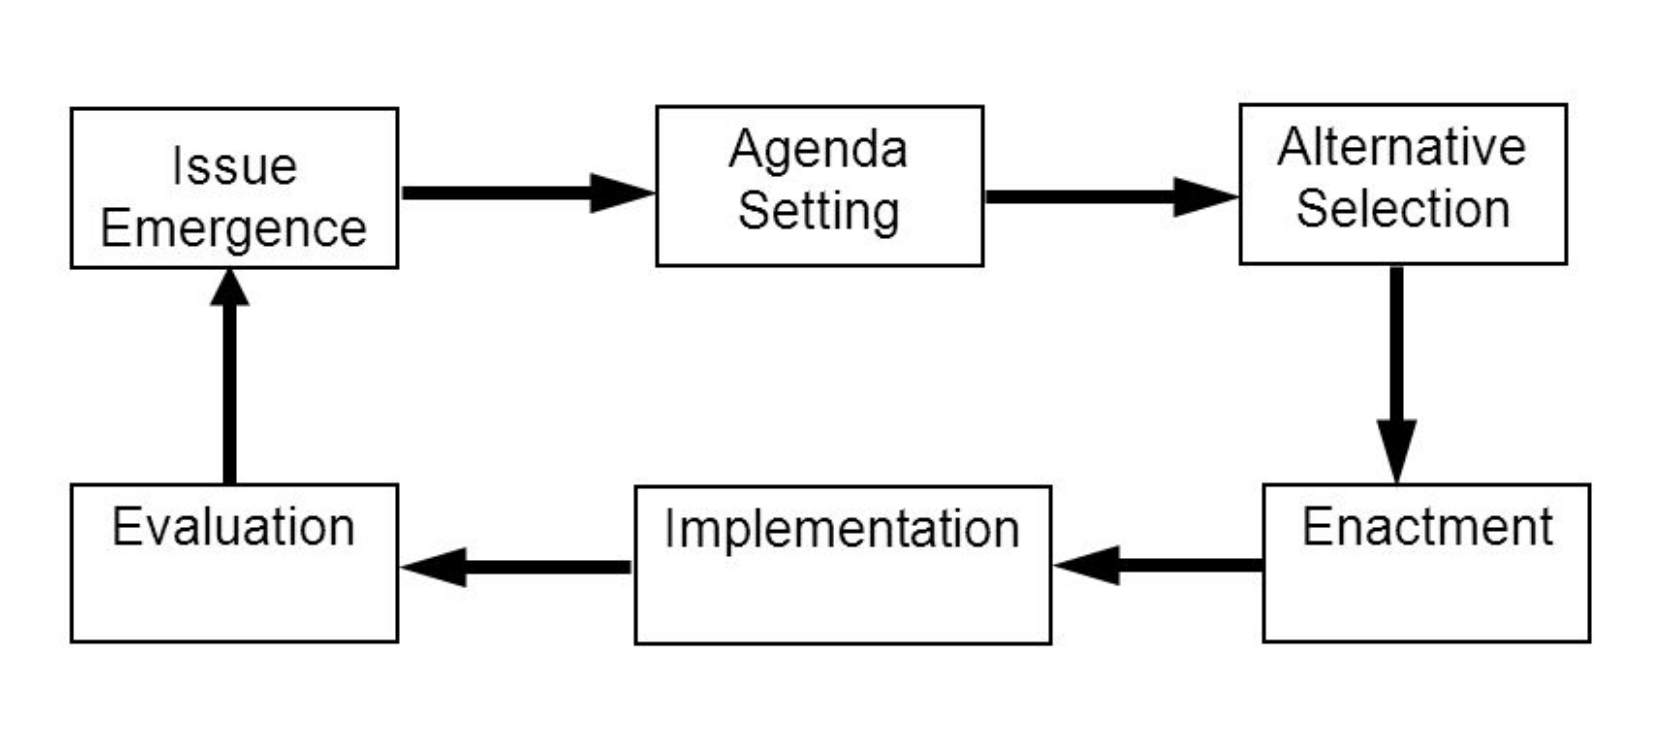
\includegraphics[scale=0.4]{policy_process_2.png}
%     \end{center}
%\end{frame}

%@@@@@@@@@@@@@@@@@@@@@@@@@@@@@@@@@@@@@@@@@@@@@@@@@
\begin{frame}
    \begin{center}
     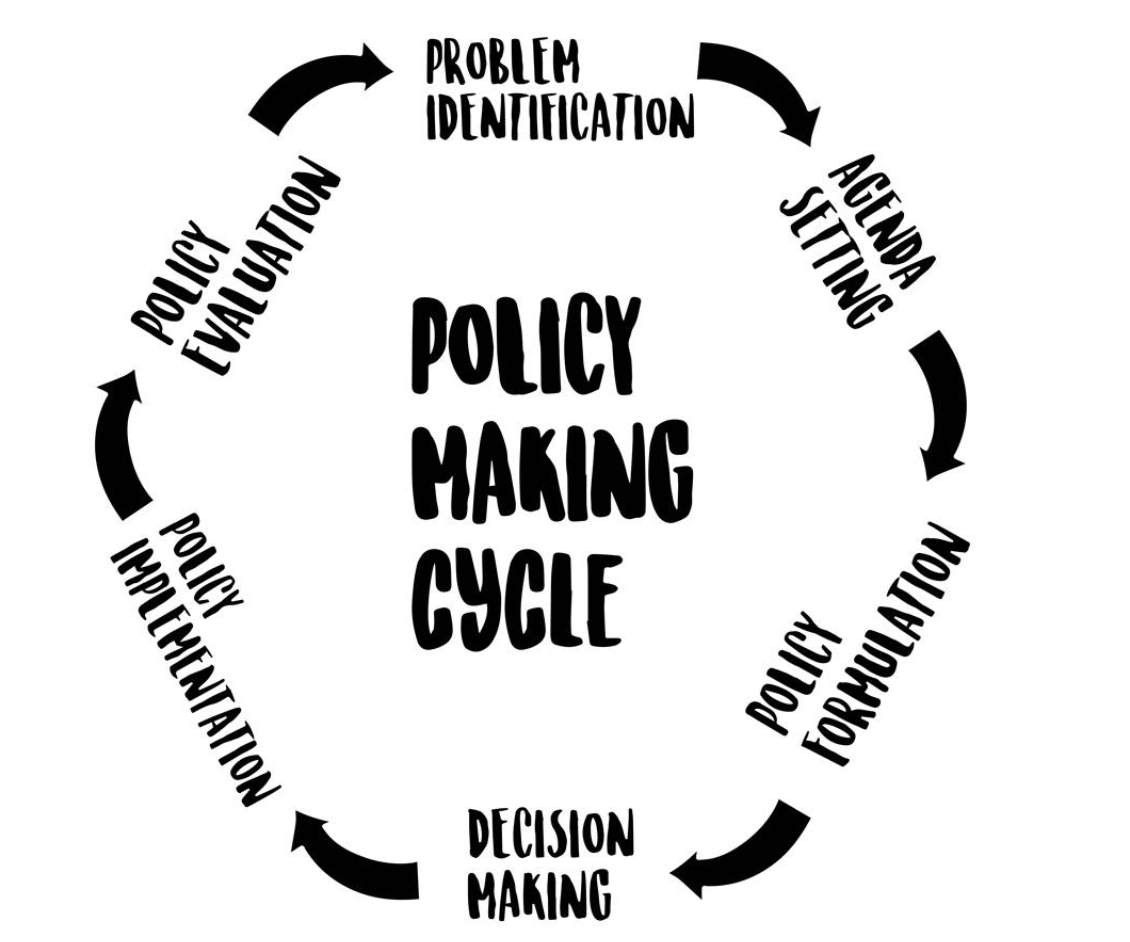
\includegraphics[scale=0.4]{policy_process.png}
     \end{center}
\end{frame}

%@@@@@@@@@@@@@@@@@@@@@@@@@@@@@@@@@@@@@@@@@@@@@@@@@
\begin{frame}
\frametitle{Input-Output Model}

\begin{itemize}
\item Input output modeling was originated by Leontief (1949);
\bigskip
\item  An \textbf{economic} approach: Leontief divided the US economy into 500 sectors, modeled each, and used a computer to solve the resulting system of equations;
\bigskip
\item Inputs are the various issues, pressures, information, and the like to which the actors in the system react;
\begin{itemize}
\item Generally: election results, public opinion, communications to elected officials and public managers, Interest group activity, news media;
%\item For congress: experts (e.g. CBO, GAO, CRS, and advisory panels), threat of presidential veto, threat of judicial review.
\end{itemize}
\bigskip
\item Outputs are public policy decisions.% -- statute law, case law, regulation.
\end{itemize}
\end{frame}

%@@@@@@@@@@@@@@@@@@@@@@@@@@@@@@@@@@@@@@@@@@@@@@@@@
\begin{frame}
\frametitle{Things that shape inputs: Structural Environment}
Structural environment = rules that dictate how government does business:
\bigskip
\begin{itemize}
\item<2-> Separation of powers;
\bigskip
\item<2-> Federalism;
\bigskip
\item<2-> Substantive policies: A policy that explains how the government will go about its policy goals in a particular area;
\bigskip
\item<2-> Procedural policies (e.g., Administrative Procedures Act);
\bigskip
\item<2-> Transparency requirements (Open public meetings laws, Freedom of Information Act).
\end{itemize}
\end{frame}

%@@@@@@@@@@@@@@@@@@@@@@@@@@@@@@@@@@@@@@@@@@@@@@@@@
\begin{frame}
\frametitle{Things that shape inputs: Social-Economic Environment}
Nature and composition of the population and its social structure:
\bigskip
\begin{itemize}
\item<2-> Demographics -- US has a greying population (tracked by e.g. the Census);
\bigskip
\item<2-> Race and ethnicity -- growth of minority groups;
\bigskip
\item<2-> Gender -- slightly more women than men;
\bigskip
\item<2-> Labor force participation -- workforce participation/unemployment (e.g. women's participation $\approx$ 60\%), income dynamics, immigration/assimilation, intermarriage;
\bigskip
\item<2-> Inequality, National Debt, Budget Deficit;
\end{itemize}
\end{frame}

%@@@@@@@@@@@@@@@@@@@@@@@@@@@@@@@@@@@@@@@@@@@@@@@@@
\begin{frame}
\frametitle{Things that shape inputs: Political Environment}
What is important/possible, the `national mood':
    \begin{center}
     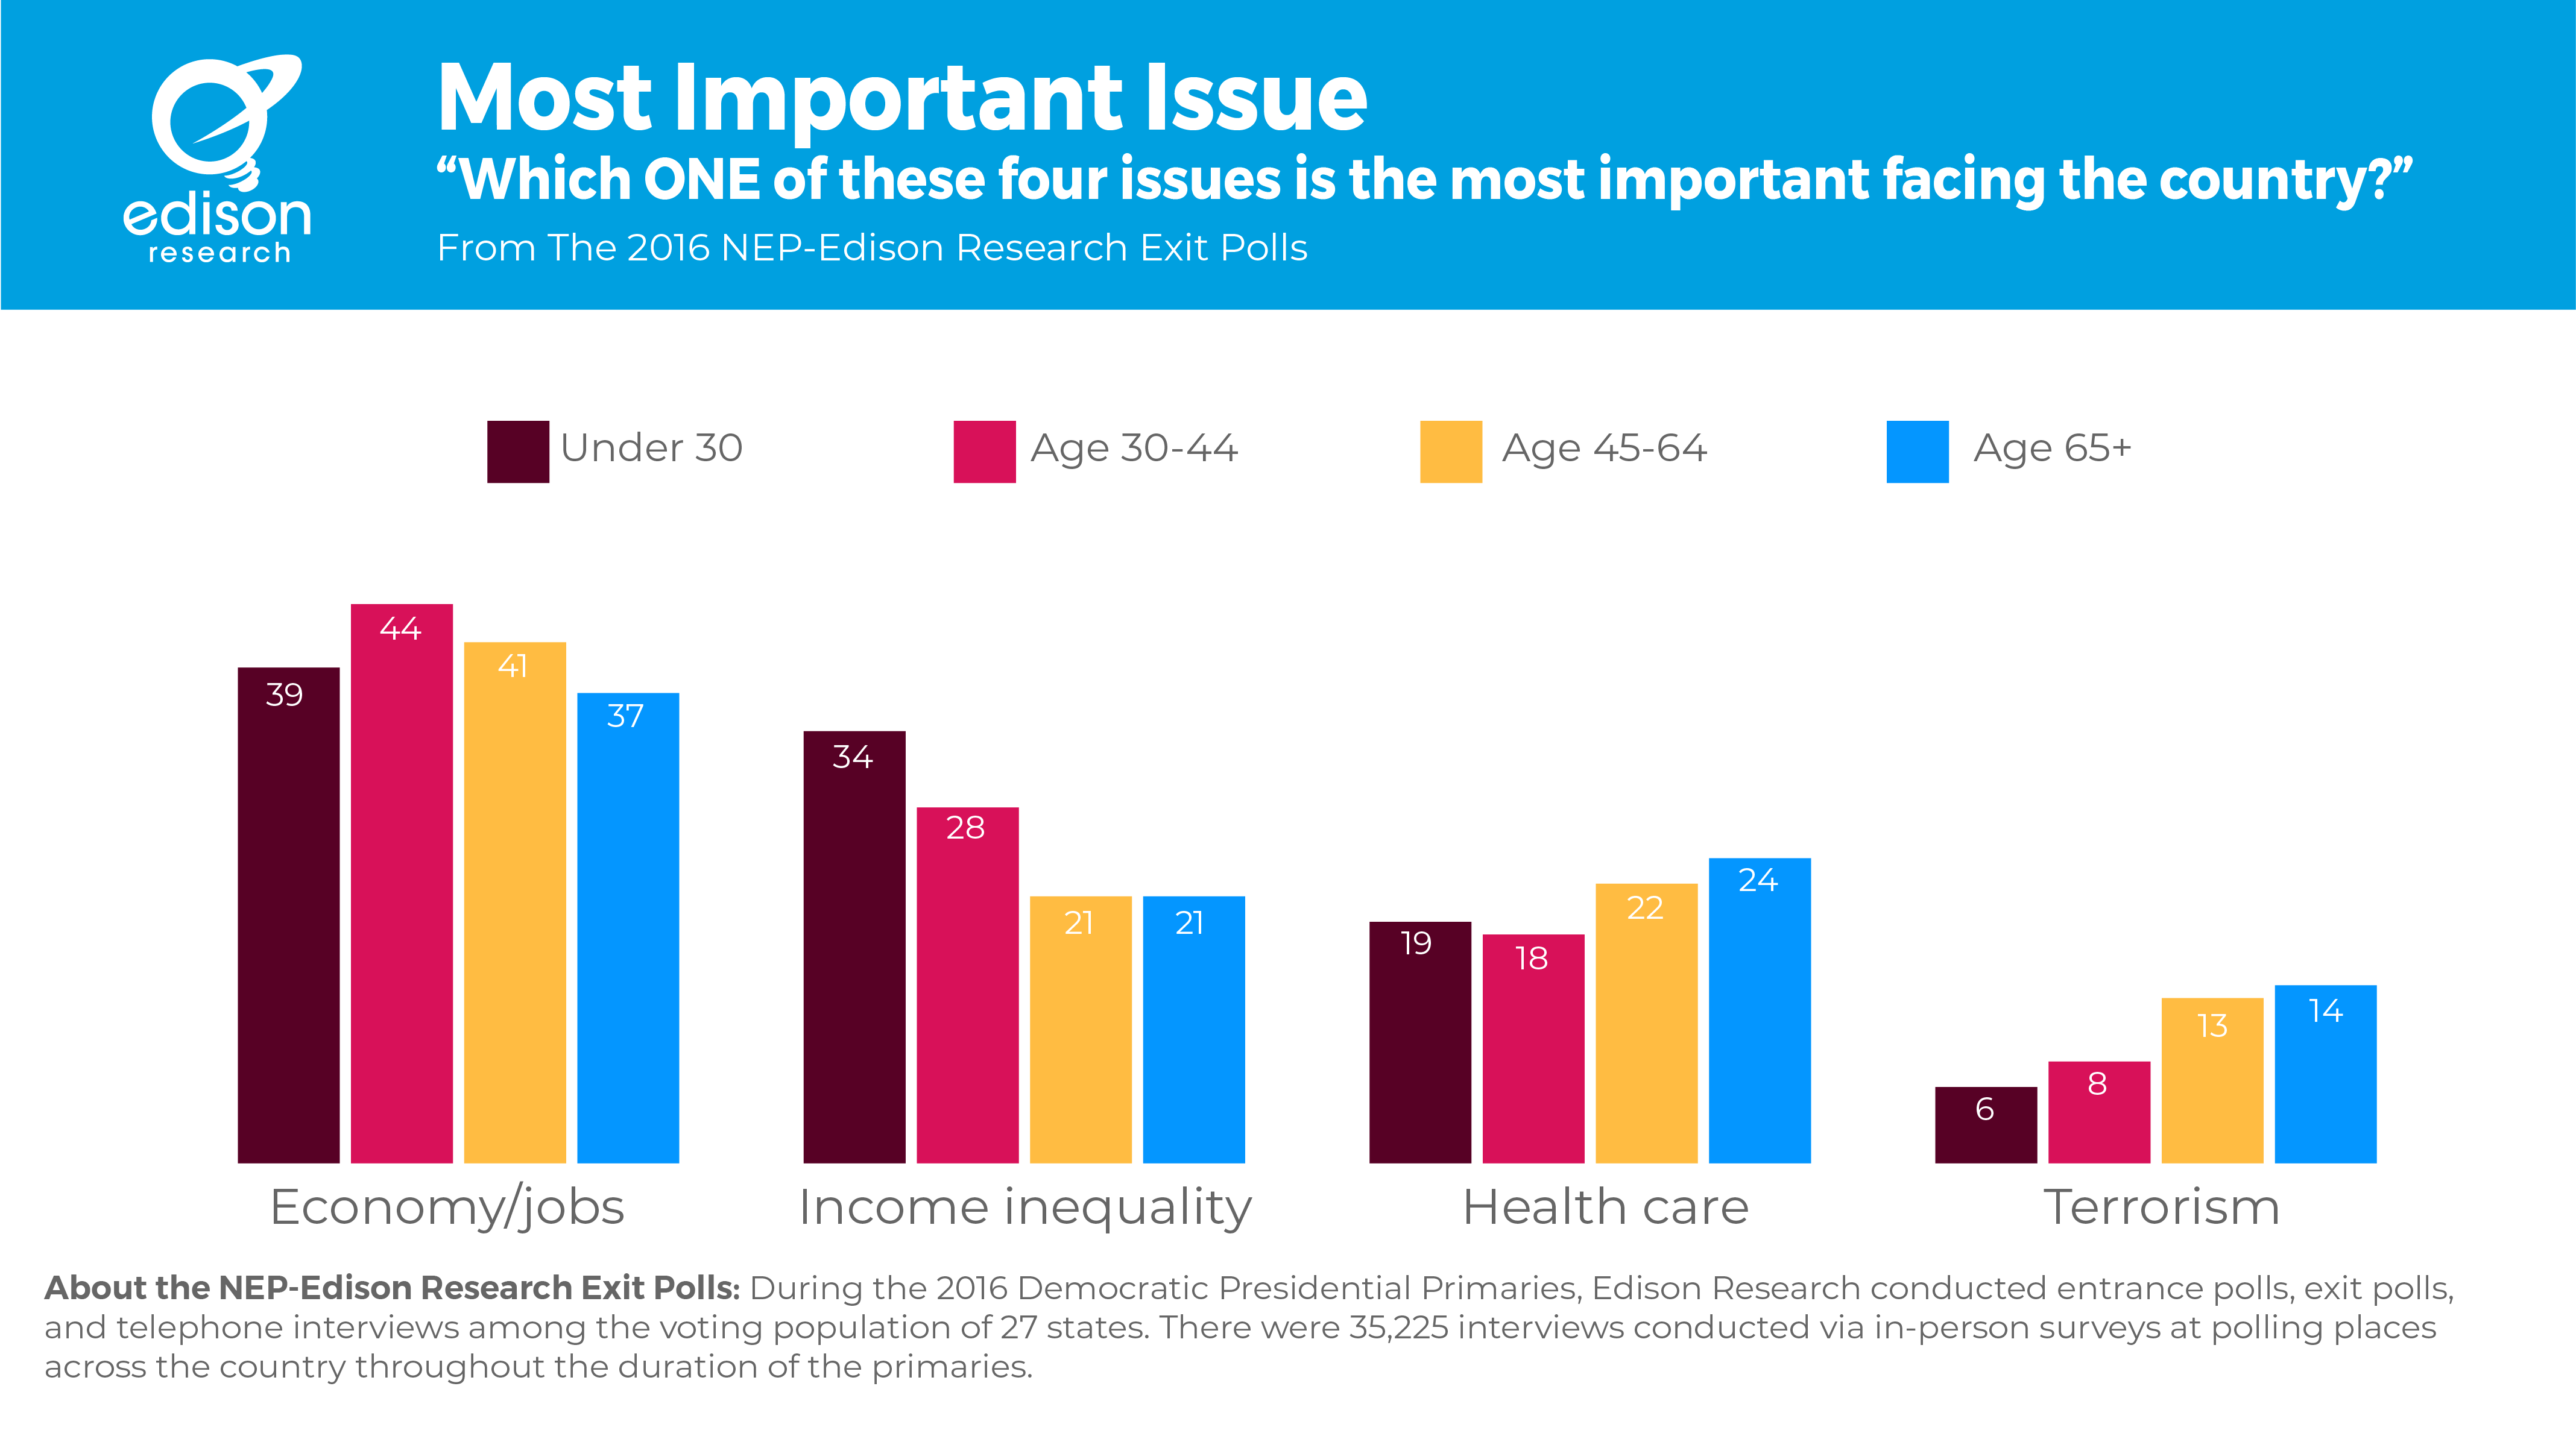
\includegraphics[scale=0.3]{mip.png}
     \end{center}

\end{frame}

%@@@@@@@@@@@@@@@@@@@@@@@@@@@@@@@@@@@@@@@@@@@@@@@@@
\begin{frame}
\frametitle{Things that shape inputs: Political Environment}
What is important/possible, the `national mood':
    \begin{center}
     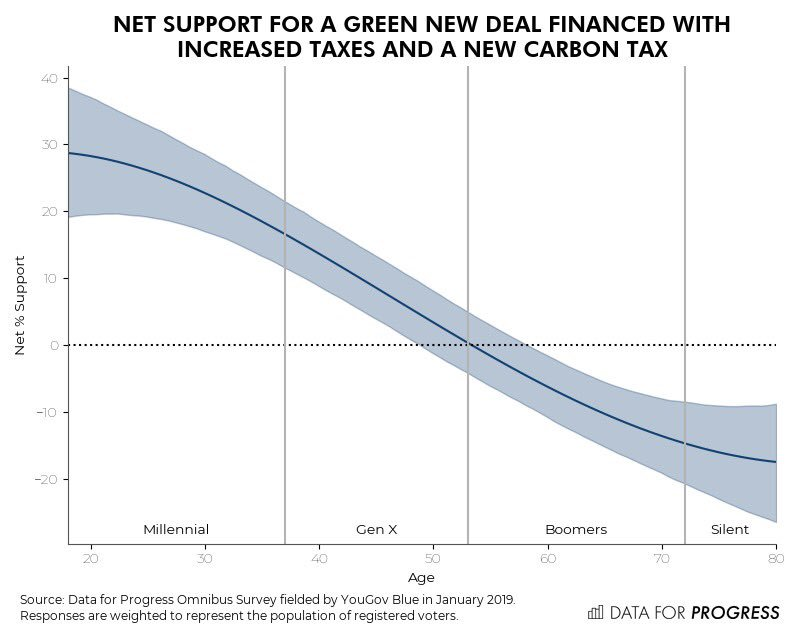
\includegraphics[scale=0.3]{age-gnd.jpeg}
     \end{center}

\end{frame}

%@@@@@@@@@@@@@@@@@@@@@@@@@@@@@@@@@@@@@@@@@@@@@@@@@
\begin{frame}
\frametitle{Things that shape inputs: Political Environment}
What is important/possible, the `national mood':
    \begin{center}
     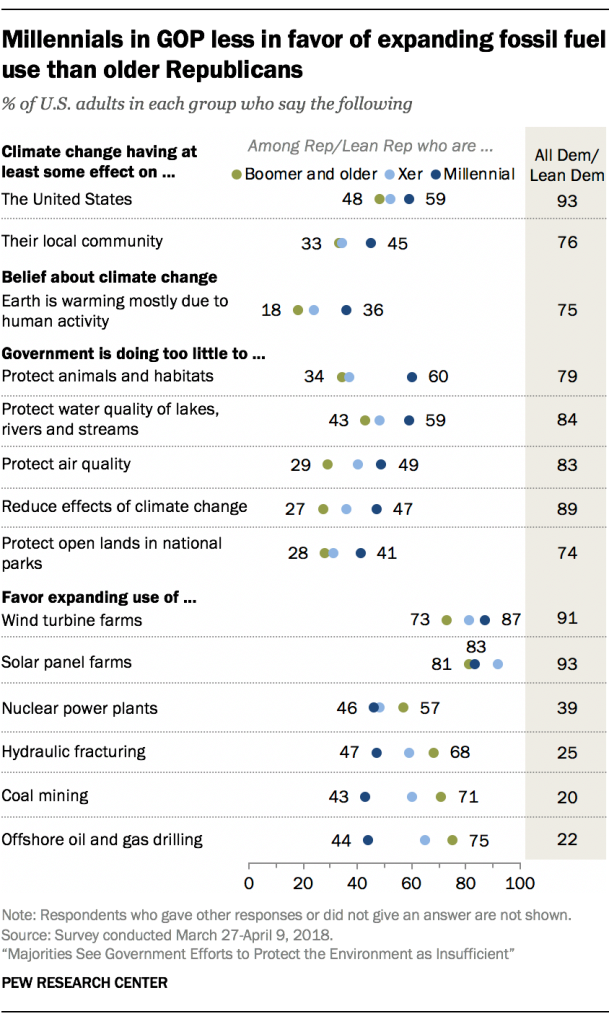
\includegraphics[scale=0.35]{cc-gop.png}
     \end{center}

\end{frame}

%%@@@@@@@@@@@@@@@@@@@@@@@@@@@@@@@@@@@@@@@@@@@@@@@@@
%\begin{frame}
%\frametitle{Things that shape inputs: Political Environment}
%What is important/possible, the `national mood':
%\bigskip
%\begin{itemize}
%\item HARD to measure... (presidential approval, right track questions, etc.);
%\bigskip
%\item Optimistic from end of WWII to 1963(ish);
%\bigskip
%\item Vietnam, Watergate, and inflation/unemployment soured the national mood;
%\bigskip
%\item Upbeat in early 2000s according to some measures.
%\end{itemize}
%\end{frame}



%%@@@@@@@@@@@@@@@@@@@@@@@@@@@@@@@@@@@@@@@@@@@@@@@@@
%\begin{frame}
%\frametitle{How do officials `process' inputs?}
%Where do policy priorities come from?  Policymakers, ultimately, who may be influenced by:
%\bigskip
%\begin{itemize}
%\item Crises - focusing events (e.g. COVID-19);
%\bigskip
%\bigskip
%\item Advisory Committees;
%\bigskip
%\bigskip
%\item Institutions designed to inform policy like the Congressional Budget Office (CBO), Congressional Research Service (CRS), and Government Accountability Office (GAO) and research arms of executive agencies (DARPA, IARPA, CIA, NOAA, etc.).
%\end{itemize}
%\end{frame}
%
%%@@@@@@@@@@@@@@@@@@@@@@@@@@@@@@@@@@@@@@@@@@@@@@@@@
%\begin{frame}
%\frametitle{How do officials `process' inputs?}
%    \begin{center}
%     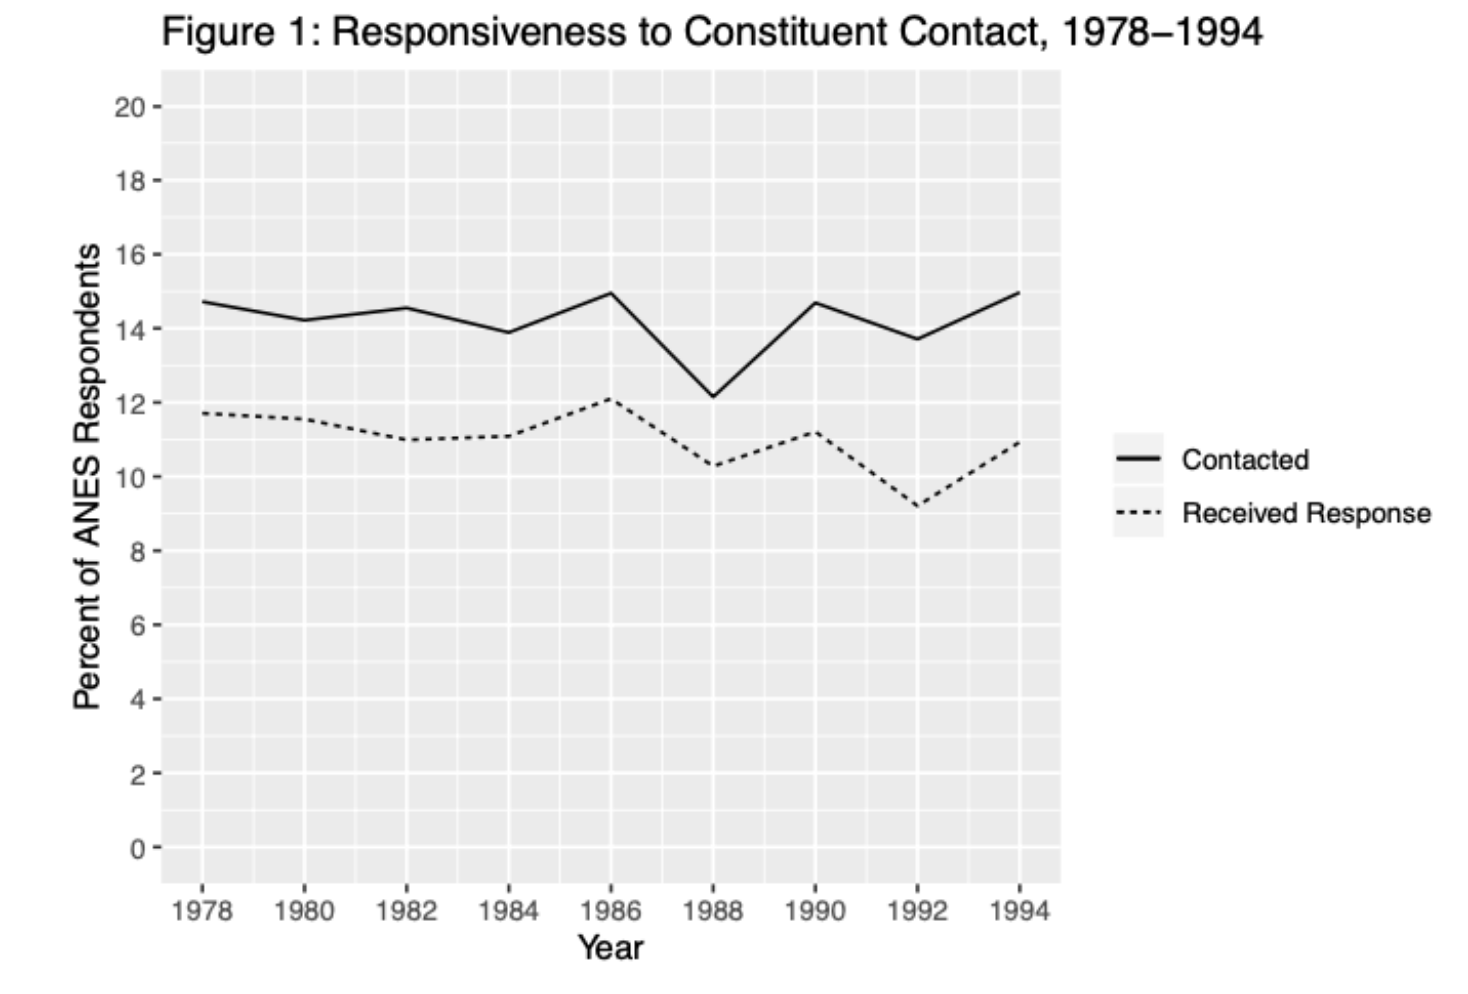
\includegraphics[scale=0.4]{responsiveness.png}
%     \end{center}
%
%\end{frame}
%
%%@@@@@@@@@@@@@@@@@@@@@@@@@@@@@@@@@@@@@@@@@@@@@@@@@
%\begin{frame}
%\frametitle{How do officials `process' inputs?}
%    \begin{center}
%     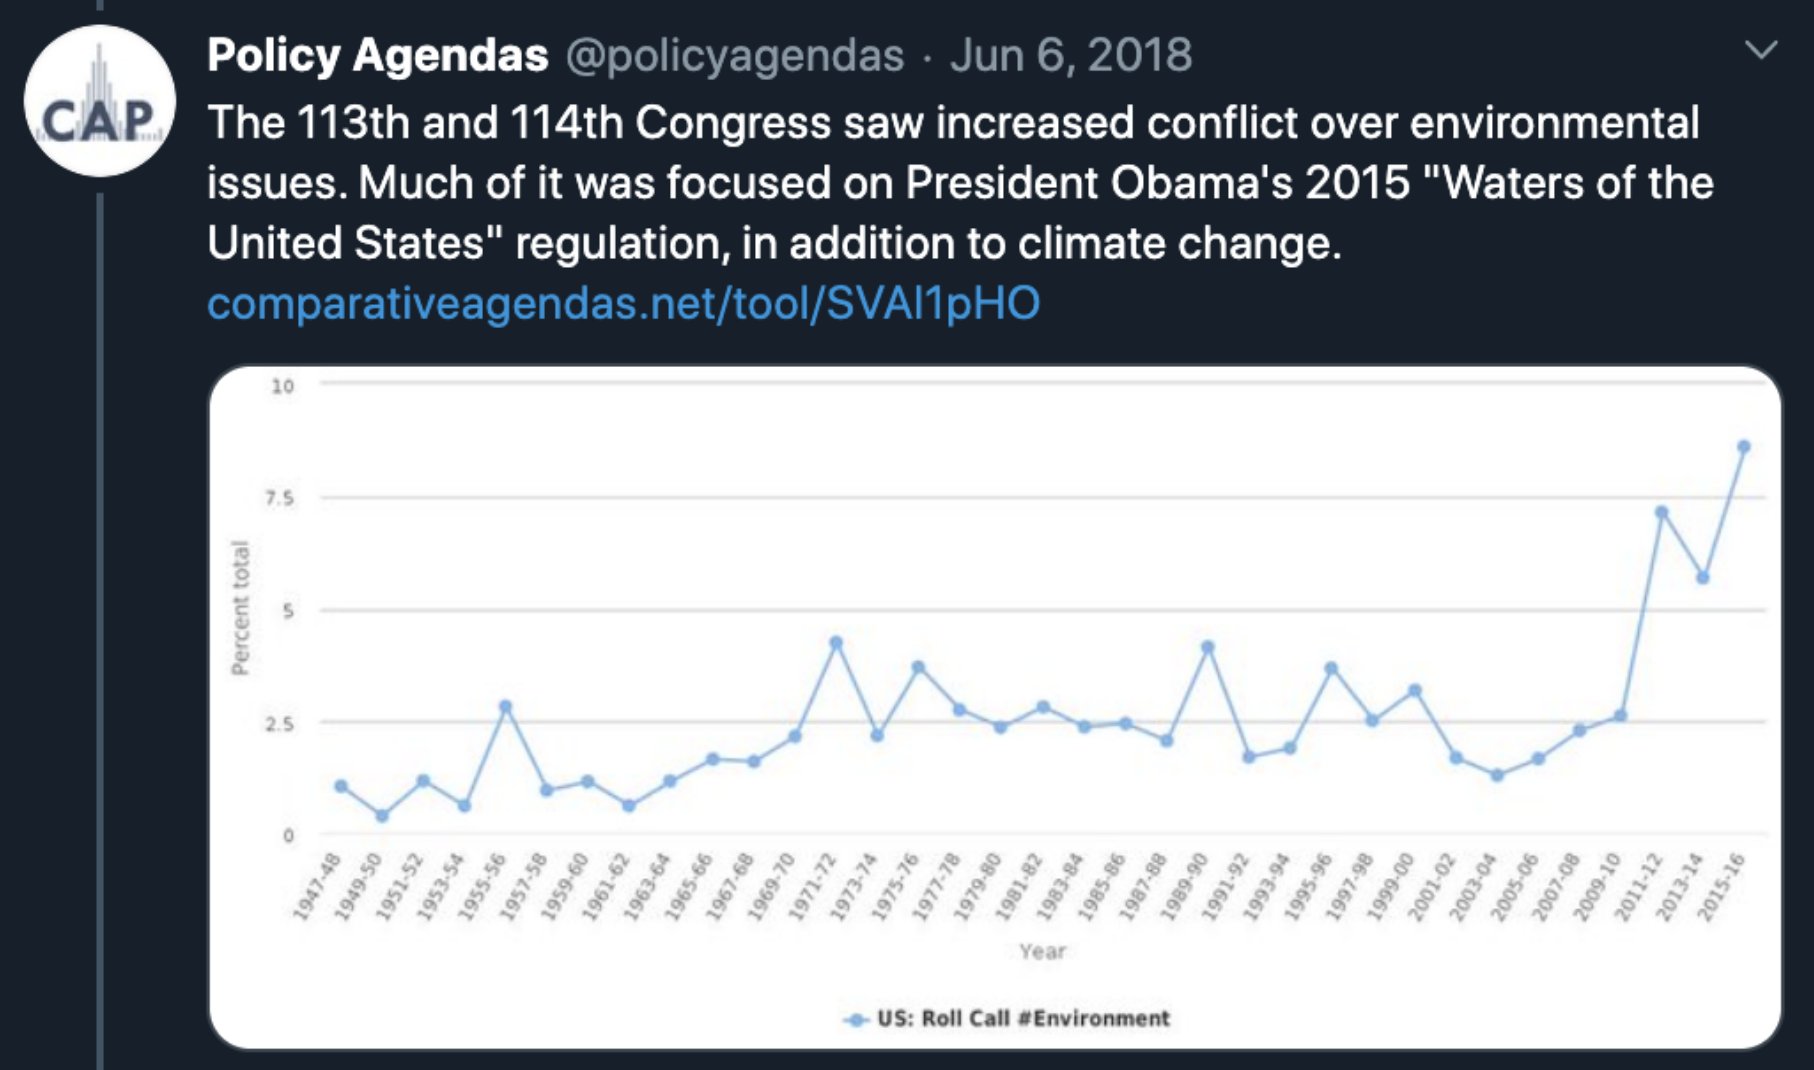
\includegraphics[scale=0.35]{congressional_votes.png}
%     \end{center}
%
%\end{frame}
%
%%@@@@@@@@@@@@@@@@@@@@@@@@@@@@@@@@@@@@@@@@@@@@@@@@@
%\begin{frame}
%\frametitle{Inputs for the Legislature}
%\begin{itemize}
%\item Casework (constituents);
%\bigskip
%\item Interest group pressure campaigns (constituents and non-constituents);
%\bigskip
%\item Experts (e.g. CBO, GAO, CRS, and advisory panels);
%\bigskip
%\item Media (often informed by experts or pressure campaigns);
%\bigskip
%\item Threat of presidential veto;
%\bigskip
%\item Threat of judicial review.
%\end{itemize}
%\end{frame}
%
%%@@@@@@@@@@@@@@@@@@@@@@@@@@@@@@@@@@@@@@@@@@@@@@@@@
%\begin{frame}
%\frametitle{Inputs for the Executive}
%Congressional oversight:
%\begin{itemize}
%\item Statutory deadlines, reporting requirements, or budget restrictions, the threat of repeal under the Congressional Review Act;
%\item CRS, CBO, GAO;
%\item Hearings and direct correspondence with legislators;
%\end{itemize}
%\bigskip
%Public comments on proposed agency rules (e.g., regulations.gov):
%\begin{itemize}
%\item Experts;
%\item Public pressure campaigns and other interest group lobbying coalitions.
%\end{itemize}
%
%\end{frame}
%
%%@@@@@@@@@@@@@@@@@@@@@@@@@@@@@@@@@@@@@@@@@@@@@@@@@
%\begin{frame}
%\frametitle{Inputs for the Executive}
%    \begin{center}
%     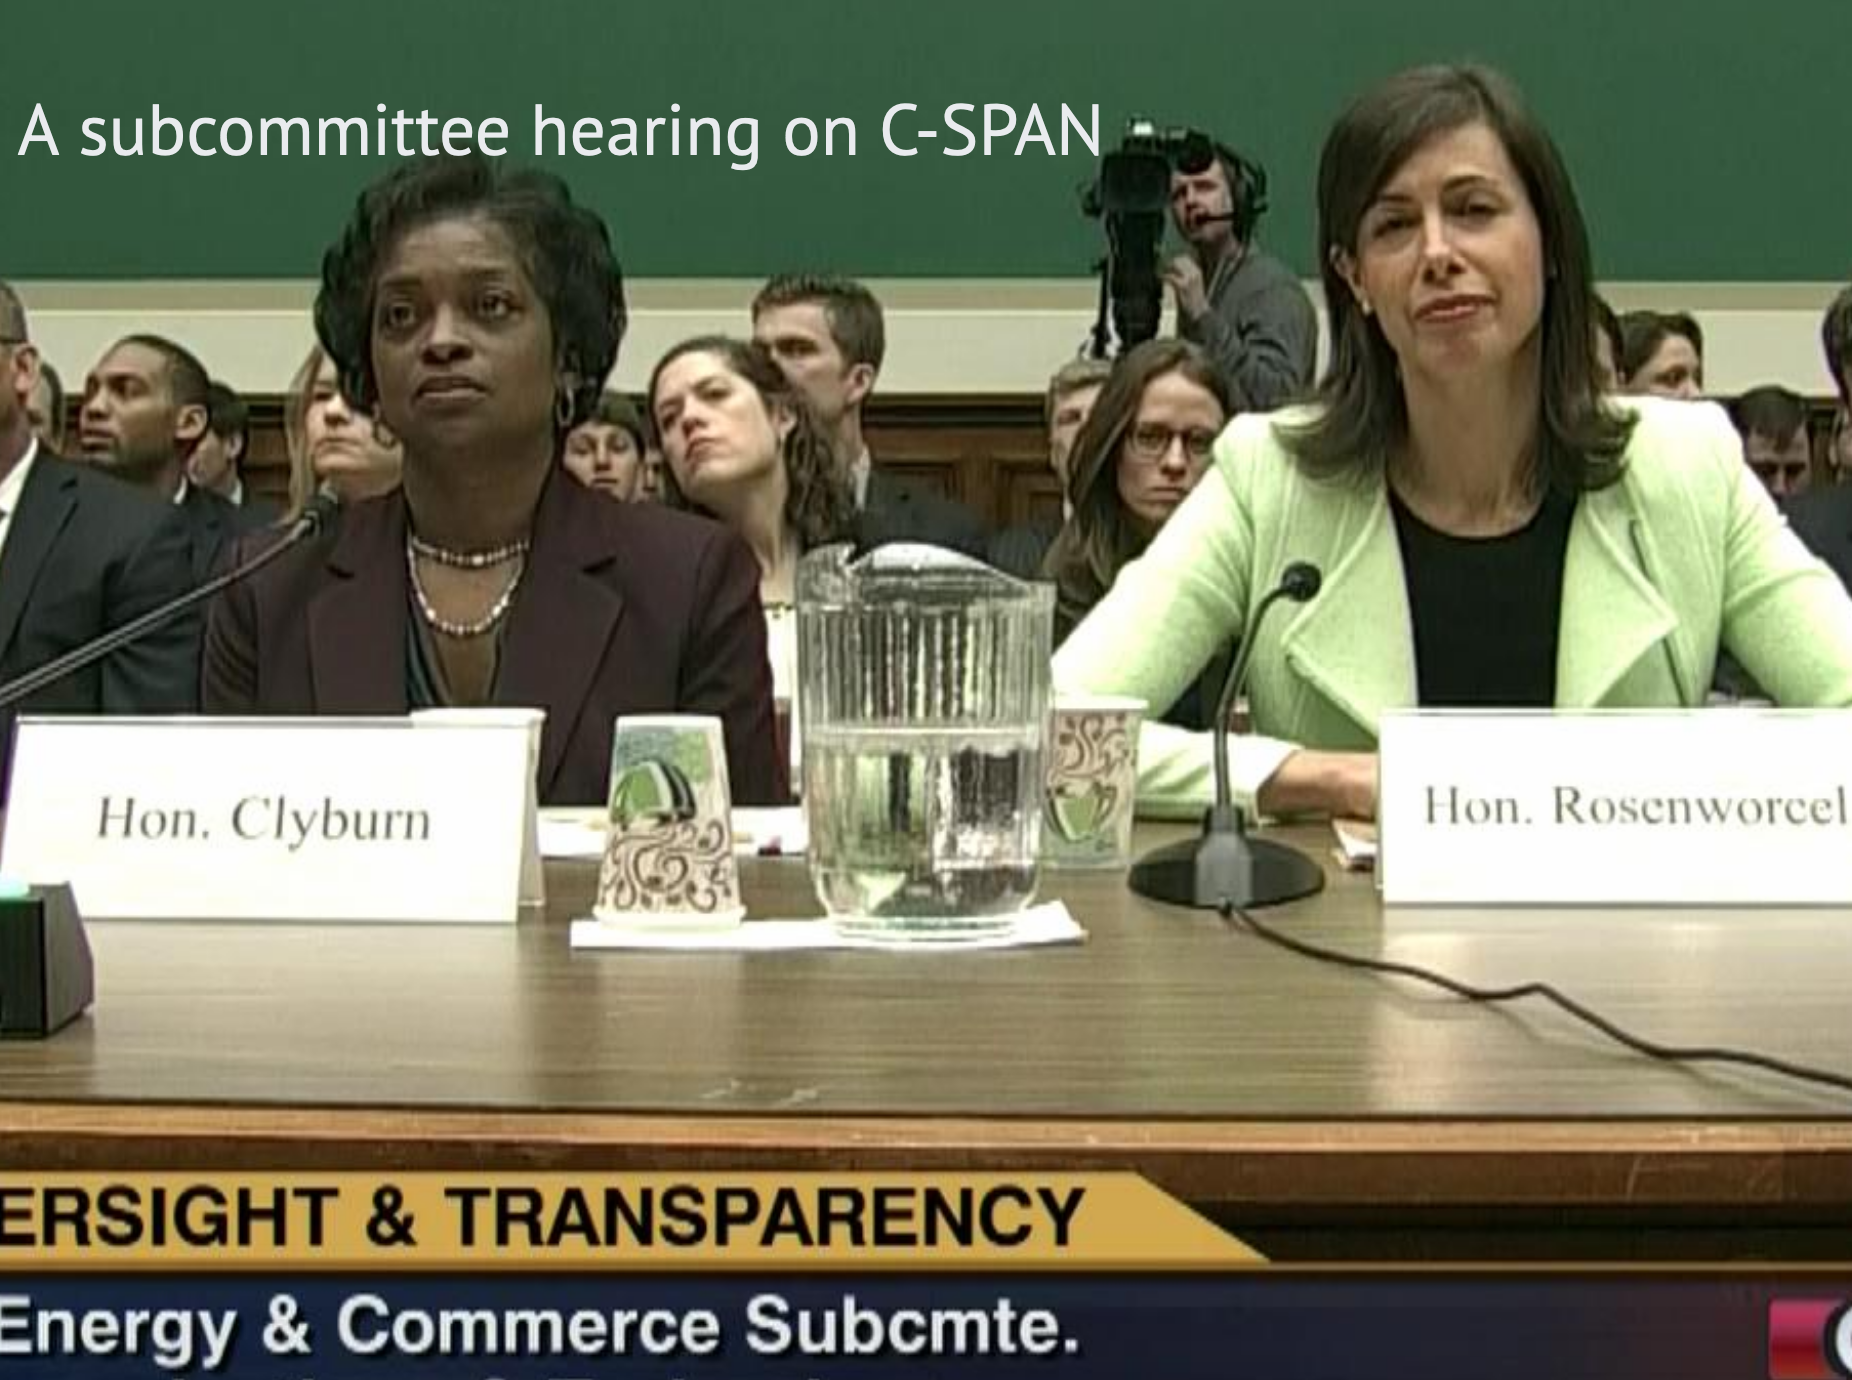
\includegraphics[scale=0.25]{hearing.png}
%     \end{center}
%
%
%\end{frame}
%
%%@@@@@@@@@@@@@@@@@@@@@@@@@@@@@@@@@@@@@@@@@@@@@@@@@
%\begin{frame}
%\frametitle{Inputs for the Judiciary}
%In selecting cases ("granting cert."):
%\begin{itemize}
%\item Original jurisdiction;
%\item Circuit splits (where a court has appellate jurisdiction);
%\item Test cases, where ``legal entrepreneurs" recruit sympathetic plaintiffs to change precedent;
%\end{itemize}
%
%In each case:
%\begin{itemize}
%\item Briefs (plaintiff, respondent, Solicitor General, amicus);
%\item Arguments (plaintiff, respondent and their designees);
%\end{itemize}
%
%The legal profession:
%\begin{itemize}
%\item Law Review articles;
%\end{itemize}
%
%Public opinion.
%\end{frame}

%@@@@@@@@@@@@@@@@@@@@@@@@@@@@@@@@@@@@@@@@@@@@@@@@@
\begin{frame}
\frametitle{Outputs are public policy decisions}
\begin{itemize}
\item \textbf{Statute laws}: Laws made by the legislature and signed by the executive, generally codified into The U.S. Code (e.g., Title 5 U.S. Code § 706) or state codes.
\bigskip
\item \textbf{Administrative rules}: Often called regulations, but also include funding criteria, deregulatory policy, and many other kinds of policy. They usually have the force of law, are published in the Federal Register (FR), and are codified in the Code of Federal Regulations (CFR) or state registers and codes (unlike informal guidance).
\bigskip
\item \textbf{Case law}: Interpretations of laws as a result of judicial decisions that influence future decisions, called legal precedent.
\end{itemize}
\end{frame}

%@@@@@@@@@@@@@@@@@@@@@@@@@@@@@@@@@@@@@@@@@@@@@@@@@
\begin{frame}
\begin{center}
\Huge \textbf{But what goes on in the middle?}
\end{center}
\end{frame}

%@@@@@@@@@@@@@@@@@@@@@@@@@@@@@@@@@@@@@@@@@@@@@@@@@
\begin{frame}
\begin{center}
\Huge \textbf{How do groups make decisions?}
\end{center}
\end{frame}

%@@@@@@@@@@@@@@@@@@@@@@@@@@@@@@@@@@@@@@@@@@@@@@@@@
\begin{frame}
\frametitle{A simple model of policy preferences}
\begin{itemize}
\item A spectrum of policy outcomes (e.g. a line with each point a policy);
\bigskip
\item A group of actors, each with an `ideal' policy (single peaked);
\bigskip
\item For each actor, utility that describes their `happiness' as we move away from their ideal policy;
\end{itemize}
    \begin{center}
     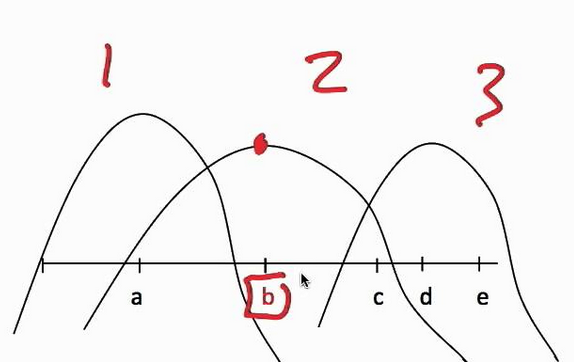
\includegraphics[scale=0.5]{sp.png}
     \end{center}
\end{frame}

%@@@@@@@@@@@@@@@@@@@@@@@@@@@@@@@@@@@@@@@@@@@@@@@@@
\begin{frame}
\frametitle{Median Voter Theorem}
\begin{itemize}
\item Can we offer predictions about what policy a group of rational actors will choose?
\bigskip
\bigskip
\item Median Voter Theorem: if preferences are single peaked and voting is by majority rule then there is a median voter and the winning alternative will be that preferred by the median voter.
\end{itemize}
    \begin{center}
     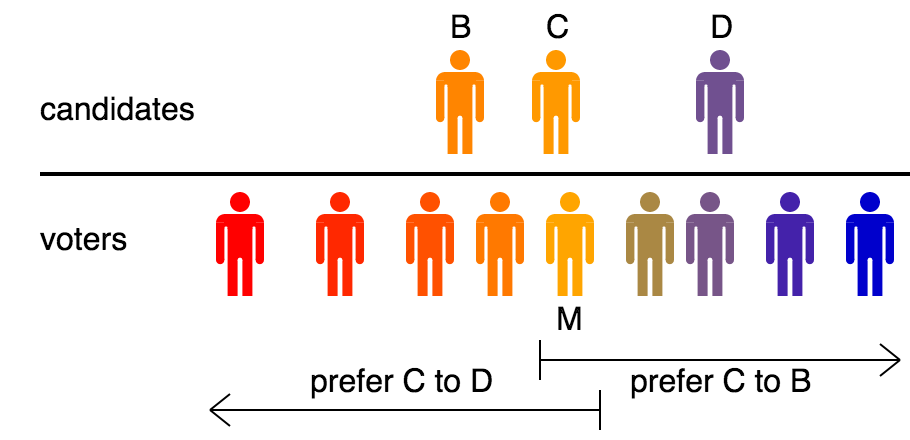
\includegraphics[scale=0.25]{Median_voter.png}
     \end{center}
\end{frame}

%@@@@@@@@@@@@@@@@@@@@@@@@@@@@@@@@@@@@@@@@@@@@@@@@@
\begin{frame}
\frametitle{Arrow's Impossibility Theorem}
\begin{itemize}
\item If a group of actors creates a group-ranking of alternatives how `rational' will their ranking be?
\bigskip
\bigskip
\item Imagine we have at least three alternatives ($x$, $y$, and $z$).  Some nice things we would like a group-ranking to do:
\begin{itemize}
\item \textbf{Unanimity}: if every actor likes $x$ more than $y$ then so should the group ranking;
\item \textbf{Independence of Irrelevant Alternatives (IIA)}: group ranking between $x$ and $y$ should only depend on individual rankings between $x$ and $y$ (i.e. $z$ should not matter);
\item \textbf{No-Dictatorship}: there is no actor such that if they like $x$ over $y$ then the group ranking must like $x$ over $y$;
\end{itemize}
\bigskip
\bigskip
\item Arrow's Theorem: If a group ranking satisfies unanimity and IIA then there must be a dictator.
\end{itemize}
\end{frame}



%@@@@@@@@@@@@@@@@@@@@@@@@@@@@@@@@@@@@@@@@@@@@@@@@@
\begin{frame}
\frametitle{Birkland$+$ Model of Policy}
\begin{itemize}
\item[] \color{white}Policy Domain: what substantive problems are under consideration (e.g. water pollution, defense, etc.)???
\begin{itemize}
\item[] \color{white}This specifies the actors involved (how are they organized?);
\item[] \color{white}Part of a policy regime;
\end{itemize}
\bigskip
\item \color{black}Input-output Model;
\begin{itemize}
\item Actors (e.g. legislature, regulators, etc.);
\item Inputs (e.g. institutional structure, demographics, national mood);
\item Black box decision making (structured by median voter thm, Arrow's thm);
\item Outputs (e.g. statute laws, rules, court decisions);
\end{itemize}
\bigskip
\item[] \color{white}Feedback and iteration.
\end{itemize}
\end{frame}

%@@@@@@@@@@@@@@@@@@@@@@@@@@@@@@@@@@@@@@@@@@@@@@@@@
\begin{frame}
\frametitle{Birkland$+$ Model of Policy}
\begin{itemize}
\item Policy Domain: what substantive problems are under consideration (e.g. water pollution, defense, etc.)???
\begin{itemize}
\item This specifies the actors involved (how are they organized?);
\item Part of a policy regime;
\end{itemize}
\bigskip
\item \color{black}Input-output Model;
\begin{itemize}
\item Actors (e.g. legislature, regulators, etc.);
\item Inputs (e.g. institutional structure, demographics, national mood);
\item Black box decision making (structured by median voter thm, Arrow's thm);
\item Outputs (e.g. statute laws, rules, court decisions);
\end{itemize}
\bigskip
\item[] \color{white}Feedback and iteration.
\end{itemize}
\end{frame}

%@@@@@@@@@@@@@@@@@@@@@@@@@@@@@@@@@@@@@@@@@@@@@@@@@
\begin{frame}
\frametitle{Birkland$+$ Model of Policy}
\begin{itemize}
\item Policy Domain: what substantive problems are under consideration (e.g. water pollution, defense, etc.)???
\begin{itemize}
\item This specifies the actors involved (how are they organized?);
\item Part of a policy regime;
\end{itemize}
\bigskip
\item \color{black}Input-output Model;
\begin{itemize}
\item Actors (e.g. legislature, regulators, etc.);
\item Inputs (e.g. institutional structure, demographics, national mood);
\item Black box decision making (structured by median voter thm, Arrow's thm);
\item Outputs (e.g. statute laws, rules, court decisions);
\end{itemize}
\bigskip
\item Feedback and iteration.
\end{itemize}
\end{frame}




%%@@@@@@@@@@@@@@@@@@@@@@@@@@@@@@@@@@@@@@@@@@@@@@@@@
%\begin{frame}
%\frametitle{Stability}
%\begin{itemize}
%\item Divided Power (1787 - 1870) -- period of institutionalization;
%\bigskip
%\bigskip
%\item State Activism (1870 - 1933) -- reaction to aggregation of economic power into monopolies;
%\bigskip
%\bigskip
%\item National Activism (1933 - 1961) -- reaction to depression and World War;
%\bigskip
%\bigskip
%\item National Standards (1961 - ???) -- reaction to ongoing social justice shortfalls.
%\end{itemize}
%\end{frame}
%
%%@@@@@@@@@@@@@@@@@@@@@@@@@@@@@@@@@@@@@@@@@@@@@@@@@
%\begin{frame}
%\frametitle{Stability}
%\begin{itemize}
%\item Has ideological, political, and policy flavors;
%\bigskip
%\bigskip
%\item Is derived from norms and rules (e.g. filibuster);
%\bigskip
%\bigskip
%\item Fragmentation (between branches, between federal and state levels);
%\bigskip
%\bigskip
%\item Is it good or bad?
%\end{itemize}
%\end{frame}

%@@@@@@@@@@@@@@@@@@@@@@@@@@@@@@@@@@@@@@@@@@@@@@@@@
\begin{frame}
\begin{center}
\Huge\textbf{Actors, official and unofficial}
\end{center}
\end{frame}

%@@@@@@@@@@@@@@@@@@@@@@@@@@@@@@@@@@@@@@@@@@@@@@@@@
\begin{frame}
\frametitle{Official Actors}
\begin{center}
\Large \textbf{A participant in the policy process whose involvement is motivated or mandated by their official position in a government agency or office.}
\end{center}
\end{frame}

%@@@@@@@@@@@@@@@@@@@@@@@@@@@@@@@@@@@@@@@@@@@@@@@@@
\begin{frame}
\frametitle{Official Actors}
\begin{itemize}
\item Legislature (and staff);
\bigskip
\bigskip
\item Executive (and staff);
\bigskip
\bigskip
\item Career civil service, i.e. bureaucrats;
\bigskip
\bigskip
\item Judges;
\end{itemize}
\end{frame}

%@@@@@@@@@@@@@@@@@@@@@@@@@@@@@@@@@@@@@@@@@@@@@@@@@
\begin{frame}
\frametitle{Legislature (and staff)}
\begin{itemize}
\item Major job: make statute law:
\begin{itemize}
\item Bills, public or private - general issues or of concern to individuals, have force of law;
\item Joint resolutions - temporary matters, have force of law;
\item Concurrent resolutions - limited to use for expressing facts, doing congressional business, etc., no force of law.
\end{itemize}
\bigskip
\item Casework - helping constituents;
\bigskip
\item Oversight - supervision of executive branch implementation of laws;
\begin{itemize}
\item Hearings for information, revelation, and political pointmaking;
\item GAO/CRS;
\item Media/constituents;
\end{itemize}
\bigskip
\item Organization is decentralized, bulk of work is done in committees -- can make BIG policies difficult to create.
\end{itemize}
\end{frame}

%@@@@@@@@@@@@@@@@@@@@@@@@@@@@@@@@@@@@@@@@@@@@@@@@@
\begin{frame}
\frametitle{Executive (and staff)}
\begin{itemize}
\item Major job: implement laws, check legislature with veto, create focus;
\bigskip
\item Policymaking advantages:
\begin{itemize}
\item Veto is an incredibly powerful weapon for conservative policymaking;
\item Organization is centralized;
\item Informational advantage - executive branch knows how laws are being administered because they do it (CBO/committee staff a reaction to this);
\end{itemize}
\bigskip
\item Policymaking Disadvantages:
\begin{itemize}
\item Major power is `power to persuade' (e.g. agenda setting);
\item Expansive administrative responsibility - must delegate;
\end{itemize}
\end{itemize}
\end{frame}

%@@@@@@@@@@@@@@@@@@@@@@@@@@@@@@@@@@@@@@@@@@@@@@@@@
\begin{frame}
\frametitle{Career civil service, i.e. bureaucrats}
\begin{itemize}
\item Rule based power to give orders;
\bigskip
\item Hierarchical;
\bigskip
\item Expertise;
\bigskip
\item SOPs.
\end{itemize}
\end{frame}

%@@@@@@@@@@@@@@@@@@@@@@@@@@@@@@@@@@@@@@@@@@@@@@@@@
\begin{frame}
\frametitle{Career civil service, i.e. bureaucrats}
\begin{itemize}
\item Major job: provide public goods, implement laws;
\bigskip
\item Does bureaucracy \textbf{make} policy?
\begin{itemize}
\item Choices without explicit instruction from Congress;
\item Bureaucratic discretion (does this help Congress?);
\end{itemize}
\bigskip
\item How do we hold bureaucrats accountable?
\begin{quote}
The amount of discretion accorded an agency is a function of its resources (expertise, cohesion, legislative authority, policy salience, and leadership) and the tolerances of other actors in the political system. Each actor has a zone of acceptance; and if agency decisions fall within that zone, no action will be taken.
\end{quote}
\item Competition between bureaucracies captured differently.
\end{itemize}
\end{frame}

%@@@@@@@@@@@@@@@@@@@@@@@@@@@@@@@@@@@@@@@@@@@@@@@@@
\begin{frame}
\frametitle{Judges}
\begin{itemize}
\item Major job: interpret the law, judicial review;
\bigskip
\item Both the weakest and strongest of branches:
\begin{itemize}
\item Lacks `either the sword or the purse' -- cannot tax and spend or impose via force;
\item Cannot control agenda;
\item Final arbiter on meaning of law;
\end{itemize}
\bigskip
\item Sets the boundary of acceptable policies:
\begin{itemize}
\item e.g. Plessy v. Ferguson and Brown v. Board of Education;
\item Dispute resolution;
\item Application of laws to new situations.
\end{itemize}
\bigskip
\item `law was not what the legislature ordered but what the courts decided in concrete cases.'
\end{itemize}
\end{frame}

%@@@@@@@@@@@@@@@@@@@@@@@@@@@@@@@@@@@@@@@@@@@@@@@@@
\begin{frame}
\frametitle{Birkland$+$ Model of Policy}
\begin{itemize}
\item Policy Domain: what substantive problems are under consideration (e.g. water pollution, defense, etc.)???
\begin{itemize}
\item This specifies the actors involved (how are they organized?);
\item Part of a policy regime;
\end{itemize}
\bigskip
\item \color{black}Input-output Model;
\begin{itemize}
\item Actors (e.g. legislature, regulators, etc.);
\item Inputs (e.g. institutional structure, demographics, national mood);
\item Black box decision making (structured by median voter thm, Arrow's thm);
\item Outputs (e.g. statute laws, rules, court decisions);
\end{itemize}
\bigskip
\item Feedback and iteration.
\end{itemize}
\end{frame}

%@@@@@@@@@@@@@@@@@@@@@@@@@@@@@@@@@@@@@@@@@@@@@@@@@
\begin{frame}
\frametitle{Birkland$+$ Model of Policy}
\begin{itemize}
\item Policy Domain: what substantive problems are under consideration (e.g. water pollution, defense, etc.)???  This specifies:
\begin{itemize}
\item The actors involved, \textbf{official actors who can make decisions $+$ stakeholders;} 
\item \textbf{Their organization, e.g. iron triangle, policy community;}
\end{itemize} 
\bigskip
\item \color{black}Input-output Model;
\begin{itemize}
\item Actors: \textbf{legislature, executive, bureaucrats, justices and the available levers;}
\item Inputs (e.g. institutional structure, demographics, national mood);
\item Black box decision making (structured by median voter thm, Arrow's thm);
\item Outputs (e.g. statute laws, rules, court decisions);
\end{itemize}
\bigskip
\item Feedback and iteration.
\end{itemize}
\end{frame}

%@@@@@@@@@@@@@@@@@@@@@@@@@@@@@@@@@@@@@@@@@@@@@@@@@
\begin{frame}
\begin{center}
\Huge \textbf{What should these official actors do???}
\end{center}
\end{frame}

%@@@@@@@@@@@@@@@@@@@@@@@@@@@@@@@@@@@@@@@@@@@@@@@@@
\begin{frame}
\begin{center}
\Huge Agenda Setting
\end{center}
\end{frame}

%@@@@@@@@@@@@@@@@@@@@@@@@@@@@@@@@@@@@@@@@@@@@@@@@@
\begin{frame}
\frametitle{Agenda}
\begin{center}
\Large The list of things being discussed and sometimes acted upon by an institution, the news media, or the public at large.
\end{center}
\end{frame}

%@@@@@@@@@@@@@@@@@@@@@@@@@@@@@@@@@@@@@@@@@@@@@@@@@
\begin{frame}
\frametitle{Agenda Setting}
\begin{center}
\Large Agenda setting is the process by which problems and alternative solutions gain or lose public and elite attention.
\end{center}
\end{frame}

%@@@@@@@@@@@@@@@@@@@@@@@@@@@@@@@@@@@@@@@@@@@@@@@@@
\begin{frame}
\frametitle{Agenda Setting}
\begin{itemize}
\item Agenda universe -- all possible ideas;
\bigskip
\bigskip
\item Systemic agenda -- all possible ideas that could be considered by participants in the policy process;
\bigskip
\bigskip
\item Institutional agenda -- list of issues currently considered by a governmental institution;
\bigskip
\bigskip
\item Decision agenda -- the things about to be acted upon by a governmental institution;
\end{itemize}
\end{frame}

%@@@@@@@@@@@@@@@@@@@@@@@@@@@@@@@@@@@@@@@@@@@@@@@@@
\begin{frame}
\frametitle{Faces of Power}
\begin{itemize}
\item the ability to compel people to do things against their will;
\begin{itemize}
\item A makes decisions that affect B;
\item e.g. authoritarianism, prisoners, children;
\end{itemize}
\bigskip
\item the ability prevent people from doing things they want to do;
\begin{itemize}
\item A prevents B from raising issues;
\item e.g. environmentalism;
\end{itemize}
\end{itemize}
\bigskip
``All forms of political organization have a bias in favor of the exploitation of some kinds of conflict and the suppression of others because \textbf{organization is the mobilization of bias}. Some issues are organized into politics while others are organized out." -- E.E. Schattschneider

\end{frame}

%@@@@@@@@@@@@@@@@@@@@@@@@@@@@@@@@@@@@@@@@@@@@@@@@@
\begin{frame}
\frametitle{Social Construction}
\begin{itemize}
\item \textbf{Social construction} = the process by which issues and problems are defined in society, groups that win this level often win at the policy level too;
\bigskip
\item Example: is the issue a \textbf{condition} or a \textbf{problem}?
\bigskip
\item Example: is the problem about \textbf{public goods} provision or \textbf{private goods} provision?
\bigskip
\item Example: is drunk driving a problem of individual responsibility or of transportation shortfalls?
\bigskip
\item Example: is gun violence reduction about gun control or about mental health?
\end{itemize}
\end{frame}

%@@@@@@@@@@@@@@@@@@@@@@@@@@@@@@@@@@@@@@@@@@@@@@@@@
\begin{frame}
\frametitle{Birkland$+$ Model of Policy}
\begin{itemize}
\item Policy Domain: what substantive problems are under consideration (e.g. water pollution, defense, etc.)???  This specifies:
\begin{itemize}
\item The actors involved, official actors who can make decisions $+$ stakeholders; 
\item Their organization, e.g. iron triangle, policy community;
\end{itemize} 
\bigskip
\item \color{black}Input-output Model;
\begin{itemize}
\item Actors: legislature, executive, bureaucrats, justices and the available levers;
\item Inputs (e.g. institutional structure, demographics, national mood);
\item Black box decision making (structured by median voter thm, Arrow's thm);
\item Outputs (e.g. statute laws, rules, court decisions);
\end{itemize}
\bigskip
\item Feedback and iteration.
\end{itemize}
\end{frame}

%@@@@@@@@@@@@@@@@@@@@@@@@@@@@@@@@@@@@@@@@@@@@@@@@@
\begin{frame}
\frametitle{Birkland$+$ Model of Policy}
\begin{itemize}
\item Policy Domain: what substantive problems are under consideration (e.g. water pollution, defense, etc.)???  This specifies:
\begin{itemize}
\item The actors involved, official actors who can make decisions $+$ stakeholders; 
\item Their organization, e.g. iron triangle, policy community;
\item \textbf{the systemic agenda;}
\end{itemize}
\bigskip
\item \color{black}Input-output Model;
\begin{itemize}
\item Actors: legislature, executive, bureaucrats, justices and the available levers;
\item Inputs: \textbf{agenda setting (application of power/social construction) specifies the institutional and decision agendas;}
\item Black box decision making (structured by median voter thm, Arrow's thm) \textbf{works on the decision agenda;}
\item Outputs (e.g. statute laws, rules, court decisions);
\end{itemize}
\bigskip
\item Feedback and iteration.
\end{itemize}
\end{frame}

%@@@@@@@@@@@@@@@@@@@@@@@@@@@@@@@@@@@@@@@@@@@@@@@@@
\begin{frame}
\begin{center}
\Huge \textbf{When does policy change happen???}
\end{center}
\end{frame}

%@@@@@@@@@@@@@@@@@@@@@@@@@@@@@@@@@@@@@@@@@@@@@@@@@
\begin{frame}
\frametitle{Weapons of the weak}
\begin{columns}

\begin{column}{0.5\textwidth}

\begin{itemize}
\item How do groups break the policy monopoly?
\begin{itemize}
\item Expand the scope of conflict;
\item Appeal to a high level;
\end{itemize}
\bigskip
\item How does policy change happen once the policy monopoly is broken?
\begin{itemize}
\item Political stream -- e.g. electoral change;
\item Problem stream -- e.g. problem definition change;
\item Policy stream -- e.g. articulation of better policies;
\end{itemize}
\end{itemize}
\end{column}
\begin{column}{0.5\textwidth}
    \begin{center}
     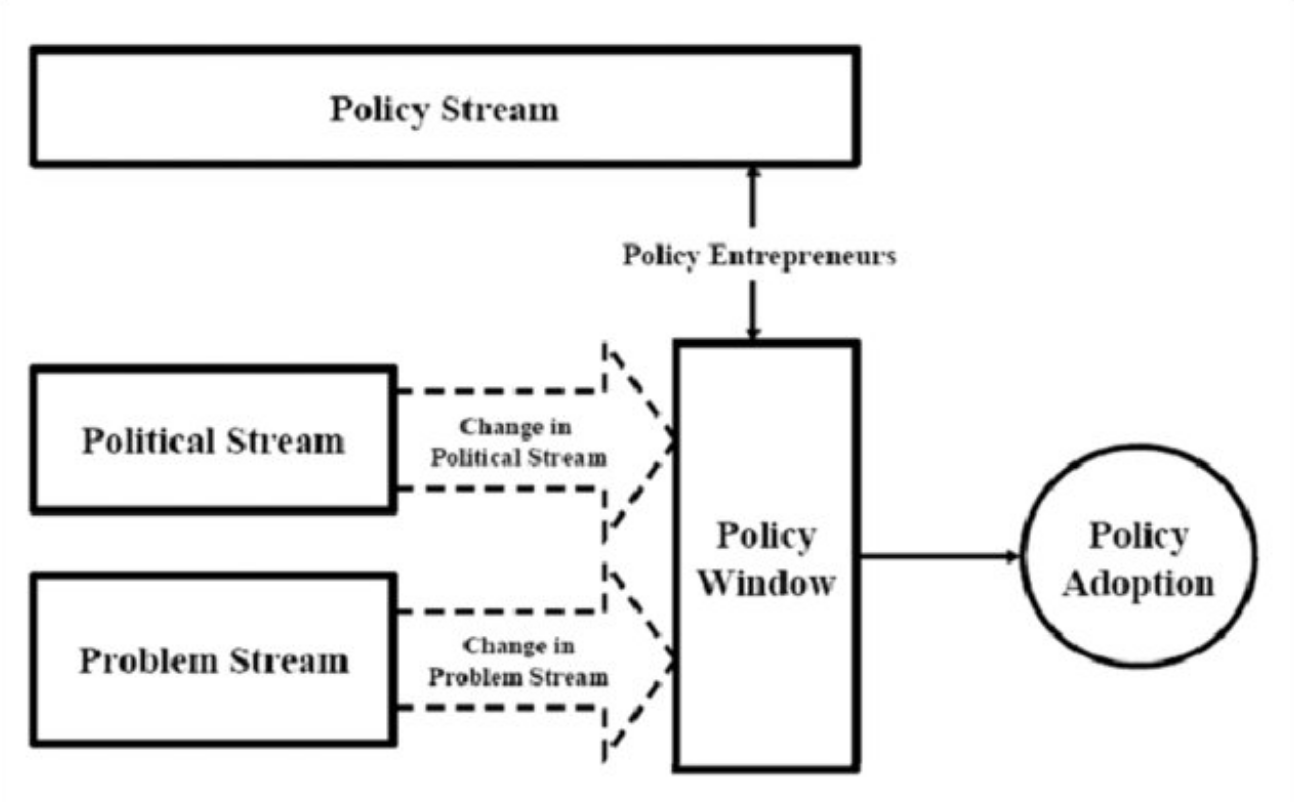
\includegraphics[scale=0.3]{windows.png}
     \end{center}
\end{column}
\end{columns}
\end{frame}

%@@@@@@@@@@@@@@@@@@@@@@@@@@@@@@@@@@@@@@@@@@@@@@@@@
\begin{frame}
\frametitle{Agenda Change}
\begin{columns}

\begin{column}{0.5\textwidth}

\begin{itemize}
\item Indicators = data that can be monitored for evidence of a worsening problem;
\bigskip
\bigskip
\item ``Problem streams" and ``political streams" may change rapidly due to a \textbf{focusing event}: a sudden event that can generate attention to public problems or issues, particularly issues and problems that are harmful;
\bigskip
\bigskip
\item The resulting pattern of policymaking is often called \textbf{punctuated equilibrium};
\end{itemize}
\end{column}
\begin{column}{0.5\textwidth}
    \begin{center}
     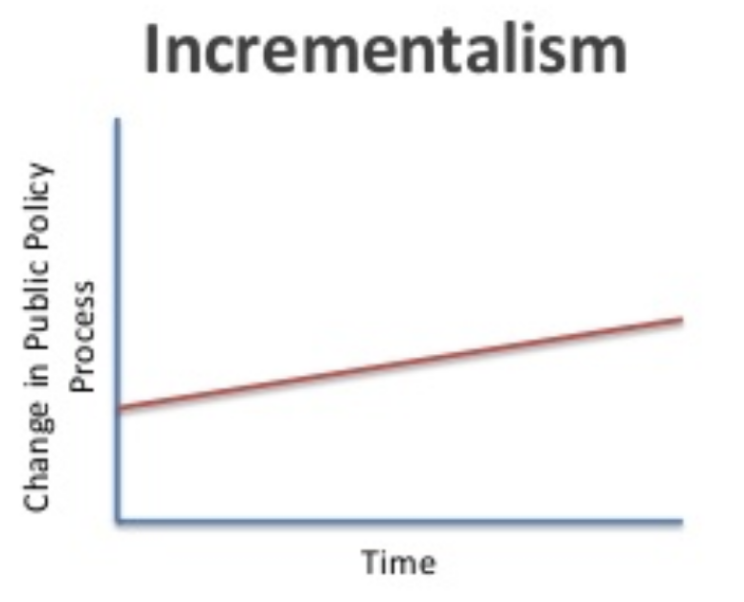
\includegraphics[scale=0.5]{incrementalism.png}
     \end{center}
\end{column}
\end{columns}
\end{frame}

%@@@@@@@@@@@@@@@@@@@@@@@@@@@@@@@@@@@@@@@@@@@@@@@@@
\begin{frame}
\frametitle{Agenda Change}
\begin{columns}

\begin{column}{0.5\textwidth}

\begin{itemize}
\item Indicators = data that can be monitored for evidence of a worsening problem;
\bigskip
\bigskip
\item ``Problem streams" and ``political streams" may change rapidly due to a \textbf{focusing event}: a sudden event that can generate attention to public problems or issues, particularly issues and problems that are harmful;
\bigskip
\bigskip
\item The resulting pattern of policymaking is often called \textbf{punctuated equilibrium};
\end{itemize}
\end{column}
\begin{column}{0.5\textwidth}
    \begin{center}
     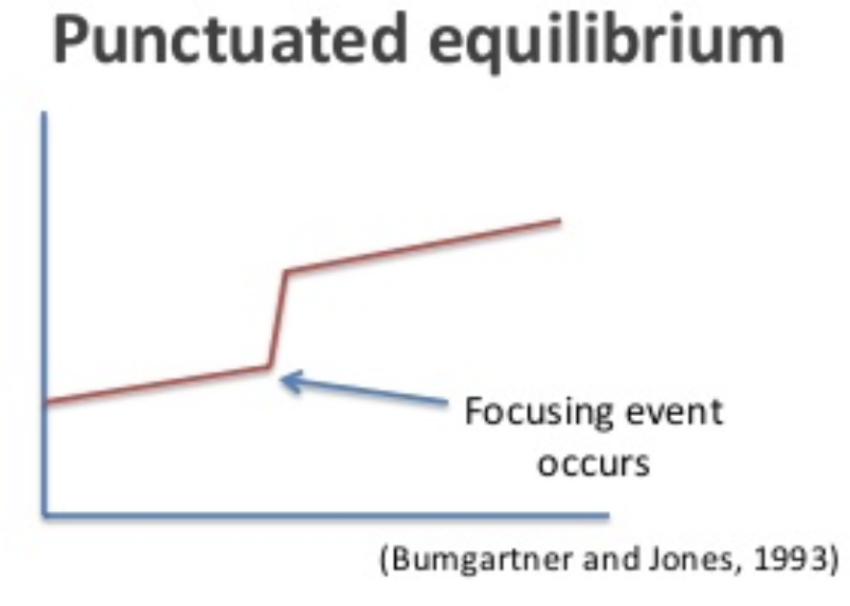
\includegraphics[scale=0.5]{punctuated_eq.png}
     \end{center}
\end{column}
\end{columns}
\end{frame}

%%@@@@@@@@@@@@@@@@@@@@@@@@@@@@@@@@@@@@@@@@@@@@@@@@@
%\begin{frame}
%\frametitle{Causality and Indicators}
%\begin{itemize}
%\item Tell a causal story (cause $\Rightarrow$ solution)!
%\bigskip
%\bigskip
%\item Use numbers to make the story more robust and `scientific';
%\bigskip
%\bigskip
%\item Deciding how to count is a policy decision (e.g. mean vs median);
%\end{itemize}
%\end{frame}

%@@@@@@@@@@@@@@@@@@@@@@@@@@@@@@@@@@@@@@@@@@@@@@@@@
\begin{frame}
\frametitle{Birkland$+$ Model of Policy}
\begin{itemize}
\item Policy Domain: what substantive problems are under consideration (e.g. water pollution, defense, etc.)???  This specifies:
\begin{itemize}
\item The actors involved, official actors who can make decisions $+$ stakeholders; 
\item Their organization, e.g. iron triangle, policy community;
\item the systemic agenda; 
\end{itemize}
\bigskip
\item \color{black}Input-output Model;
\begin{itemize}
\item Actors: legislature, executive, bureaucrats, justices and the available levers;
\item Inputs: agenda setting (application of power/social construction) specifies the institutional and decision agendas;
\item Black box decision making (structured by median voter thm, Arrow's thm) works on the decision agenda;
\item Outputs (e.g. statute laws, rules, court decisions);
\end{itemize}
\bigskip
\item Feedback and iteration.
\end{itemize}
\end{frame}

%@@@@@@@@@@@@@@@@@@@@@@@@@@@@@@@@@@@@@@@@@@@@@@@@@
\begin{frame}
\frametitle{Birkland$+$ Model of Policy}
\begin{itemize}
\item Policy Domain: what substantive problems are under consideration (e.g. water pollution, defense, etc.)???  This specifies:
\begin{itemize}
\item The actors involved, official actors who can make decisions $+$ stakeholders; 
\item Their organization, e.g. iron triangle, policy community;
\item the systemic agenda; 
\end{itemize}
\bigskip
\item \color{black}Input-output Model;
\begin{itemize}
\item Actors: legislature, executive, bureaucrats, justices and the available levers;
\item Inputs: agenda setting (application of power/social construction, \textbf{focusing events, indicator change}) specifies the institutional and decision agendas;
\item Black box decision making (structured by median voter thm, Arrow's thm) works on the decision agenda;
\begin{itemize}
\item \textbf{timing resembles incrementalism if driven by indicator change;}
\item \textbf{timing resembles punctuated equilibrium if driven by focusing events;}
 \end{itemize}
\item Outputs (e.g. statute laws, rules, court decisions);
\end{itemize}
\bigskip
\item Feedback and iteration.
\end{itemize}
\end{frame}

%@@@@@@@@@@@@@@@@@@@@@@@@@@@@@@@@@@@@@@@@@@@@@@@@@
\begin{frame}
\frametitle{Unofficial Actors}
\begin{center}
\Large \textbf{Participants in the process who do not have constitutionally or legally created incentives or mandates to be a part of the process, such as experts, researchers, and reporters, all of whom are important to the policy process.}
\end{center}
\end{frame}

%@@@@@@@@@@@@@@@@@@@@@@@@@@@@@@@@@@@@@@@@@@@@@@@@@
\begin{frame}
\frametitle{Unofficial Actors}
\begin{itemize}
\item Individual citizens;
\bigskip
\bigskip
\item Interest groups;
\bigskip
\bigskip
\item Political parties;
\bigskip
\bigskip
\item Think tanks;
\bigskip
\bigskip
\item Media.
\end{itemize}
\end{frame}

%@@@@@@@@@@@@@@@@@@@@@@@@@@@@@@@@@@@@@@@@@@@@@@@@@
\begin{frame}
\frametitle{Individual Citizens}
\begin{itemize}
\item Opportunities for individual participation are intermittent;
\begin{itemize}
\item Voting;
\item Letter writing;
\item Peaceful demonstrations (e.g. rallies, petitions, boycotts, etc.);
\end{itemize}
\bigskip
\item Participation in any of these is low with voting being highest (e.g. most elections have less than 50\% turnout);
\bigskip
\item How does government know what to do?
\end{itemize}
\end{frame}

%@@@@@@@@@@@@@@@@@@@@@@@@@@@@@@@@@@@@@@@@@@@@@@@@@
\begin{frame}
\frametitle{Individual Citizens}
    \begin{center}
     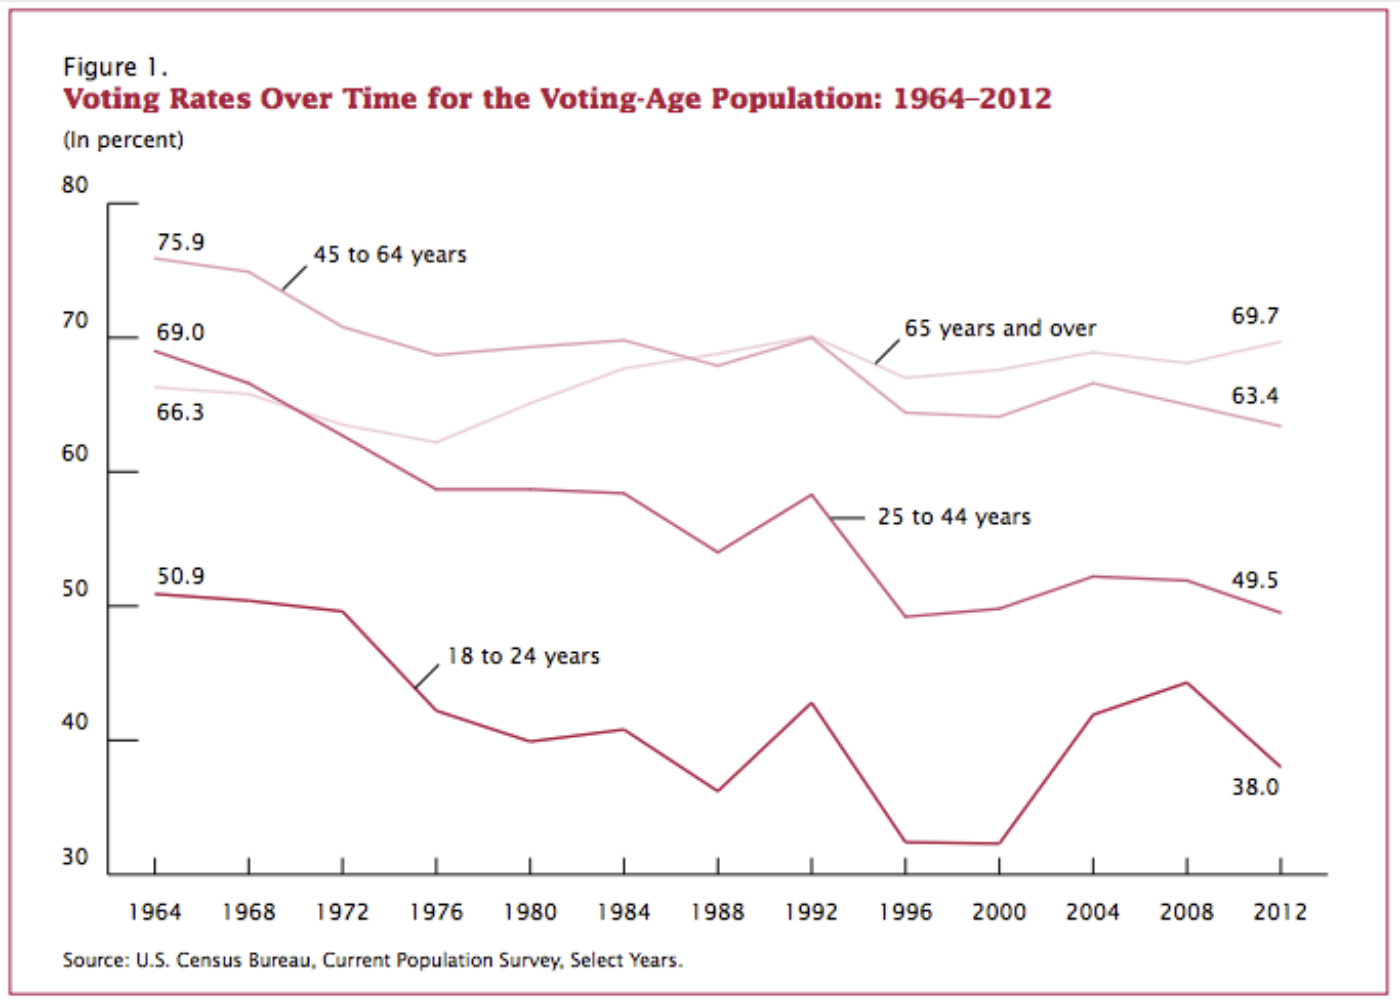
\includegraphics[scale=0.38]{Voting.png}
     \end{center}
\end{frame}

%@@@@@@@@@@@@@@@@@@@@@@@@@@@@@@@@@@@@@@@@@@@@@@@@@
\begin{frame}
\frametitle{Individual Citizens}
\begin{columns}

\begin{column}{0.5\textwidth}
\begin{itemize}
\item Ward 54 serves the Newell Smith Residence Hall;
\bigskip
\bigskip
\item Ward 56 serves Sellery Hall;
\bigskip
\bigskip
\item Ward 59 serves the Lakeshore Neighborhood.
\end{itemize}
\end{column}
\begin{column}{0.5\textwidth}  %%<--- here

    \begin{center}
     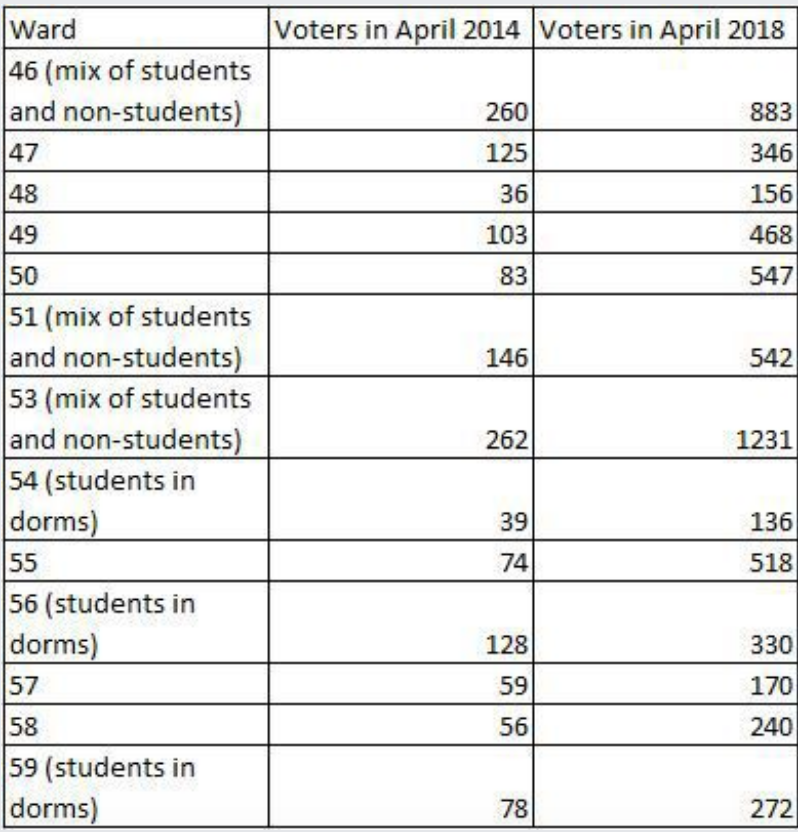
\includegraphics[scale=0.38]{UW_voting.png}
     \end{center}
     \end{column}
     \end{columns}
\end{frame}

%@@@@@@@@@@@@@@@@@@@@@@@@@@@@@@@@@@@@@@@@@@@@@@@@@
\begin{frame}
\frametitle{Interest groups}
\begin{center}
\Large A collection of people or organizations that unite to advance their desired political outcomes in government and society.
\end{center}
\end{frame}

%@@@@@@@@@@@@@@@@@@@@@@@@@@@@@@@@@@@@@@@@@@@@@@@@@
\begin{frame}
\frametitle{Interest groups}
\begin{itemize}
\item How do they form?
\begin{itemize}
\item Effective interest group formation is very expensive - tough to get people to join without benefits;
\item Mobilization around a high profile issue (e.g. civil rights, climate change);
\end{itemize}
\bigskip
\item Types of interest groups:
\begin{itemize}
\item Institutional - members belong to an institution (e.g. some unions);
\item Membership - members have chosen to join (e.g. Sierra Club, NRA);
\item Public - goal is to produce public goods, freeriding (e.g. Sierra Club);
\item Economic/private - benefits are for members (e.g. unions)
\end{itemize}
\bigskip
\item How do they policy-make?
\begin{itemize}
\item knowledge transfer (frame the problems);
\item communicating continuously with elected officials (i.e. lobbying -- do they buy votes?);
\item Protest;
\item Venue shopping.
\end{itemize}
\end{itemize}
\end{frame}

%@@@@@@@@@@@@@@@@@@@@@@@@@@@@@@@@@@@@@@@@@@@@@@@@@
\begin{frame}
\frametitle{Interest groups}
    \begin{center}
     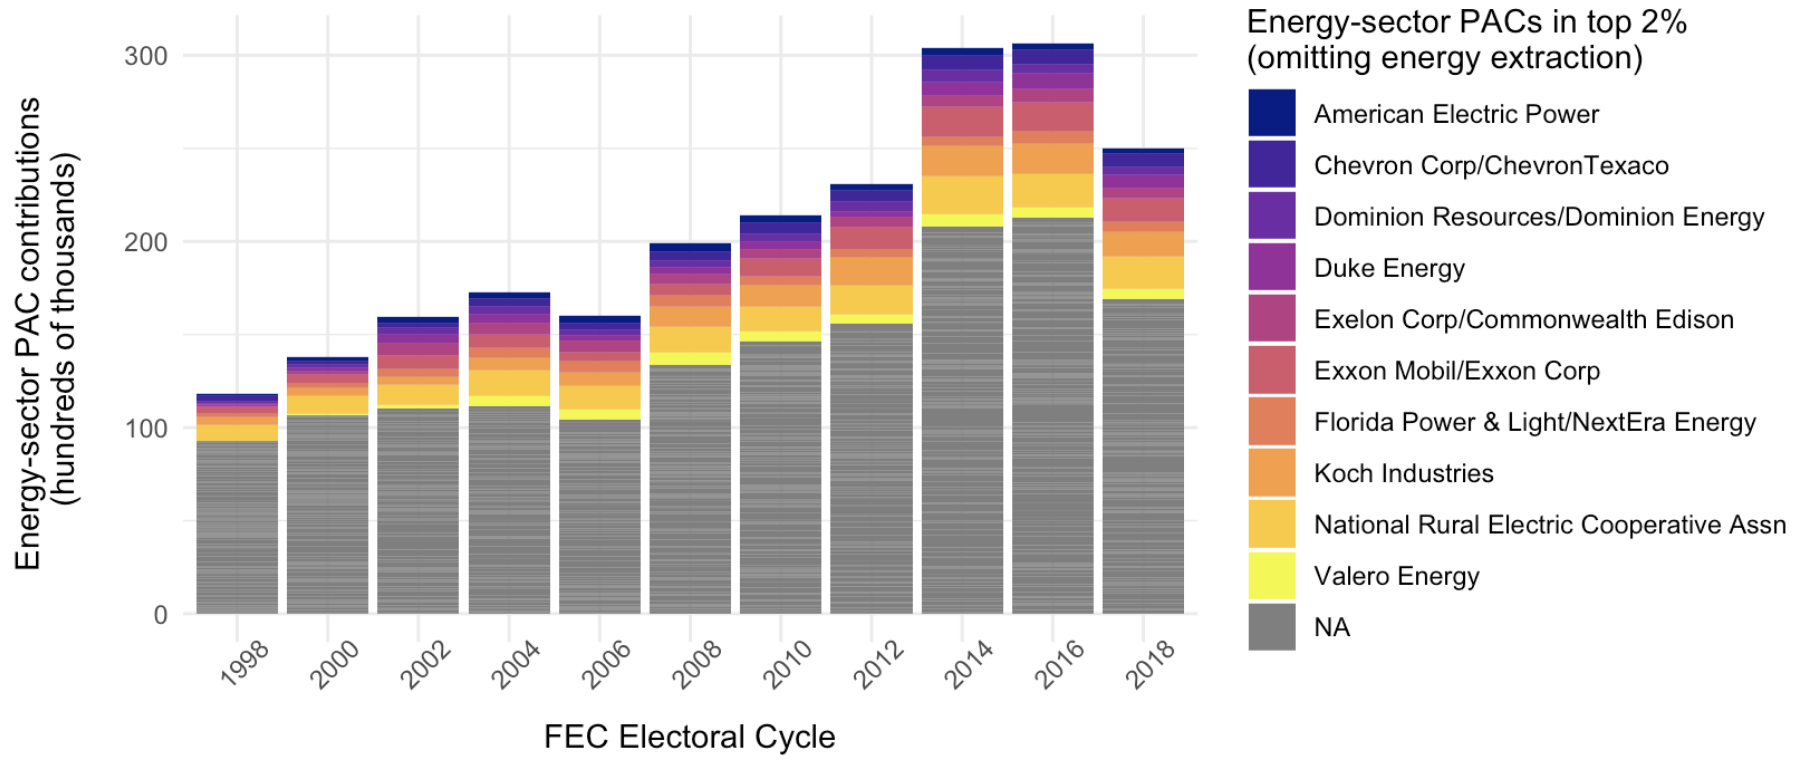
\includegraphics[scale=0.45]{Energy_PAC_Contributions.png}
     \end{center}
\end{frame}

%@@@@@@@@@@@@@@@@@@@@@@@@@@@@@@@@@@@@@@@@@@@@@@@@@
\begin{frame}
\frametitle{Interest groups}
Estimated Effect of Energy-Sector PAC Donations on Legislator Advocacy 
    \begin{center}
     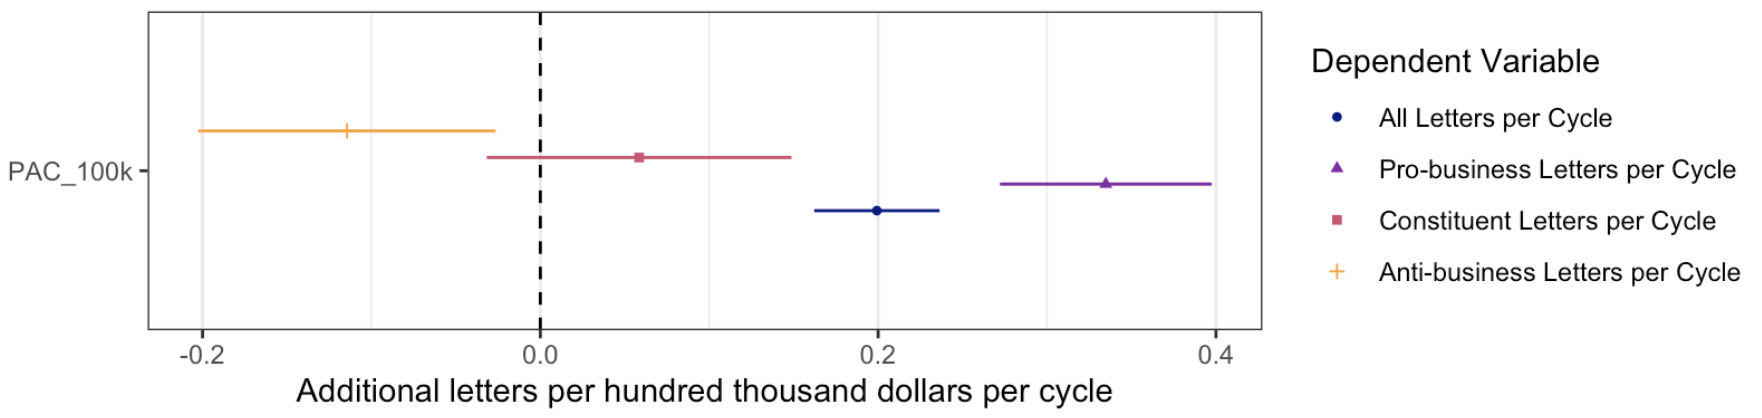
\includegraphics[scale=0.45]{Energy_PAC_effects.png}
     \end{center}
\end{frame}

%@@@@@@@@@@@@@@@@@@@@@@@@@@@@@@@@@@@@@@@@@@@@@@@@@
\begin{frame}
\frametitle{Interest groups}
Estimated Effect of Energy-Sector PAC Donations on Legislator Advocacy 
    \begin{center}
     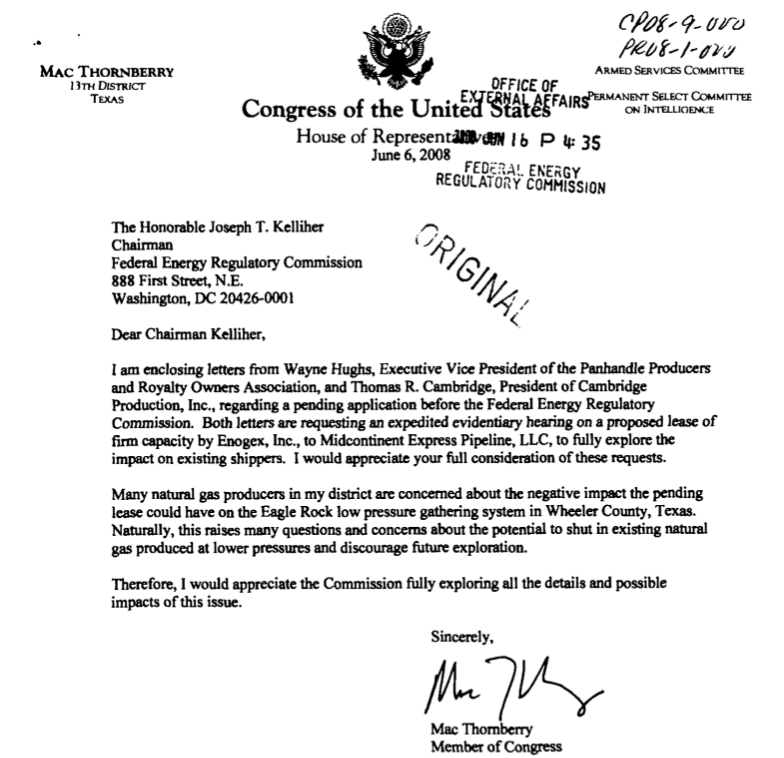
\includegraphics[scale=0.25]{FERC.png}
     \end{center}
\end{frame}

%@@@@@@@@@@@@@@@@@@@@@@@@@@@@@@@@@@@@@@@@@@@@@@@@@
\begin{frame}
\frametitle{Political parties}
\begin{itemize}
\item Provide labels to cue voters (wouldn't work without policy correlation);
\bigskip
\bigskip
\item Provide cues of electorate preferences;
\bigskip
\bigskip
\item Help elected officials create packages of policy ideas to appeal to voters and to shape legislation (e.g. contract with America);
\bigskip
\bigskip
\item Crucial to organization of Congress (e.g. election of Speaker, committee assignments).
\end{itemize}
\end{frame}

%@@@@@@@@@@@@@@@@@@@@@@@@@@@@@@@@@@@@@@@@@@@@@@@@@
\begin{frame}
\frametitle{Think tanks}
Information provision via research for a select audience (e.g. Brookings, Cato, RAND, etc.).
\end{frame}

%@@@@@@@@@@@@@@@@@@@@@@@@@@@@@@@@@@@@@@@@@@@@@@@@@
\begin{frame}
\frametitle{Media}
\begin{columns}

\begin{column}{0.5\textwidth}

``A popular Government, without popular information, or the means of acquiring it, is but a Prologue to a Farce or a Tragedy; or, perhaps both...And a people who mean to be their own Governors, must arm themselves with the power which knowledge gives." - James Madison (1822)\\
\bigskip

Information provision via research for a large audience (e.g. NYT, Washington Post, Chicago Tribune, etc.).
\end{column}
\begin{column}{0.5\textwidth}  %%<--- here
    \begin{center}
     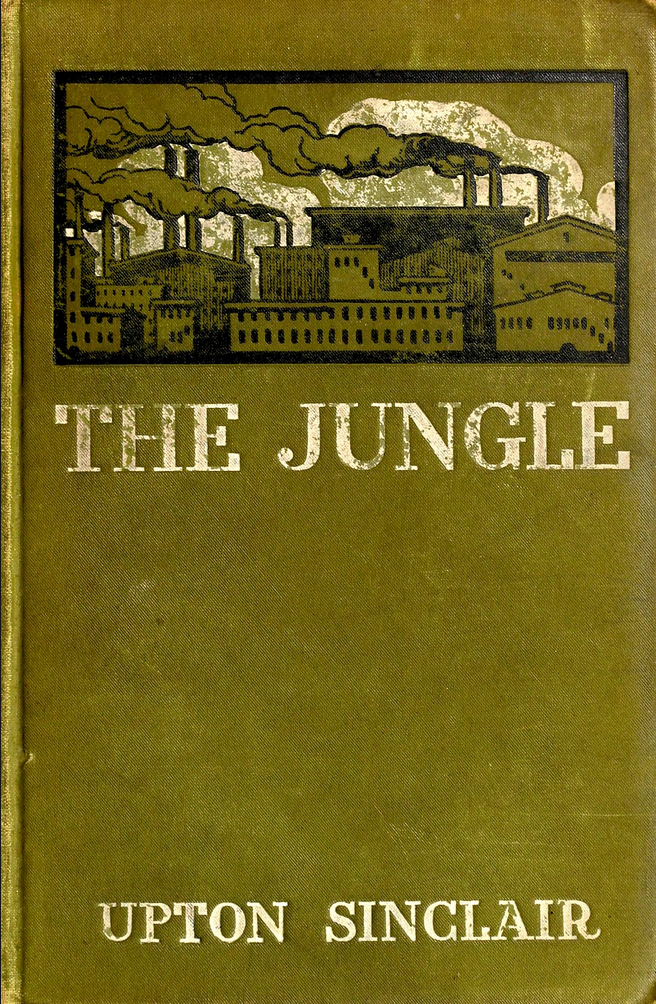
\includegraphics[scale=0.35]{jungle.png}
     \end{center}
\end{column}

\end{columns}

\end{frame}

%@@@@@@@@@@@@@@@@@@@@@@@@@@@@@@@@@@@@@@@@@@@@@@@@@
\begin{frame}
\frametitle{Media}
    \begin{center}
     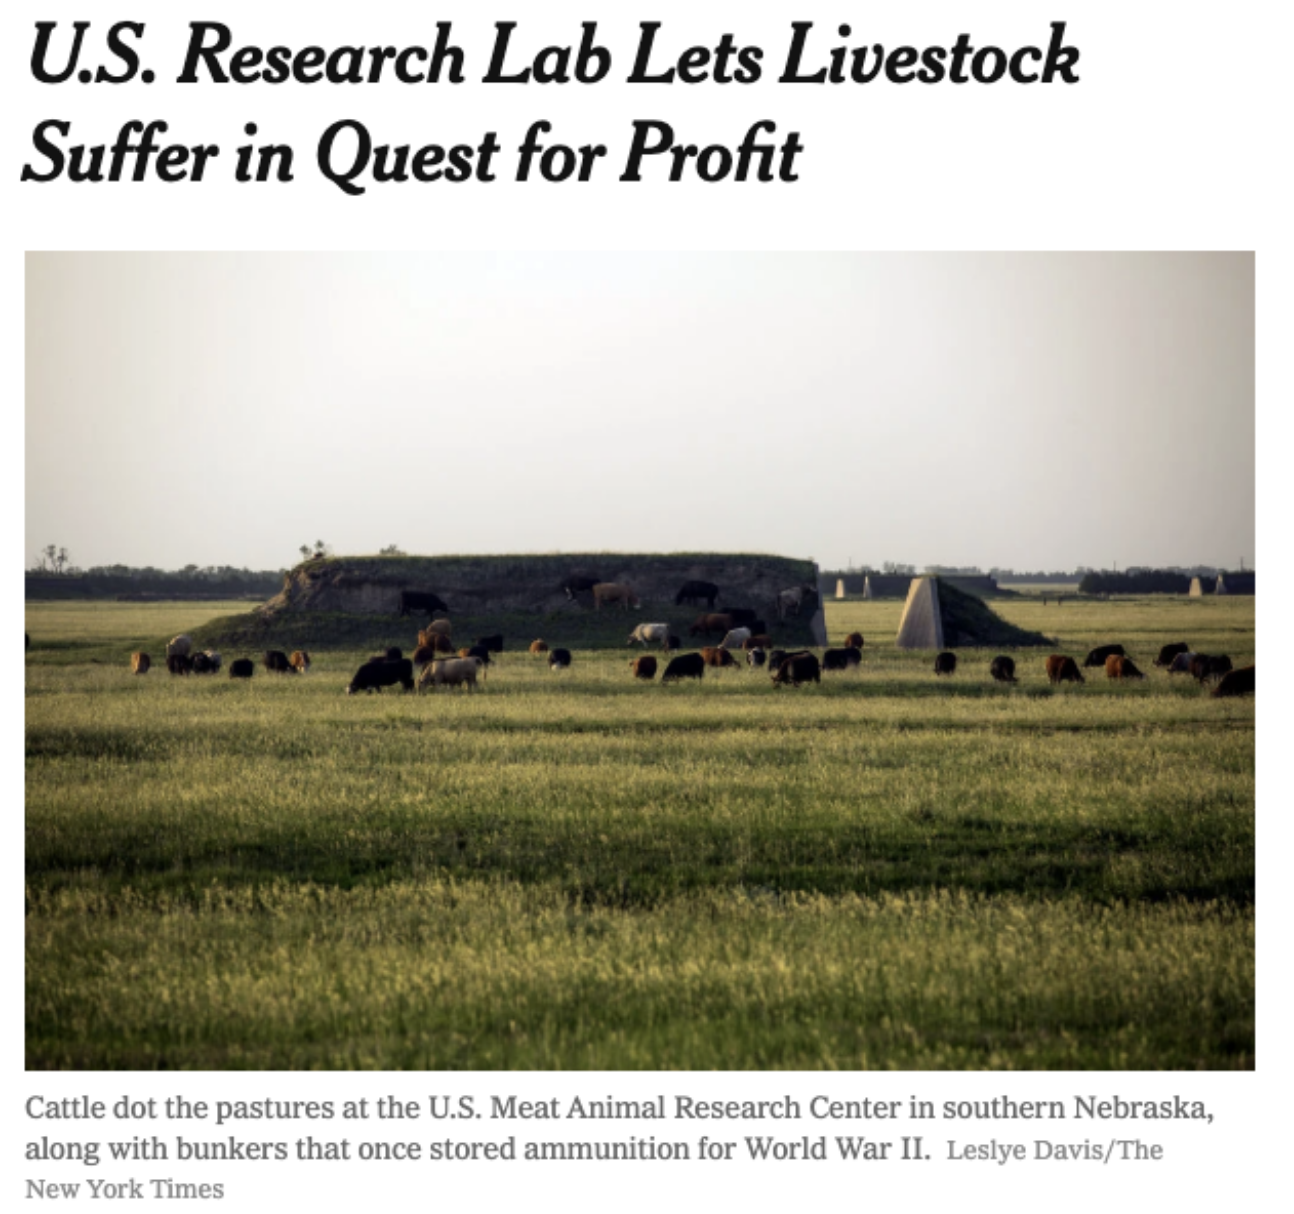
\includegraphics[scale=0.33]{media_example.png}
     \end{center}
\end{frame}

%@@@@@@@@@@@@@@@@@@@@@@@@@@@@@@@@@@@@@@@@@@@@@@@@@
\begin{frame}
\frametitle{Media}
    \begin{center}
     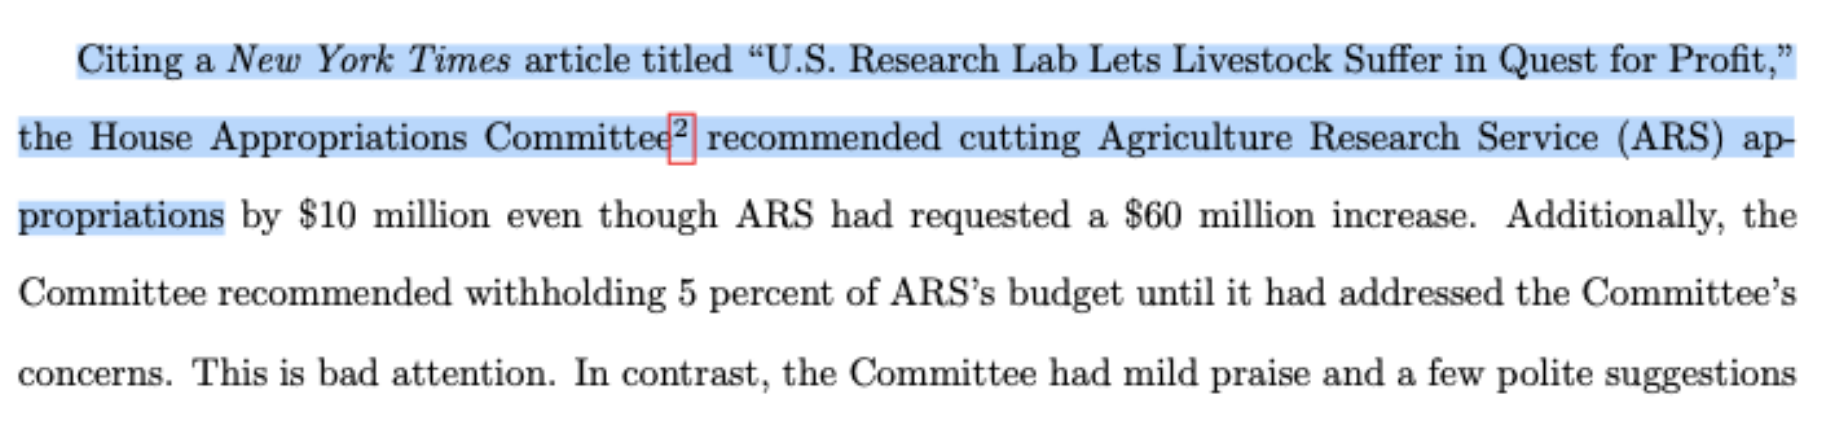
\includegraphics[scale=0.45]{media_consequences.png}
     \end{center}
\end{frame}

%@@@@@@@@@@@@@@@@@@@@@@@@@@@@@@@@@@@@@@@@@@@@@@@@@
\begin{frame}
\frametitle{Media}
    \begin{center}
     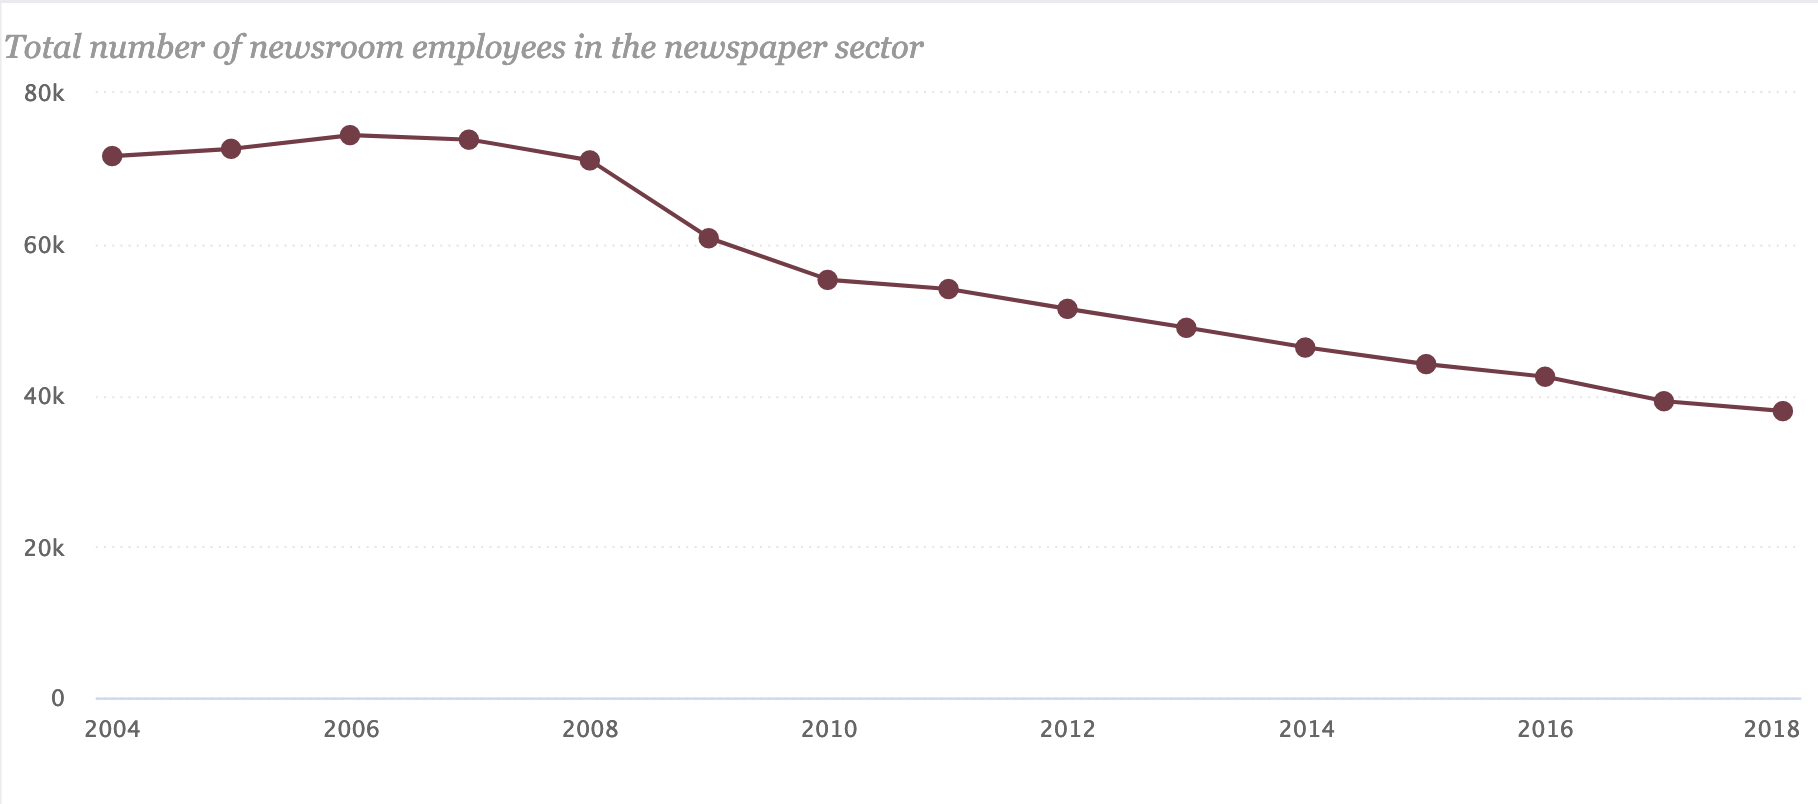
\includegraphics[scale=0.45]{newsrooms.png}
     \end{center}
\end{frame}

%@@@@@@@@@@@@@@@@@@@@@@@@@@@@@@@@@@@@@@@@@@@@@@@@@
\begin{frame}
\frametitle{Birkland$+$ Model of Policy}
\begin{itemize}
\item Policy Domain: what substantive problems are under consideration (e.g. water pollution, defense, etc.)???  This specifies:
\begin{itemize}
\item The actors involved, official actors who can make decisions $+$ stakeholders; 
\item Their organization, e.g. iron triangle, policy community;
\item the systemic agenda; 
\end{itemize}
\bigskip
\item \color{black}Input-output Model;
\begin{itemize}
\item Actors: legislature, executive, bureaucrats, justices and the available levers;
\item Inputs: agenda setting (application of power/social construction, focusing events, indicator change) specifies the institutional and decision agendas;
\item Black box decision making (structured by median voter thm, Arrow's thm) works on the decision agenda;
\begin{itemize}
\item timing resembles incrementalism if driven by indicator change;
\item timing resembles punctuated equilibrium if driven by focusing events;
 \end{itemize}
\item Outputs (e.g. statute laws, rules, court decisions);
\end{itemize}
\bigskip
\item Feedback and iteration.
\end{itemize}
\end{frame}

%@@@@@@@@@@@@@@@@@@@@@@@@@@@@@@@@@@@@@@@@@@@@@@@@@
\begin{frame}
\frametitle{Birkland$+$ Model of Policy}
\begin{itemize}
\item Policy Domain: what substantive problems are under consideration (e.g. water pollution, defense, etc.)???  This specifies:
\begin{itemize}
\item The actors involved, official actors who can make decisions $+$ stakeholders; 
\item Their organization, e.g. iron triangle, policy community;
\item the systemic agenda; 
\end{itemize} 
\bigskip
\item \color{black}Input-output Model;
\begin{itemize}
\item Actors: legislature, executive, bureaucrats, justices and the available levers;
\item Inputs: agenda setting (application of power/social construction, focusing events, indicator change \textbf{driven esp by unofficial actors}) specifies the institutional and decision agendas;
\item Black box decision making (structured by median voter thm, Arrow's thm) works on the decision agenda;
\begin{itemize}
\item timing resembles incrementalism if driven by indicator change;
\item timing resembles punctuated equilibrium if driven by focusing events;
 \end{itemize}
\item Outputs (e.g. statute laws, rules, court decisions);
\end{itemize}
\bigskip
\item Feedback and iteration.
\end{itemize}
\end{frame}

%@@@@@@@@@@@@@@@@@@@@@@@@@@@@@@@@@@@@@@@@@@@@@@@@@
\begin{frame}
\begin{center}
\Huge Policy Typologies
\end{center}
\end{frame}

%%@@@@@@@@@@@@@@@@@@@@@@@@@@@@@@@@@@@@@@@@@@@@@@@@@
%\begin{frame}
%\frametitle{Policy}
%\begin{center}
%\Large A statement by government of what it intends to do or not to do...
%\end{center}
%\end{frame}

%@@@@@@@@@@@@@@@@@@@@@@@@@@@@@@@@@@@@@@@@@@@@@@@@@
\begin{frame}
\frametitle{Typology}
\begin{center}
\Large A system for categorizing things based on similar characteristics, and for differentiating things with different characteristics.
\end{center}
\end{frame}

%%@@@@@@@@@@@@@@@@@@@@@@@@@@@@@@@@@@@@@@@@@@@@@@@@@
%\begin{frame}
%\frametitle{Typology 1: Levels of Policy Codification}
%\begin{itemize}
%\item Constitutional -- constitutions, highly visible;
%\bigskip
%\item Statutory -- US code, highly visible;
%\bigskip
%\item Regulatory -- Federal register, moderately visible;
%\bigskip
%\item Formal SOPs -- Operating procedures, low visibility;
%\bigskip
%\item Patterned behavior -- Not formally codified, low visibility;
%\bigskip
%\item Subtle changes in cognition/problem definition -- seen in revealed behavior, very low visibility.
%\end{itemize}
%\end{frame}
%
%%@@@@@@@@@@@@@@@@@@@@@@@@@@@@@@@@@@@@@@@@@@@@@@@@@
%\begin{frame}
%\frametitle{Typology 2 (Lowi)}
%\begin{itemize}
%\item Distributive -- e.g. park barrel spending, congressional committees/executive agencies, logrolling, low visibility;
%\bigskip
%\bigskip
%\item Protective regulatory -- e.g. CWA, congressional committees/executive agencies/trade associations, bargaining, moderate;
%\bigskip
%\bigskip
%\item Competitive regulatory -- e.g. utilities, FCC, congressional committees/executive agencies/interest groups, logrolling, low visibility;
%\bigskip
%\bigskip
%\item Redistributive -- highly controversial, president/congress as a whole, ideological conflict, high visibility.
%\end{itemize}
%\end{frame}

%@@@@@@@@@@@@@@@@@@@@@@@@@@@@@@@@@@@@@@@@@@@@@@@@@
\begin{frame}
\frametitle{Typology 3 (Wilson)}
\begin{itemize}
\item Concentrated costs, distributed benefits -- entreprenurial groups persuade policy makers to regulate in the public interest, opposition from costed groups;
\bigskip
\bigskip
\item Concentrated costs, concentrated benefits -- interest groups play a zero sum game;
\bigskip
\bigskip
\item Distributed costs, distributed benefits -- majoritarian politics, often leads to weak, ambiguous policies;
\bigskip
\bigskip
\item Distributed costs, concentrated benefits -- close ``clientele" relationships between policy makers, regulators, and the regulated interest.
\end{itemize}
\end{frame}

%@@@@@@@@@@@@@@@@@@@@@@@@@@@@@@@@@@@@@@@@@@@@@@@@@
\begin{frame}
\begin{center}
\Huge Why should you care???\\
\bigskip
\bigskip
\onslide<2->
\Large Because knowing what \textbf{type} of policy you are dealing with allows you to predict how much conflict you will face.
\end{center}
\end{frame}

%@@@@@@@@@@@@@@@@@@@@@@@@@@@@@@@@@@@@@@@@@@@@@@@@@
\begin{frame}
\frametitle{Birkland$+$ Model of Policy}
\begin{itemize}
\item Policy Domain: what substantive problems are under consideration (e.g. water pollution, defense, etc.)???  This specifies:
\begin{itemize}
\item The actors involved, official actors who can make decisions $+$ stakeholders; 
\item Their organization, e.g. iron triangle, policy community;
\item the systemic agenda; 
\end{itemize}
\bigskip
\item \color{black}Input-output Model;
\begin{itemize}
\item Actors: legislature, executive, bureaucrats, justices and the available levers;
\item Inputs: agenda setting (application of power/social construction, focusing events, indicator change driven esp by unofficial actors) specifies the institutional and decision agendas;
\item Black box decision making (structured by median voter thm, Arrow's thm) works on the decision agenda;
\begin{itemize}
\item timing resembles incrementalism if driven by indicator change;
\item timing resembles punctuated equilibrium if driven by focusing events;
 \end{itemize}
\item Outputs (e.g. statute laws, rules, court decisions);
\end{itemize}
\bigskip
\item Feedback and iteration.
\end{itemize}
\end{frame}

%@@@@@@@@@@@@@@@@@@@@@@@@@@@@@@@@@@@@@@@@@@@@@@@@@
\begin{frame}
\frametitle{Birkland$+$ Model of Policy}
\begin{itemize}
\item Policy Domain: what substantive problems are under consideration (e.g. water pollution, defense, etc.)???  This specifies:
\begin{itemize}
\item The actors involved, official actors who can make decisions $+$ stakeholders; 
\item \textbf{Distribution of benefits/costs} $\Rightarrow$ actor organization, e.g. iron triangle, policy community;
\item The systemic agenda; 
\end{itemize} 
\bigskip
\item \color{black}Input-output Model;
\begin{itemize}
\item Actors: legislature, executive, bureaucrats, justices and the available levers;
\item Inputs: agenda setting (application of power/social construction, focusing events, indicator change driven esp by unofficial actors) specifies the institutional and decision agendas;
\item Black box decision making (structured by median voter thm, Arrow's thm) works on the decision agenda;
\begin{itemize}
\item timing resembles incrementalism if driven by indicator change;
\item timing resembles punctuated equilibrium if driven by focusing events;
 \end{itemize}
\item Outputs (e.g. statute laws, rules, court decisions);
\end{itemize}
\bigskip
\item Feedback and iteration.
\end{itemize}
\end{frame}

%@@@@@@@@@@@@@@@@@@@@@@@@@@@@@@@@@@@@@@@@@@@@@@@@@
\begin{frame}
\frametitle{Preparing to design policies}
\begin{itemize}
\item What does success look like?
\begin{itemize}
\item \textbf{Outputs}: \color{white}formal laws, regulations, rules, etc. -- these are easy to understand and track and have clear implications, e.g. resourcing requirements;\color{black}
\item \textbf{Outcomes}: \color{white}the realized substantive impact of an implemented policy -- these are potentially hard to measure and are relative to the problem definition;
\item[] Agencies tend to measure outputs b/c it's easy!\color{black}
\end{itemize}
\bigskip
\item Five steps of policy design to consider:
\begin{enumerate}
\item Goals;
\item Causal Model;
\item Policy Tools;
\item Decisions;
\item Implementation.
\end{enumerate}
\end{itemize}
\end{frame}

%@@@@@@@@@@@@@@@@@@@@@@@@@@@@@@@@@@@@@@@@@@@@@@@@@
\begin{frame}
\frametitle{Preparing to design policies}
\begin{itemize}
\item What does success look like?
\begin{itemize}
\item \textbf{Outputs}: formal laws, regulations, rules, etc. -- these are easy to understand and track and have clear implications, e.g. resourcing requirements;
\item \textbf{Outcomes}: \color{white}the realized substantive impact of an implemented policy -- these are potentially hard to measure and are relative to the problem definition;
\item[] Agencies tend to measure outputs b/c it's easy!\color{black}
\end{itemize}
\bigskip
\item Five steps of policy design to consider:
\begin{enumerate}
\item Goals;
\item Causal Model;
\item Policy Tools;
\item Decisions;
\item Implementation.
\end{enumerate}
\end{itemize}
\end{frame}

%@@@@@@@@@@@@@@@@@@@@@@@@@@@@@@@@@@@@@@@@@@@@@@@@@
\begin{frame}
\frametitle{Preparing to design policies}
\begin{itemize}
\item What does success look like?
\begin{itemize}
\item \textbf{Outputs}: formal laws, regulations, rules, etc. -- these are easy to understand and track and have clear implications, e.g. resourcing requirements;
\item \textbf{Outcomes}: the realized substantive impact of an implemented policy -- these are potentially hard to measure and are relative to the problem definition;
\item Agencies tend to measure outputs b/c it's easy!
\end{itemize}
\bigskip
\item Five steps of policy design to consider:
\begin{enumerate}
\item Goals;
\item Causal Model;
\item Policy Tools;
\item Decisions;
\item Implementation.
\end{enumerate}
\end{itemize}
\end{frame}

%@@@@@@@@@@@@@@@@@@@@@@@@@@@@@@@@@@@@@@@@@@@@@@@@@
\begin{frame}
\frametitle{Birkland$+$ Model of Policy}
\begin{itemize}
\item Policy Domain: what substantive problems are under consideration (e.g. water pollution, defense, etc.)???  This specifies:
\begin{itemize}
\item The actors involved, official actors who can make decisions $+$ stakeholders; 
\item Distribution of benefits/costs $\Rightarrow$ actor organization, e.g. iron triangle, policy community;
\item The systemic agenda; 
\end{itemize} 
\bigskip
\item \color{black}Input-output Model;
\begin{itemize}
\item Actors: legislature, executive, bureaucrats, justices and the available levers;
\item Inputs: agenda setting (application of power/social construction, focusing events, indicator change driven esp by unofficial actors) specifies the institutional and decision agendas;
\item Black box decision making (structured by median voter thm, Arrow's thm) works on the decision agenda;
\begin{itemize}
\item timing resembles incrementalism if driven by indicator change;
\item timing resembles punctuated equilibrium if driven by focusing events;
 \end{itemize}
\item Outputs (e.g. statute laws, rules, court decisions);
\end{itemize}
\bigskip
\item Feedback and iteration.
\end{itemize}
\end{frame}

%@@@@@@@@@@@@@@@@@@@@@@@@@@@@@@@@@@@@@@@@@@@@@@@@@
\begin{frame}
\frametitle{Birkland$+$ Model of Policy}
\begin{itemize}
\item Policy Domain: what substantive problems are under consideration (e.g. water pollution, defense, etc.)???  This specifies:
\begin{itemize}
\item The actors involved, official actors who can make decisions $+$ stakeholders; 
\item Distribution of benefits/costs $\Rightarrow$ actor organization, e.g. iron triangle, policy community;
\item The systemic agenda; 
\end{itemize}
\bigskip
\item \color{black}Input-output Model;
\begin{itemize}
\item Actors: legislature, executive, bureaucrats, justices and the available levers;
\item Inputs: agenda setting (application of power/social construction, focusing events, indicator change driven esp by unofficial actors) specifies the institutional and decision agendas;
\item Black box decision making (structured by median voter thm, Arrow's thm) works on the decision agenda;
\begin{itemize}
\item timing resembles incrementalism if driven by indicator change;
\item timing resembles punctuated equilibrium if driven by focusing events;
 \end{itemize}
\item \textbf{Outputs} (e.g. statute laws, rules, court decisions);
\end{itemize}
\bigskip
\item \textbf{Outcomes}: Feedback and iteration.
\end{itemize}
\end{frame}

%@@@@@@@@@@@@@@@@@@@@@@@@@@@@@@@@@@@@@@@@@@@@@@@@@
\begin{frame}
\frametitle{Step 1: Define Goals}
\begin{itemize}
\item Policy is made to solve a problem -- this implies a \textbf{goal};
\bigskip
\item Many different, potentially conflicting goals possible:
\begin{itemize}
\item \textbf{Equity}\color{white} - how to divide resources;\color{black}
\item \textbf{Efficiency}\color{white} - maximizing output given inputs;\color{black}
\item \textbf{Security}\color{white} - ensuring we stay out of the state of nature;\color{black}
\item \textbf{Liberty}\color{white} - maximizing our ability to make unconstrained choices;\color{black}
\end{itemize}
\bigskip
\item Optimal policy depends on how these goals are weighted against each other;
\bigskip
\item Goal conflict: some of our most contentious policies are problematic because different people have different weights;
\bigskip
\item Example: \color{white}both gun control and abortion policy involve both liberty and security.
\end{itemize}
\end{frame}

%@@@@@@@@@@@@@@@@@@@@@@@@@@@@@@@@@@@@@@@@@@@@@@@@@
\begin{frame}
\frametitle{Step 1: Define Goals}
\begin{itemize}
\item Policy is made to solve a problem -- this implies a \textbf{goal};
\bigskip
\item Many different, potentially conflicting goals possible:
\begin{itemize}
\item \textbf{Equity} - how to divide resources;
\item \textbf{Efficiency} - maximizing output given inputs;
\item \textbf{Security} - ensuring we stay out of the state of nature;
\item \textbf{Liberty} - maximizing our ability to make unconstrained choices;
\end{itemize}
\bigskip
\item Optimal policy depends on how these goals are weighted against each other;
\bigskip
\item Goal conflict: some of our most contentious policies are problematic because different people have different weights;
\bigskip
\item Example: \color{white}both gun control and abortion policy involve both liberty and security.
\end{itemize}
\end{frame}

%@@@@@@@@@@@@@@@@@@@@@@@@@@@@@@@@@@@@@@@@@@@@@@@@@
\begin{frame}
\frametitle{Step 1: Define Goals}
\begin{itemize}
\item Policy is made to solve a problem -- this implies a \textbf{goal};
\bigskip
\item Many different, potentially conflicting goals possible:
\begin{itemize}
\item \textbf{Equity} - how to divide resources;
\item \textbf{Efficiency} - maximizing output given inputs;
\item \textbf{Security} - ensuring we stay out of the state of nature;
\item \textbf{Liberty} - maximizing our ability to make unconstrained choices;
\end{itemize}
\bigskip
\item Optimal policy depends on how these goals are weighted against each other;
\bigskip
\item Goal conflict: some of our most contentious policies are problematic because different people have different weights;
\bigskip
\item Example: both gun control and abortion policy involve both liberty and security.
\end{itemize}
\end{frame}

%@@@@@@@@@@@@@@@@@@@@@@@@@@@@@@@@@@@@@@@@@@@@@@@@@
\begin{frame}
\frametitle{Step 2: Set up a causal theory}
\begin{columns}
\begin{column}{0.5\textwidth}

\begin{itemize}
\item What \textbf{causes} the problem we want to solve?
\bigskip
\bigskip
\item Very complicated - entire scientific disciplines are devoted to answering these questions;
\bigskip
\bigskip
\item Most basic question: is a problem due to an act of God or to something that has pullable levers (implies liability)?
\end{itemize}

\end{column}
\begin{column}{0.5\textwidth}  %%<--- here

    \begin{center}
     \includegraphics[scale=0.35]{climate.png}
     \end{center}
     \end{column}
     \end{columns}

\end{frame}

%@@@@@@@@@@@@@@@@@@@@@@@@@@@@@@@@@@@@@@@@@@@@@@@@@
\begin{frame}
\frametitle{Birkland$+$ Model of Policy}
\begin{itemize}
\item Policy Domain: what substantive problems are under consideration (e.g. water pollution, defense, etc.)???  This specifies:
\begin{itemize}
\item The actors involved, official actors who can make decisions $+$ stakeholders; 
\item Distribution of benefits/costs $\Rightarrow$ actor organization, e.g. iron triangle, policy community;
\item The systemic agenda; 
\end{itemize}
\bigskip
\item \color{black}Input-output Model;
\begin{itemize}
\item Actors: legislature, executive, bureaucrats, justices and the available levers;
\item Inputs: agenda setting (application of power/social construction, focusing events, indicator change driven esp by unofficial actors) specifies the institutional and decision agendas;
\item Black box decision making (structured by median voter thm, Arrow's thm) works on the decision agenda;
\begin{itemize}
\item timing resembles incrementalism if driven by indicator change;
\item timing resembles punctuated equilibrium if driven by focusing events;
 \end{itemize}
\item \textbf{Outputs} (e.g. statute laws, rules, court decisions);
\end{itemize}
\bigskip
\item \textbf{Outcomes}: Feedback and iteration.
\end{itemize}
\end{frame}

%@@@@@@@@@@@@@@@@@@@@@@@@@@@@@@@@@@@@@@@@@@@@@@@@@
\begin{frame}
\frametitle{Birkland$+$ Model of Policy}
\begin{itemize}
\item Policy Domain: what substantive problems are under consideration (e.g. water pollution, defense, etc.)???  This specifies:
\begin{itemize}
\item The actors involved, official actors who can make decisions $+$ stakeholders; 
\item Distribution of benefits/costs $\Rightarrow$ actor organization, e.g. iron triangle, policy community;
\item The systemic agenda; 
\end{itemize}
\bigskip
\item \color{black}Input-output Model;
\begin{itemize}
\item Actors: legislature, executive, bureaucrats, justices and the available levers;
\item Inputs: agenda setting (application of power/social construction, focusing events, indicator change driven esp by unofficial actors) \textbf{sets goals, determines the causal model}, and specifies the institutional and decision agendas;
\item Black box decision making (structured by median voter thm, Arrow's thm) works on the decision agenda;
\begin{itemize}
\item timing resembles incrementalism if driven by indicator change;
\item timing resembles punctuated equilibrium if driven by focusing events;
 \end{itemize}
\item \textbf{Outputs} (e.g. statute laws, rules, court decisions);
\end{itemize}
\bigskip
\item \textbf{Outcomes}: Feedback and iteration.
\end{itemize}
\end{frame}

%@@@@@@@@@@@@@@@@@@@@@@@@@@@@@@@@@@@@@@@@@@@@@@@@@
\begin{frame}
\frametitle{Step 3: Formulate Policy Tools}
\begin{itemize}
\item Four dimensions:
\begin{enumerate}
\item What is the activity government is doing (See Bardach!);
\item What is the structure of the delivery system (direct like social security, or indirect like block grants?);
\item How centralized (defense or forestry?);
\item Automatic or administrated (tax incentives are self-executing vs welfare systems which require adjudication);
\end{enumerate}
\bigskip
\bigskip

\item Can also think about coercive vs non-coercive policy tools as it applies to target behavior.
\end{itemize}
\end{frame}

%@@@@@@@@@@@@@@@@@@@@@@@@@@@@@@@@@@@@@@@@@@@@@@@@@
\begin{frame}
\frametitle{Birkland$+$ Model of Policy}
\begin{itemize}
\item Policy Domain: what substantive problems are under consideration (e.g. water pollution, defense, etc.)???  This specifies:
\begin{itemize}
\item The actors involved, official actors who can make decisions $+$ stakeholders; 
\item Distribution of benefits/costs $\Rightarrow$ actor organization, e.g. iron triangle, policy community;
\item The systemic agenda; 
\end{itemize}
\bigskip
\item \color{black}Input-output Model;
\begin{itemize}
\item Actors: legislature, executive, bureaucrats, justices and the available levers;
\item Inputs: agenda setting (application of power/social construction, focusing events, indicator change driven esp by unofficial actors) sets goals, determines the causal model, and specifies the institutional and decision agendas;
\item Black box decision making (structured by median voter thm, Arrow's thm) works on the decision agenda;
\begin{itemize}
\item timing resembles incrementalism if driven by indicator change;
\item timing resembles punctuated equilibrium if driven by focusing events;
 \end{itemize}
\item \textbf{Outputs} (e.g. statute laws, rules, court decisions);
\end{itemize}
\bigskip
\item \textbf{Outcomes}: Feedback and iteration.
\end{itemize}
\end{frame}

%@@@@@@@@@@@@@@@@@@@@@@@@@@@@@@@@@@@@@@@@@@@@@@@@@
\begin{frame}
\frametitle{Birkland$+$ Model of Policy}
\begin{itemize}
\item Policy Domain: what substantive problems are under consideration (e.g. water pollution, defense, etc.)???  This specifies:
\begin{itemize}
\item The actors involved, official actors who can make decisions $+$ stakeholders; 
\item Distribution of benefits/costs $\Rightarrow$ actor organization, e.g. iron triangle, policy community;
\item The systemic agenda; 
\end{itemize}
\bigskip
\item \color{black}Input-output Model;
\begin{itemize}
\item Actors: legislature, executive, bureaucrats, justices and the available levers;
\item Inputs: agenda setting (application of power/social construction, focusing events, indicator change driven esp by unofficial actors) sets goals, determines the causal model, \textbf{which specifies the institutional agenda, and leads to the policies on the decision agenda;}
\item Black box decision making (structured by median voter thm, Arrow's thm) works on the decision agenda;
\begin{itemize}
\item timing resembles incrementalism if driven by indicator change;
\item timing resembles punctuated equilibrium if driven by focusing events;
 \end{itemize}
\item \textbf{Outputs} (e.g. statute laws, rules, court decisions);
\end{itemize}
\bigskip
\item \textbf{Outcomes}: Feedback and iteration.
\end{itemize}
\end{frame}

%@@@@@@@@@@@@@@@@@@@@@@@@@@@@@@@@@@@@@@@@@@@@@@@@@
\begin{frame}
\frametitle{Step 4: Policy makers decide -- but how?}
\begin{itemize}
\item These are going to be \textbf{models} -- they can be \textbf{Positive} vs \textbf{Normative};
\item Imagine that a policy has reached the \textbf{decision agenda}:
\item Rational Choice:
\begin{itemize}
\item Decision makers confront a problem; gather information; analyze options; choose that which maximizes gain;
\item Advantages: extremely powerful; extensive theoretical interdisciplinary literature;
\item Critiques: goal conflict; large info processing reqs; 
\end{itemize}
\item Bounded Rationality:
\begin{itemize}
\item Do rational choice with constraints on time, info, and cognitive ability;
\item Critiques: undisciplined;
\end{itemize}
\item Incrementalism:
\begin{itemize}
\item Policy change in incremental steps that allow decision makers to adjust policies as they learn from their successes and failures;
\item Critiques: empirically, some problems have had bold solutions (e.g. mobilization for WWII, race to the moon); 
\end{itemize}
\end{itemize}
\end{frame}

%@@@@@@@@@@@@@@@@@@@@@@@@@@@@@@@@@@@@@@@@@@@@@@@@@
\begin{frame}
\frametitle{Step 5: Implementation}
\begin{columns}
\begin{column}{0.5\textwidth}

\begin{itemize}
\item So, your bill has become a law... what next?!
\bigskip
\bigskip
\bigskip
\item \textbf{Implementation}: the process by which policies \textbf{enacted} by government are \textbf{put into effect} by the relevant \textbf{agencies};
\bigskip
\bigskip
\bigskip
\item May involve delegation and bargaining!
\end{itemize}

\end{column}
\begin{column}{0.5\textwidth}
    \begin{center}
     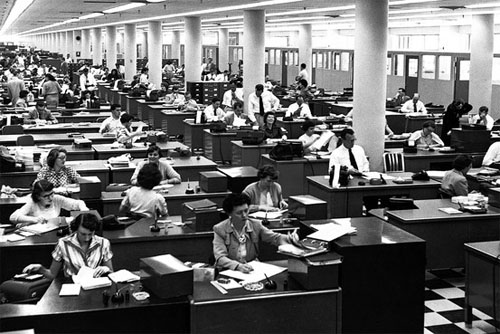
\includegraphics[scale=0.4]{bureaucracy1.jpeg}
     \end{center}

\end{column}
\end{columns}

\end{frame}

%@@@@@@@@@@@@@@@@@@@@@@@@@@@@@@@@@@@@@@@@@@@@@@@@@
\begin{frame}
\frametitle{How do we study implementation?}

\begin{itemize}
\item Before 1970s, via thick description -- detailed case studies of individual policy topics;
\bigskip
\bigskip
\item After 1970s, build systematic theories meant to explain many case studies:
\begin{itemize}
\item Top down implementation;
\item Bottom up implementation;
\end{itemize}
\bigskip
\bigskip
\item Finally, synthesis -- a unified model of policy implementation.
\end{itemize}

\end{frame}

%@@@@@@@@@@@@@@@@@@@@@@@@@@@@@@@@@@@@@@@@@@@@@@@@@
\begin{frame}
\frametitle{Top down implementation}

\begin{itemize}
\item Hierarchical; begins with goals of top level of policy-makers, traces design and implementation down to lowest level, sometimes called forward mapping;
\bigskip
\bigskip
\item Assumptions:
\begin{itemize}
\item Policies contain clearly defined goals;
\item Policies contain clearly defined tools;
\item Policies are authoritative;
\item There exists an `implementation chain' from top to bottom;
\item Policy designers understand implementer capacity and committment;
\end{itemize}
\bigskip
\bigskip
\item Critiques: 
\begin{itemize}
\item often goal conflict complicates evaluation, e.g. 55 mph speed limit; 
\item unitary actor, what about `strategic' delay?
\item authoritative policy vs incrementalism or fragmentation.
\end{itemize}
\end{itemize}

\end{frame}

%@@@@@@@@@@@@@@@@@@@@@@@@@@@@@@@@@@@@@@@@@@@@@@@@@
\begin{frame}
\frametitle{Bottom up implementation}

\begin{itemize}
%\item Reaction to top down theory failures; 
%\bigskip
\item Begins with implementation decisions made by tip-of-the-spear bureaucrats and traces implementation and design back up to top level policy makers, sometimes called backward mapping;
\bigskip
\bigskip
\item Assumptions:
\begin{itemize}
\item Policy goals are potentially ambiguous and conflictual;
\item Policy need not be authoritative (e.g. laws, rules, practices, norms, etc);
\item There exists a `network of actors';
\end{itemize}
\bigskip
\bigskip
\item Critiques: 
\begin{itemize}
\item Is this really the way to account for top down failures?  Can the tip-of-the-spear really veto top level designs?
\item Policies without publics may limit actor networks, e.g. highly technical domains (e.g. early nuclear energy);
\item Heterogeneity across target populations.
\end{itemize}
\end{itemize}

\end{frame}

%@@@@@@@@@@@@@@@@@@@@@@@@@@@@@@@@@@@@@@@@@@@@@@@@@
\begin{frame}
\frametitle{So... when does it make sense to apply one vs the other?}
\begin{columns}
\begin{column}{0.5\textwidth}

\begin{itemize}
\item Single dominant program (e.g. Homeland Security Act) $=$ top down;
\bigskip
\bigskip
\item Lack of resources to backward map $=$ top down;
\bigskip
\bigskip
\item No single dominant program (e.g. state knife laws) $=$ bottom up;
\bigskip
\bigskip
\item Locality of prime interest $=$ bottom up;
\end{itemize}
\end{column}
\begin{column}{0.5\textwidth}
    \begin{center}
     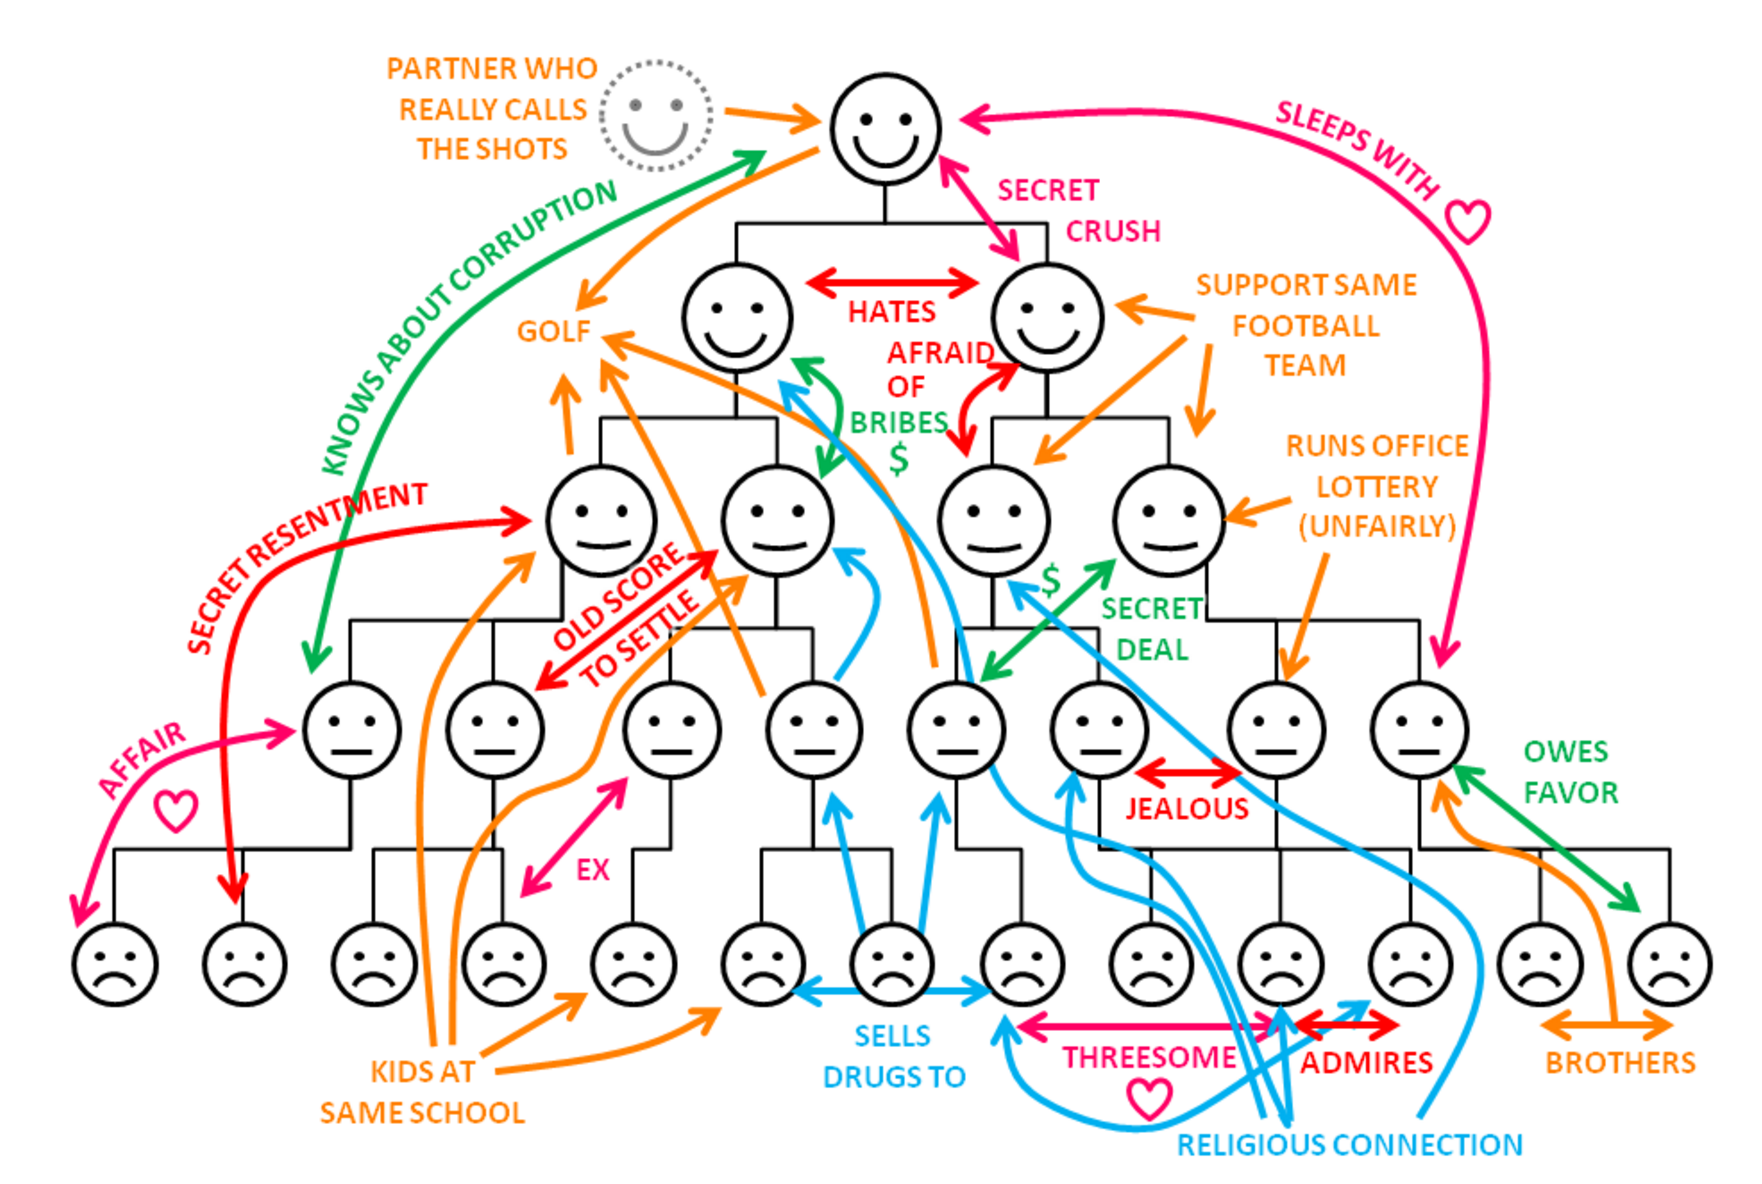
\includegraphics[scale=0.12]{top_down.png}
     \end{center}

\end{column}
\end{columns}

\end{frame}

%@@@@@@@@@@@@@@@@@@@@@@@@@@@@@@@@@@@@@@@@@@@@@@@@@
\begin{frame}
\frametitle{Synthesis}

\begin{itemize}
\item Efforts have been made to synthesize top down and bottom up into one approach;
\bigskip
\bigskip
\item Example: Advocacy Coalition Framework (Sabatier)
\begin{itemize}
\item Adopts bottom up approach;
\item Incorporates an abstract model with structural features of policy emphasized by the top-down theorists;
\item Intended to capture `policy subsystem';
\end{itemize}
\bigskip
\bigskip
\item Example: Message passing theories (e.g. Goggin et al.)
\begin{itemize}
\item \textbf{Clear messages} from \textbf{credible officials} received by \textbf{receptive implementers} w/ \textbf{sufficient resources} who implement policies \textbf{supported by affected groups} $=$ implementation success.
\item Strategic delay $=$ improved implementation of policies through innovation, policy learning, bargaining...
\end{itemize}
\end{itemize}

\end{frame}

%Implementation 794
%Top down approach 799
%Bottom up approach 809
%Synthesis of both 816
%Policy failure 822
%Learning from failures 827

%@@@@@@@@@@@@@@@@@@@@@@@@@@@@@@@@@@@@@@@@@@@@@@@@@
\begin{frame}
\frametitle{Birkland$+$ Model of Policy}
\begin{itemize}
\item Policy Domain: what substantive problems are under consideration?  This specifies:
\begin{itemize}
\item The actors involved, official actors who can make decisions $+$ stakeholders; 
\item Distribution of benefits/costs $\Rightarrow$ actor organization, e.g. iron triangle, policy community;
\item The systemic agenda; 
\end{itemize}
\bigskip
\item \color{black}Input-output Model;
\begin{itemize}
\item Actors: legislature, executive, bureaucrats, justices and the available levers;
\item Inputs: agenda setting (application of power/social construction, focusing events, indicator change driven esp by unofficial actors) sets goals, determines the causal model, which specifies the institutional agenda, and leads to the policies on the decision agenda;
\item Black box decision making (structured by median voter thm, Arrow's thm) works on the decision agenda;
\begin{itemize}
\item timing resembles incrementalism if driven by indicator change;
\item timing resembles punctuated equilibrium if driven by focusing events;
 \end{itemize}
\item Outputs (e.g. statute laws, rules, court decisions);
\end{itemize}
\bigskip
\item Outcomes: Feedback and iteration.
\end{itemize}
\end{frame}

%@@@@@@@@@@@@@@@@@@@@@@@@@@@@@@@@@@@@@@@@@@@@@@@@@
\begin{frame}
\frametitle{Birkland$+$ Model of Policy}
\begin{itemize}
\item Policy Domain: what substantive problems are under consideration?  This specifies:
\begin{itemize}
\item The actors involved, official actors who can make decisions $+$ stakeholders; 
\item Distribution of benefits/costs $\Rightarrow$ actor organization, e.g. iron triangle, policy community;
\item The systemic agenda; 
\end{itemize}
\bigskip
\item \color{black}Input-output Model;
\begin{itemize}
\item Actors: legislature, executive, bureaucrats, justices and the available levers;
\item Inputs: agenda setting (application of power/social construction, focusing events, indicator change driven esp by unofficial actors) sets goals, determines the causal model, which specifies the institutional agenda, and leads to the policies on the decision agenda;
\item Black box decision making, timing (incrementalism, punctuated eq) driven by indicators/focusing events, choice driven by e.g. median voter thm, Arrow's thm;
\begin{itemize}
\item \textbf{Round 1: works on decision agenda, leads to outputs (e.g. statute laws, rules, court decisions)};
\item \textbf{Round 2: Implementation, leads to outcomes};
 \end{itemize}
\end{itemize}
\bigskip
\item Outcomes: Feedback and iteration.
\end{itemize}
\end{frame}

%@@@@@@@@@@@@@@@@@@@@@@@@@@@@@@@@@@@@@@@@@@@@@@@@@
\begin{frame}
\frametitle{Policy failure}
\begin{columns}
\begin{column}{0.5\textwidth}

\begin{itemize}
\item Two issues:
\begin{itemize}
\item How do you establish that a policy failure has occurred?
\item How do you figure out why it has occurred?
\end{itemize}
\item Possible general explanations:
\begin{itemize}
\item Least worst;
\item Changing circumstances;
\item Policy interrelationship complexity;
\item Boundaries;
\item Excessive expectations;
\item Shot in the dark;
\item Inaccurate causal theory;
\item Use of ineffective tools;
\item Sound policy, failed implementation;
\item Political failure.
\end{itemize}
\end{itemize}
\end{column}
\begin{column}{0.5\textwidth}
    \begin{center}
     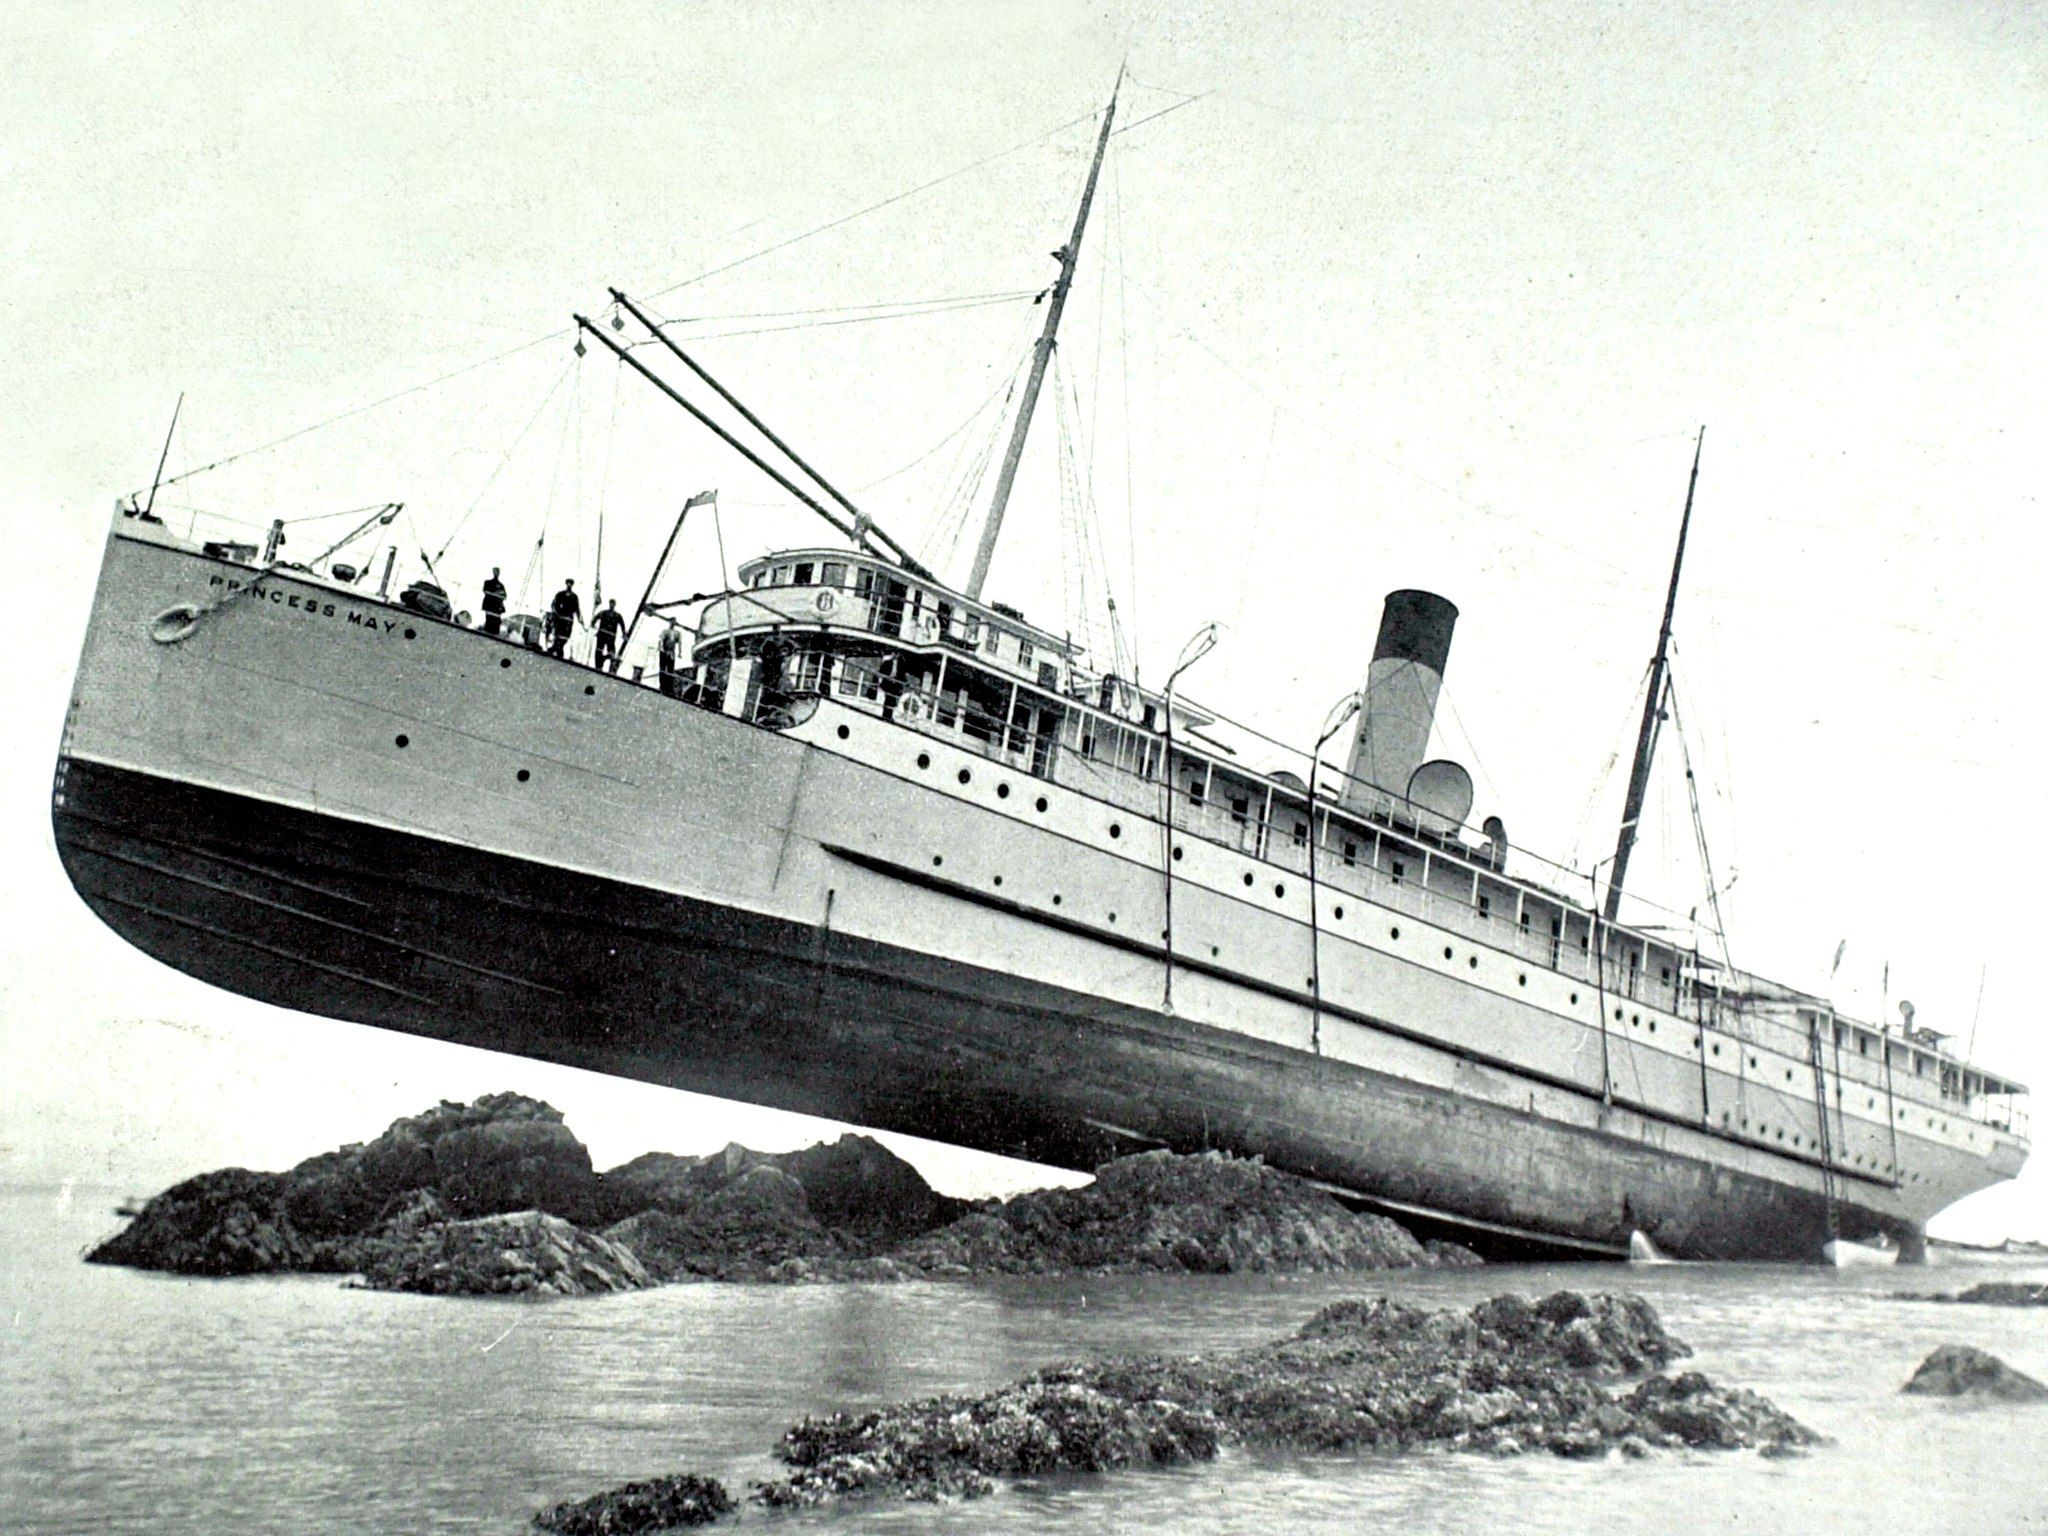
\includegraphics[scale=0.1]{ship_on_rocks.jpg}
     \end{center}

\end{column}
\end{columns}

\end{frame}

%@@@@@@@@@@@@@@@@@@@@@@@@@@@@@@@@@@@@@@@@@@@@@@@@@
\begin{frame}
\frametitle{Policy failure}

\begin{center}
\Huge \textbf{There are only intelligence failures and policy successes!}
\end{center}

\end{frame}

%@@@@@@@@@@@@@@@@@@@@@@@@@@@@@@@@@@@@@@@@@@@@@@@@@
\begin{frame}
\frametitle{Learning}

\begin{itemize}
\item Policy failure $=$ opportunity for learning (enduring changes to thought from experience)!
\bigskip
\item Individuals can learn -- can organizations learn?  In a passive sense:
\begin{itemize}
\item Information storage and retrieval;
\item Institutional memory;
\end{itemize}
\bigskip
\item In an active sense:
\begin{itemize}
\item Single loop learning: optimizing and adjusting policy;
\item Double loop learning: optimizing and adjusting fundamental values and logic that leads to policy;
\item Instrumental policy learning: effectiveness of policy tools;
\item Social policy learning: causes of problems;
\item Political learning: better arguments in policy debates.
\end{itemize}
\end{itemize}

\end{frame}

%@@@@@@@@@@@@@@@@@@@@@@@@@@@@@@@@@@@@@@@@@@@@@@@@@
\begin{frame}
\frametitle{Learning}

    \begin{center}
     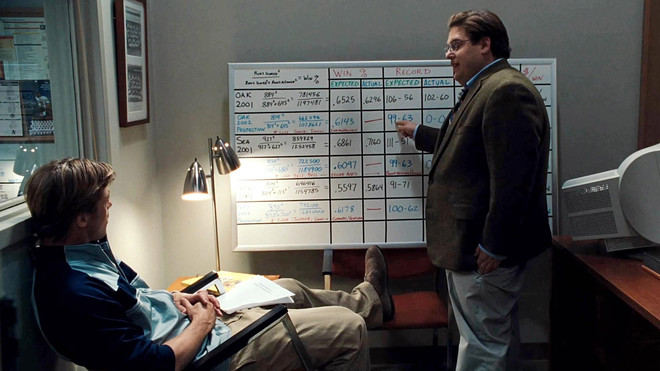
\includegraphics[scale=0.5]{moneyball.jpg}
     \end{center}

\end{frame}

%@@@@@@@@@@@@@@@@@@@@@@@@@@@@@@@@@@@@@@@@@@@@@@@@@
\begin{frame}
\frametitle{Birkland$+$ Model of Policy}
\begin{itemize}
\item Policy Domain: what substantive problems are under consideration?  This specifies:
\begin{itemize}
\item The actors involved, official actors who can make decisions $+$ stakeholders; 
\item Distribution of benefits/costs $\Rightarrow$ actor organization, e.g. iron triangle, policy community;
\item The systemic agenda; 
\end{itemize}
\bigskip
\item \color{black}Input-output Model;
\begin{itemize}
\item Actors: legislature, executive, bureaucrats, justices and the available levers;
\item Inputs: agenda setting (application of power/social construction, focusing events, indicator change driven esp by unofficial actors) sets goals, determines the causal model, which specifies the institutional agenda, and leads to the policies on the decision agenda;
\item Black box decision making, timing (incrementalism, punctuated eq) driven by indicators/focusing events, choice driven by e.g. median voter thm, Arrow's thm;
\begin{itemize}
\item Round 1: works on decision agenda, leads to outputs (e.g. statute laws, rules, court decisions);
\item Round 2: Implementation, leads to outcomes;
 \end{itemize}
\end{itemize}
\bigskip
\item Outcomes: Feedback and iteration.
\end{itemize}
\end{frame}

%@@@@@@@@@@@@@@@@@@@@@@@@@@@@@@@@@@@@@@@@@@@@@@@@@
\begin{frame}
\frametitle{Birkland$+$ Model of Policy}
\begin{itemize}
\item Policy Domain: what substantive problems are under consideration?  This specifies:
\begin{itemize}
\item The actors involved, official actors who can make decisions $+$ stakeholders; 
\item Distribution of benefits/costs $\Rightarrow$ actor organization, e.g. iron triangle, policy community;
\item The systemic agenda; 
\end{itemize}
\bigskip
\item \color{black}Input-output Model;
\begin{itemize}
\item Actors: legislature, executive, bureaucrats, justices and the available levers;
\item Inputs: agenda setting (application of power/social construction, focusing events, indicator change driven esp by unofficial actors) sets goals, determines the causal model, which specifies the institutional agenda, and leads to the policies on the decision agenda;
\item Black box decision making, timing (incrementalism, punctuated eq) driven by indicators/focusing events, choice driven by e.g. median voter thm, Arrow's thm;
\begin{itemize}
\item Round 1: works on decision agenda, leads to outputs (e.g. statute laws, rules, court decisions);
\item Round 2: Implementation, leads to outcomes;
 \end{itemize}
\end{itemize}
\bigskip
\item Outcomes: \textbf{Feedback from failure and success, learning leads to iteration and updates}.
\end{itemize}
\end{frame}

%@@@@@@@@@@@@@@@@@@@@@@@@@@@@@@@@@@@@@@@@@@@@@@@@@
\begin{frame}
\frametitle{Time for Science!}

\begin{itemize}
\item Lasswell: we need scientific (quantitative, falsification-based (Popper)) study of policy to better control the world;
\bigskip
\bigskip
\item Falsification:
\begin{itemize}
\item Theory $\Longrightarrow$ Testable Hypothesis;
\item Predicate logic tells us that: Testable Hypothesis inconsistent w/ data $\Longrightarrow$ Theory is wrong;
\item Logical fallacy: Testable Hypothesis consistent w/ data $\Longrightarrow$ Theory is true;
\end{itemize}
\bigskip
\bigskip
\item Things to keep in mind:
\begin{itemize}
\item All models are wrong but some models are useful;
\item Science $\neq$ statistics, but statistics is a VERY robust way to check for falsification;
\item Science NEVER proves theory to be `true'.
\end{itemize}
\end{itemize}

\end{frame}

%%@@@@@@@@@@@@@@@@@@@@@@@@@@@@@@@@@@@@@@@@@@@@@@@@@
%\begin{frame}
%\frametitle{Models of the Policy Process: Stages}
%    \begin{center}
%     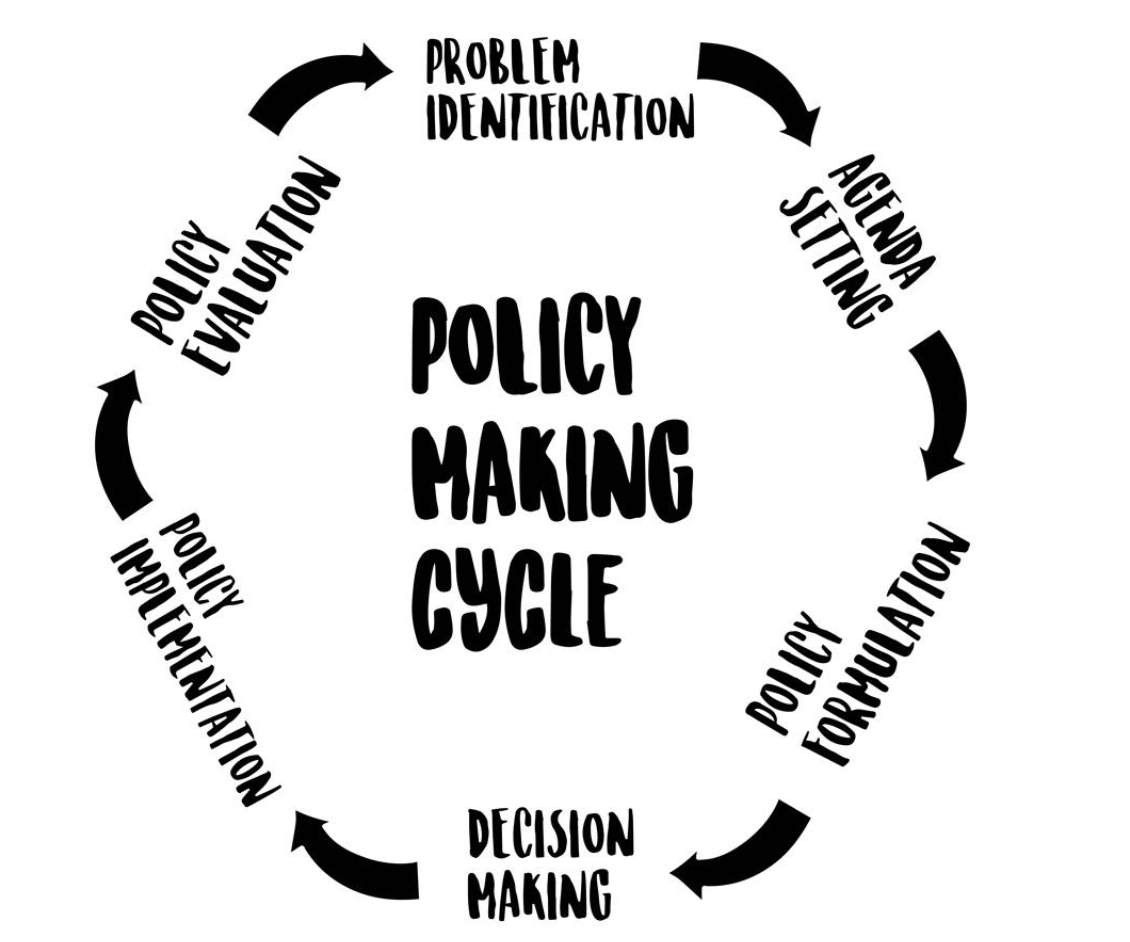
\includegraphics[scale=0.4]{policy_process.png}
%     \end{center}
%\end{frame}

%@@@@@@@@@@@@@@@@@@@@@@@@@@@@@@@@@@@@@@@@@@@@@@@@@
\begin{frame}
\frametitle{Models of the Policy Process: Streams (Kingdon)}
\begin{columns}
\begin{column}{0.5\textwidth}

\begin{itemize}
\item \textbf{Political stream} -- e.g. electoral change, state of public opinion;
\bigskip
\item \textbf{Problem stream} -- e.g. problem definition, attributes, whether it is getting better or worse, more or less attention;
\bigskip
\item \textbf{Policy stream} -- e.g. articulation of better policies, potential ideas that could be solutions;
\end{itemize}
\end{column}
\begin{column}{0.5\textwidth}

    \begin{center}
     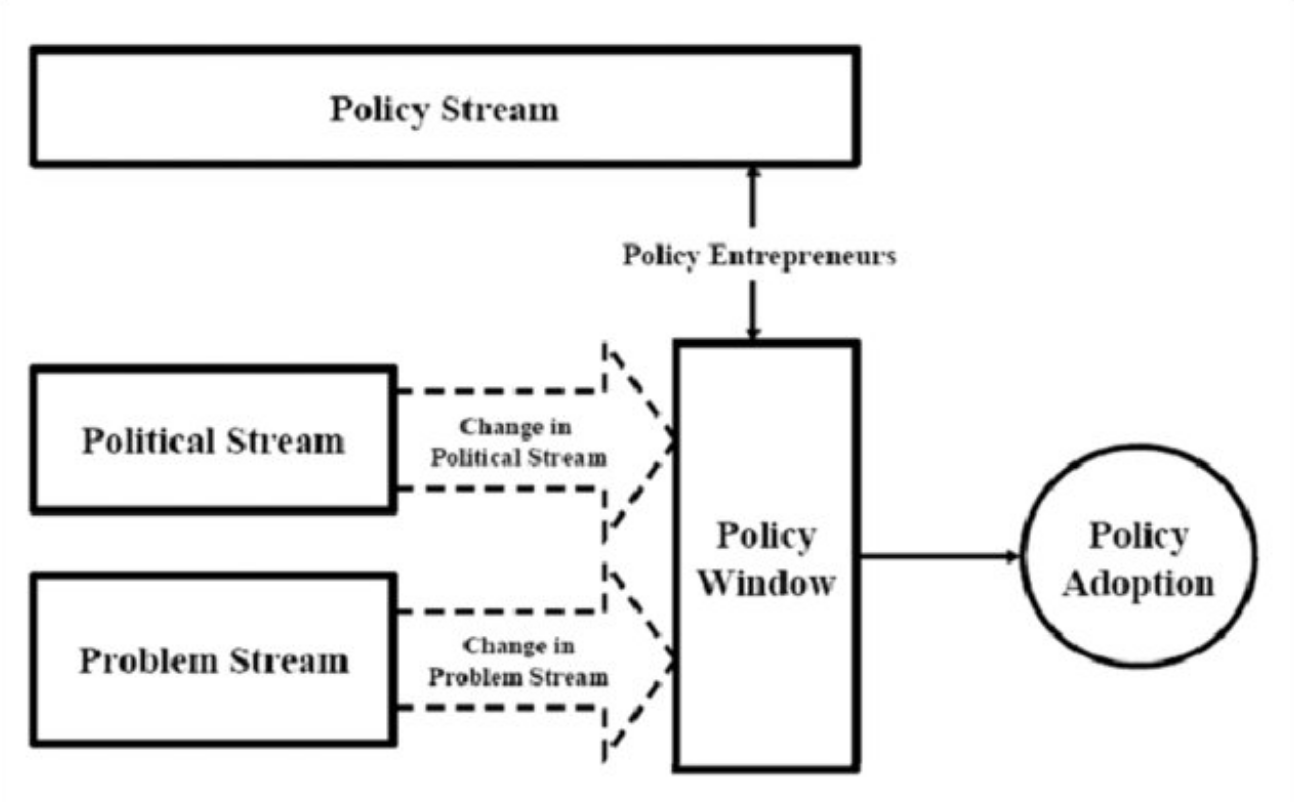
\includegraphics[scale=0.3]{windows.png}
     \end{center}
\end{column}
\end{columns}

\end{frame}

%@@@@@@@@@@@@@@@@@@@@@@@@@@@@@@@@@@@@@@@@@@@@@@@@@
\begin{frame}
\frametitle{Models of the Policy Process: Streams (Kingdon)}
\begin{columns}
\begin{column}{0.5\textwidth}

\begin{itemize}
\item `Crossing' or `meeting' of the streams creates a `policy window' where change can happen;
\bigskip
\item This is a \textbf{necessary but NOT sufficient condition}...
\bigskip
\item Criticism: incomplete -- can't actually offer predictions about policy change.
\end{itemize}
\end{column}
\begin{column}{0.5\textwidth}

    \begin{center}
     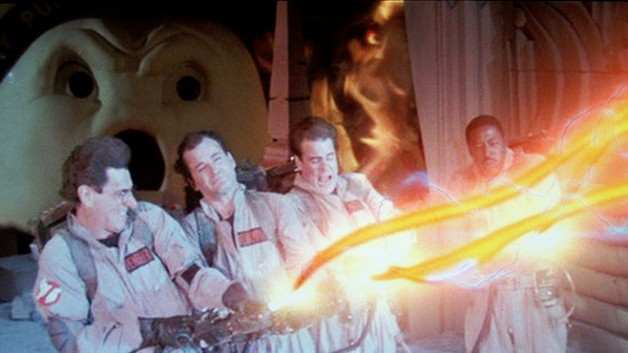
\includegraphics[scale=0.3]{streams2.jpeg}
     \end{center}
\end{column}
\end{columns}

\end{frame}

%@@@@@@@@@@@@@@@@@@@@@@@@@@@@@@@@@@@@@@@@@@@@@@@@@
\begin{frame}
\frametitle{Models of the Policy Process: Punctuated Equilibrium (Baumgartner and Jones)}

\begin{itemize}
\item Central ideas:
\begin{itemize}
\item Policy monopoly: closed system of most important actors (e.g. smoke filled room);
\item Stable parameter: balance of power among interest groups;
\item Dynamic parameters: public understanding of problems, rarely balance of power;
\end{itemize}
\bigskip
\item Policy monopoly breakdown = media attention, venue shopping;
\bigskip
\item \textbf{Model Prediction}: long periods of policy \textbf{stability broken} by short periods of \textbf{sudden change}.
\end{itemize}

\end{frame}

%@@@@@@@@@@@@@@@@@@@@@@@@@@@@@@@@@@@@@@@@@@@@@@@@@
\begin{frame}
\frametitle{Models of the Policy Process: Institutional Analysis and Development (Ostrom)}

\begin{itemize}
\item Used to understand \textbf{common pool} policy problems, e.g. public water resources;
\bigskip
\item Built on rational choice -- utility-maximizing actors `satisfice' -- optimize given constraints -- expressed as \textbf{rules} within \textbf{institutions};
\bigskip
\item Two important parts:
\begin{itemize}
\item Action arena -- community attributes, rules-in-use, the problem at hand, and the actors;
\item Actors characterized by four variables:
\begin{itemize}
\item Resources;
\item Preferences for different states of the world;
\item Information processing;
\item Optimization criteria: efficiency, equity, accountability, rule-following, adaptability.
\end{itemize}
\end{itemize}
\bigskip
\item \textbf{Model Prediction}: people can, under `proper conditions,' \textbf{form institutions for common pool resource management}.
\end{itemize}
\end{frame}

%@@@@@@@@@@@@@@@@@@@@@@@@@@@@@@@@@@@@@@@@@@@@@@@@@
\begin{frame}
%\frametitle{Models of the Policy Process: Advocacy Coalition Framework (Sabatier)}

\begin{center}
\huge\textbf{Advocacy Coalition Framework Deep Dive}
\end{center}

\end{frame}

%@@@@@@@@@@@@@@@@@@@@@@@@@@@@@@@@@@@@@@@@@@@@@@@@@
\begin{frame}
\frametitle{Models of the Policy Process: Advocacy Coalition Framework (Sabatier)}

\begin{itemize}
\item Premise 1: falsification on time scale of decade $+$;
\bigskip
\bigskip
\item Premise 2: focus on policy subsystems -- interaction of actors from different institutions interested in a policy area;
\bigskip
\bigskip
\item Premise 3: public policies $=$ belief systems $=$ sets of value priorities and causal assumptions about how to achieve them.
\end{itemize}

\end{frame}

%@@@@@@@@@@@@@@@@@@@@@@@@@@@@@@@@@@@@@@@@@@@@@@@@@
\begin{frame}
\frametitle{Models of the Policy Process: Advocacy Coalition Framework (Sabatier)}
\begin{itemize}
\item Internal/External stable parameters:
\bigskip
\begin{itemize}
\item Basic attributes of the problem (e.g. characteristics of goods, quantifiability);
\bigskip
\item Distribution of natural resources (e.g. overall wealth);
\bigskip
\item Fundamental cultural values/social structure (e.g. norms, group level power);
\bigskip
\item Basic legal structure (e.g. constitution, filibuster);
\end{itemize}
\bigskip
\item Because these are inherently slow to change they aren't usually objects for strategy;
\bigskip
\item Explains across, not within.
\end{itemize}

\end{frame}

%@@@@@@@@@@@@@@@@@@@@@@@@@@@@@@@@@@@@@@@@@@@@@@@@@
\begin{frame}
\frametitle{Models of the Policy Process: Advocacy Coalition Framework (Sabatier)}

\begin{itemize}
\item Dynamic parameters:
\bigskip
\begin{itemize}
\item Changes in socio-economic conditions and technology (e.g. public opinion, electric vehicles);
\bigskip
\item Systemic governing coalitions (e.g. an election);
\bigskip
\item Policy decisions in other policy subsystems (e.g. energy independence/pollution control);
\end{itemize}
\bigskip
\item Can change very quickly and so are candidates for strategic manipulation;
\bigskip
\item Explains across and within.
\end{itemize}

\end{frame}

%@@@@@@@@@@@@@@@@@@@@@@@@@@@@@@@@@@@@@@@@@@@@@@@@@
\begin{frame}
\frametitle{Models of the Policy Process: Advocacy Coalition Framework (Sabatier)}

\begin{itemize}
\item What is a policy subsystem?
\bigskip
\item Boundaries: the set of actors currently involved in dealing with a policy problem $+$ those who \textbf{could} become involved;
\bigskip
\item Origins: dissatisfaction with problem neglect $=$ breakaway to form new subsystem;
\bigskip
\item Actors: diverse set... e.g.:
\begin{itemize}
\item The EPA;
\item Relevant Congressional committees;
\item Peer agencies involved in pollution control (e.g. DOE);
\item Pollution emitters and their trade associations, unions, etc.;
\item Manufacturers of pollution control equipment;
\item Environmental and public health groups;
\item State and local pollution control agencies
\item Research institutions and consulting firms;
\item Journalists who regularly write on the issue.
\end{itemize}
\end{itemize}

\end{frame}

%@@@@@@@@@@@@@@@@@@@@@@@@@@@@@@@@@@@@@@@@@@@@@@@@@
\begin{frame}
\frametitle{Models of the Policy Process: Advocacy Coalition Framework (Sabatier)}

\begin{itemize}
\item How are actors organized?  Two groups...
\bigskip
\item Advocacy coalitions --  \textbf{people} (why not institutions?) from a variety of positions that:
\begin{itemize} 
\item share a belief system (deep/near/secondary basic values, causal assumptions, perceptions of the problem) and 
\item who coordinate activity to translate beliefs into policies;
\item are endowed with resources (e.g. power) that can be used for this;
\item Example: `Clean air' coalition vs `Economic feasibility' coalition;
\end{itemize}
\bigskip
\item Policy brokers: individuals primarily concerned with keeping level of political conflict within acceptable bounds;
\end{itemize}

\end{frame}

%@@@@@@@@@@@@@@@@@@@@@@@@@@@@@@@@@@@@@@@@@@@@@@@@@
\begin{frame}
\frametitle{Models of the Policy Process: Advocacy Coalition Framework (Sabatier)}

\begin{itemize}
\item How does this all come together to offer predictions about policy making?
\bigskip
\bigskip
\item Actors are expected utility maximizers with well defined preferences and bounded rationality;
\bigskip
\bigskip
\item Two processes interact to govern policy change:
\begin{itemize}
\item Structure of belief systems $\Rightarrow$ changes in beliefs $\Rightarrow$ attempted changes in policy;
\item Shifts in dynamic parameters;
\end{itemize}


\end{itemize}

\end{frame}

%@@@@@@@@@@@@@@@@@@@@@@@@@@@@@@@@@@@@@@@@@@@@@@@@@
\begin{frame}
\frametitle{Models of the Policy Process: Advocacy Coalition Framework (Sabatier)}

    \begin{center}
     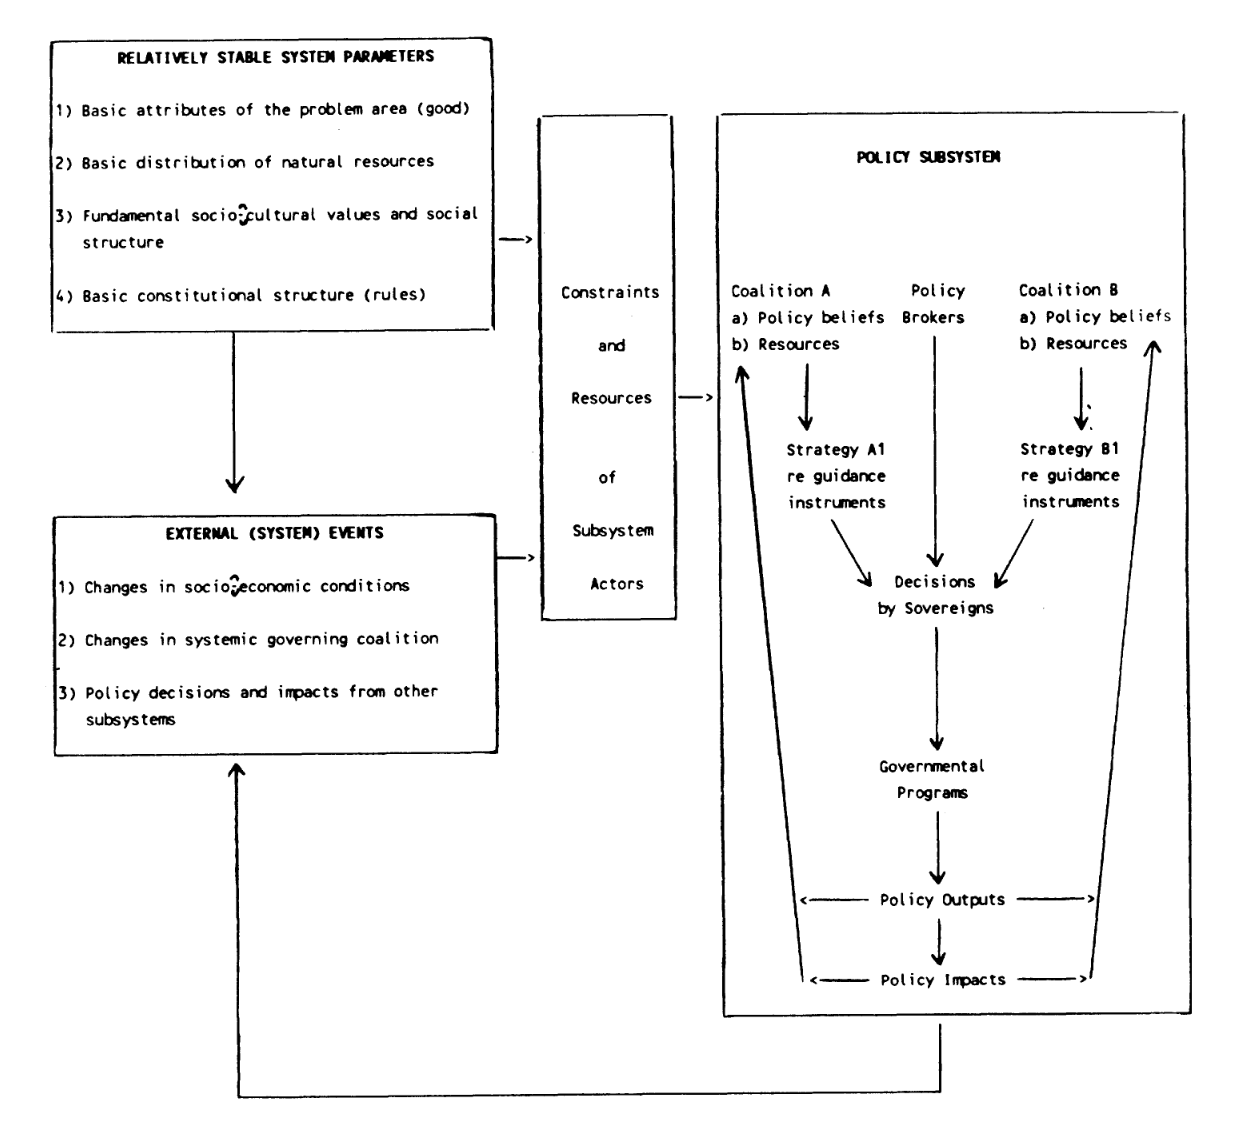
\includegraphics[scale=0.35]{ACF.png}
     \end{center}

\end{frame}

%@@@@@@@@@@@@@@@@@@@@@@@@@@@@@@@@@@@@@@@@@@@@@@@@@
\begin{frame}
\frametitle{Models of the Policy Process: Advocacy Coalition Framework (Sabatier)}

\begin{itemize}
\item \textbf{Model Predictions:}
\begin{itemize}
\item On major controversies lineup of allies/opponents is stable;
\item Intra-coalition consensus on core but not secondary issues;
\item Change secondary before core;
\item Core of govt prog unlikely to change so long as instituting advocacy coalition is in power;
\item Core of govt prog unlikely to change w/o shocks via dynamic parameters;
\item Intermediate conflict $\Rightarrow$ policy learning/belief change;
\item Fora w/ strong professional norms and participation reqs $\Rightarrow$ policy learning/belief change;
\item Accepted quantification $\Rightarrow$ policy learning/belief change;
\item Natural systems $\Rightarrow$ policy learning/belief change;
\end{itemize}
\end{itemize}

\end{frame}

%@@@@@@@@@@@@@@@@@@@@@@@@@@@@@@@@@@@@@@@@@@@@@@@@@
\end{document}








